%!TEX TS-program = ./make.zsh

\documentclass[a4paper,12pt]{article}

\title{The Effect of Hole Ice on the Propagation and Detection of Light in IceCube}
\author{Sebastian Fiedlschuster}
\newcommand\shorttitle{Hole Ice}
\newcommand\entwurf{\today}

% TODO: Customze layout here.

\usepackage{microtype}
\usepackage{parskip}

\usepackage[T1]{fontenc}
\usepackage[utf8]{inputenc}
\usepackage{lipsum}
\usepackage{graphicx}
\usepackage[font=footnotesize]{caption}

\newcommand\image[1]{\includegraphics[width=\textwidth]{img/#1}}
\newcommand\smallerimage[1]{\centering\includegraphics[width=0.6\textwidth]{img/#1}}
\newcommand\halfimage[1]{\includegraphics[width=0.48\textwidth]{img/#1}}
\newcommand\halfcropimage[2]{\includegraphics[width=0.48\textwidth, trim={#2}, clip]{img/#1}}
\newcommand\thirdimage[1]{\includegraphics[width=0.32\textwidth]{img/#1}}

\newcommand\fig[2]{
  \begin{figure}[htb]
    \begin{margincap}
      \centering
      \image{#1}
      \caption{#2}
    \end{margincap}
  \end{figure}
}

\usepackage{placeins} % implements \FloatBarrier

\usepackage{fontawesome}

\usepackage[font=scriptsize, position=b]{subcaption}

% http://pgfplots.sourceforge.net/pgfplots.pdf
\usepackage{pgfplots}
% Pandoc (http://pandoc.org) is used in the `Makefile' to pre-process
% `text/*.md.tex` files from markdown to latex. This way, one may use
% lists, section headings etc. in the .md.tex files.

% Pandoc requires a `\tightlist`.
% https://tex.stackexchange.com/a/258486/70789
\providecommand{\tightlist}{%
  \setlength{\itemsep}{0pt}\setlength{\parskip}{0pt}}
% Markierungen mit `\todo{foo}`, `\mref{schiller}`, `\frage{foo}` einfügen.

\usepackage{color}

% Markierung einfügen (Kommentar während der Bearbeitung) % Parameter: Art, Kommentar
\newcommand{\markierung}[2]{
        \textcolor{red}{\textbf{#1:} #2} \\
}

\newcommand{\todo}[1]{\markierung{To do}{#1}} % ToDo-Kommentar einfügen, Parameter: Kommentar
\newcommand{\mref}[1]{\markierung{Verweis einfügen}{#1}} % Fehlenden Verweis markieren, Parameter: Kommentar
\newcommand\frage[1]{\markierung{Frage}{#1}} % Frage

\usepackage[backend=biber]{biblatex}

\usepackage{amsmath}
\usepackage{amssymb}

% Vectors
\renewcommand{\vec}[1]{\overrightarrow{#1}}
\newcommand{\norm}[1]{\left\lVert#1\right\rVert}
\newcommand{\len}[1]{\overline{#1}}

% Comparison operators
\newcommand{\identical}{\equiv}

% Sets
\newcommand{\reals}{\mathbb{R}}
\newcommand{\naturals}{\mathbb{N}}

% Constants
\newcommand{\e}{\mathrm{e}}
% Highlighted code listings, https://ctan.org/pkg/minted
%
% This requires pygments.
%
%     pip install Pygments
%     cd /Library/TeX/texbin
%     sudo ln -s `which pygmentize` pygmentize
%     sudo tlmgr install fvextra
%     sudo tlmgr update minted
%
\usepackage[outputdir=./build]{minted}

\setminted{
  tabsize=2, linenos, breaklines, autogobble, breakautoindent, frame=lines, framesep=2mm
}

\newenvironment{python}{\minted{python}}{\endminted}
\newcommand\pythoninput[1]{\inputminted{python}{#1}}

\newenvironment{ccode}{\minted{c}}{\endminted}
\newcommand\appendixref[1]{appendix \ref{#1}, p.\,\pageref{#1}}
\usepackage[ngerman, english]{babel}

\usepackage{iflang}

\IfLanguageName{ngerman}{
  \newcommand\pageStr{Seite}
}{
  \newcommand\pageStr{Page}
}
\usepackage[explicit]{titlesec}

% The current section, subsection and subsubsection
% are stored in these commands, such that they can
% be included in the page header.
%
\newcommand\currentsection{}
\newcommand\currentsubsection{}
\newcommand\currentsubsubsection{}

% \preparesectionmarks needs to be called after \pagestyle in order to
% copy the current section titles into the header.
% https://de.wikibooks.org/wiki/LaTeX-Wörterbuch:_chaptermark
%
\newcommand\preparesectionmarks{
  \renewcommand\sectionmark[1]{\renewcommand\currentsection{##1}}
  \renewcommand\subsectionmark[1]{\renewcommand\currentsubsection{##1}}
  \renewcommand\subsubsectionmark[1]{\renewcommand\currentsubsubsection{##1}}
}

% http://tug.ctan.org/macros/latex/contrib/titlesec/titlesec.pdf
% https://tex.stackexchange.com/a/59727/70789
%
% \titleformat{⟨command⟩}[⟨shape⟩]{⟨format⟩}{⟨label⟩}{⟨sep⟩}{⟨before-code⟩}[⟨after-code⟩]
%\titleformat{\section}{\Large\bfseries}{\thesection\quad}{0cm}{\renewcommand{\currentsection}{#1} #1}
%\titleformat{\subsection}{\large\bfseries}{\thesubsection\quad}{0cm}{\renewcommand{\currentsubsection}{#1}#1}
%\titleformat{\subsubsection}{\normalsize\bfseries}{\thesubsubsection\quad}{0cm}{\renewcommand{\currentsubsubsection}{#1}#1\emph{}}

% Start sections on odd pages:
% https://tex.stackexchange.com/a/51926/70789
%
\let\oldsection\section
\def\section{\cleardoublepage\oldsection}
% This file is responsible for the page header.

\usepackage{fancyhdr}

\pagestyle{fancy}
\fancyhf{}

% This provides \currentsection, \currentsubsection and \currentsubsubsection.
% See: lib/section.tex
%
\preparesectionmarks

\fancyhead[L,EL]{%
  \footnotesize
  \minipage{10cm}%
    \textsf{%
      \textbf{{\dokumententitel}},
			\dokumentid,
			\ifthenelse{\equal{\entwurf}{}}{
				\datum
			}{
				\textcolor{red}\entwurf\normalcolor
			} \\
			\ifthenelse{\equal{\currentsubsection}{}}{}{\thesubsection \ \ }\currentsection\ifthenelse{\equal{\currentsubsection}{}}{}{: \currentsubsection}
		}
  \endminipage
}

\fancyhead[C]{}

\fancyhead[OR]{\logo}

\renewcommand{\headrulewidth}{0.0pt} %obere Trennlinie
\addtolength{\headheight}{2\baselineskip} % noch etwas Platz

\fancyfoot[OL]{}
\fancyfoot[C]{}
\fancyfoot[OR,EL]{\vspace{2cm}\fancyfootfont{ Seite \thepage}}

\renewcommand{\footrulewidth}{0.0pt} %untere Trennlinie
\usepackage{xspace}

\newcommand\unit[1]{\text{\,#1}\xspace}
\newcommand\m{\unit{m}}
\newcommand\cm{\unit{cm}}
\newcommand\mm{\unit{mm}}

\newcommand\ns{\unit{ns}}

\usepackage{siunitx}
\usepackage{physics}
\usepackage{hepnames}
\usepackage{tabularx}
\usepackage{multirow}

% Tabellenanpassung
\newcommand{\oldarraystretch}{}
\newcolumntype{C}{>{\centering\arraybackslash}X}
\newcolumntype{R}{>{\raggedleft\arraybackslash}X}
\newcolumntype{L}{>{\raggedright\arraybackslash}X}
%\renewcommand\tabularxcolumn[1]{m{#1}}
\newenvironment{tabelle}[1]%
{%
\renewcommand{\oldarraystretch}{\arraystretch}
  \renewcommand{\arraystretch}{1.5} % Tabellenabstände vergrößern
  \noindent\tabularx{\textwidth}{#1}
}{%
  \endtabularx
  \renewcommand{\arraystretch}{\oldarraystretch}
}

% Hyperlinks und Kreuzverweise zu anderen Dokumenten
\usepackage[hyphens]{url}
%\usepackage{xr}
%\usepackage{xr-hyper}
\usepackage[breaklinks]{hyperref}
\usepackage[hyphenbreaks]{breakurl}

% https://tex.stackexchange.com/a/50754/70789
% % \hypersetup{
% %   colorlinks = false,
% %   linkbordercolor = {white},
% % }

% https://tex.stackexchange.com/a/668/70789
\urlstyle{sf}

\usepackage{csquotes} % Enables \enquote{text in quotation marks}

\newcommand\noun[1]{\textsc{#1}}


% Differentials
\renewcommand\d{\text{d}}
\newcommand\dx{\d x}
\newcommand\dn{\d n}

% Quantities
\newcommand\abs{_\text{abs}}
\newcommand\sca{_\text{sca}}
\newcommand\esca{_\text{e}}
\newcommand\hi{^\text{H}}
\newcommand\lambdaabs{\lambda\abs}
\newcommand\dom{_\text{DOM}}
\newcommand\domhi{_\text{DOM,HI}}
\newcommand\domdima{_\text{DOM,HI}^\text{Dima}}

% Reference to issues on the cd rom and on the web
\newcommand\issue[1]{\texttt{issues/#1} on the cdrom as well as online at \url{https://github.com/fiedl/hole-ice-study/issues/#1}}
\newcommand\script[1]{\texttt{hole-ice-study/scripts/#1} on the cdrom as well as online at \url{https://github.com/fiedl/hole-ice-study/tree/master/scripts/#1}}

% Follow-up marker, not sure how to use this, yet.
\newcommand\followup{}

% Special names
\newcommand\authorname[1]{\noun{#1}\xspace}
\newcommand\softwarename[1]{\noun{#1}\xspace}
\newcommand\clsim{\softwarename{clsim}}
\newcommand\ppc{\softwarename{ppc}}
\newcommand\photonics{\softwarename{Photonics}}
\newcommand\steamshovel{\softwarename{Steamshovel}}
\newcommand\rongen{\authorname{Rongen}}
\newcommand\chirkin{\authorname{Chirkin}}

% Hole-ice parameters
\newcommand\HH{\mathcal{H}}

%\includeonly{}

\bibliography{diplomarbeit}
\begin{document}
  \maketitle

  \newpage
  \setcounter{tocdepth}{2}
  \tableofcontents

  \section{Introduction}
\label{sec:intro}

\icecube is a neutrino observatory located at Earth's South Pole. It
uses a cubic-kilometer of glacial ice as detector medium where secondary
particles from neutrino interactions produce light as they move through
the ice. The light is detected by an array of photo detector modules
that are deployed throughout the ice. \cite{evidence2013}

The primary scientific objective of \icecube is the study of neutrinos
with energies ranging from \(10\TeV\) to \(10\PeV\) produced in
astrophysical processes, and the identification and characterization of
their sources. In collaboration with other neutrino detectors as
\noun{Antares}, with optical, x-ray, gamma-ray, radio, and
gravitational-wave observatories, \icecube participates in efforts for
multi-messenger astronomy. Other objectives include the indirect
detection of dark matter, the search for other exotic particles, and the
study of neutrino-oscillation physics.
\cite{instrumentation, evidence2013}

As \icecube detects neutrinos indirectly through the interaction with
other particles, involving a chain of processes and components, a key
requirement for precise measurements is to minimize uncertainties for
each process and component involved. Some components such as technical
instruments in the detector modules can be tested and calibrated in
isolation in laboratories. Other components involved such as the glacial
ice cannot be extracted and need to be studied where they are.
Uncertainties concerning the properties of the glacial ice can affect
the precision for measurements of the direction of the detected
neutrinos by several percent. \cite{wrede}

All light that is detected by the detector modules needs to travel
through the refrozen water of the drill holes that were needed to deploy
the detector modules within the ice. This so-called \textit{hole ice}
may have properties significantly different from the surrounding bulk
ice regarding the propagation of light through this medium. The
properties of the hole ice are less known than the properties of the
bulk ice and pose the largest systematic uncertainty for study of
neutrino oscillations and a number of other analyses. \cite{icrc17pocam}

This study aims to provide the necessary tools to improve detector
calibration by introducing the means to simulate the propagation of
light through the hole ice. By comparing different simulation scenarios,
involving hole ice of different respective properties, to calibration
data, it is then possible to study the properties of the hole ice and
its effect on the propagation of light, and on the detection of light by
the detector modules, reducing the systematic uncertainties imposed by
the hole ice, and in the long run improving the precision of the
\icecube observatory.

After providing some background information in sections
\ref{sec:theoretical_background} to \ref{sec:simulation_background}, two
algorithms and their integration into the existing \icecube software
framework will be presented in section \ref{sec:methods} that allow to
simulate the direct propagation of photons through hole ice of different
properties. The validity of the algorithms will be supported by a series
of tests and cross checks in section
\ref{sec:unit_tests_and_cross_checks}.

Examples of application such as the simulation of one or several
hole-ice cylinders with different sizes and photon scattering lengths,
the simulation of shadowing cables, and a calibration method using LED
flasher data are given in section\nbsp\ref{sec:applications}.
Section\nbsp\ref{sec:discussion} presents a brief comparison of methods
and preliminary results to other studies. This section also discusses
performance considerations and lists ice properties not considered in
this study.

The material needed to reproduce this study is provided on the
accompanying CD-ROM and can be found online at
\url{https://github.com/fiedl/hole-ice-study}.

  \section{Theoretical Concepts}
\label{sec:theoretical_background}

\subsection{Neutrinos}
\label{sec:neutrinos}

Neutrinos are particles that primarily interact with other particles
through the \textit{weak interaction} and have very small probabilities
of interacting with other particles, allowing them to cross matter
almost unhindered. While this makes them interesting messenger particles
for observing far-distant astronomical sources and phenomena, because
they are long ranging and arrive undeflected and unscattered, it also
makes their detection challenging due to the large amount of detector
medium required. \cite{lexikonderphysik, instrumentation}

Within the \textit{standard model of particle physics} (see figure
\ref{fig:Pheith9i}), the electron neutrino, \(\Pnue\), the muon
neutrino, \(\Pnum\), and the tau neutrino \(\Pnut\), are
\textit{leptons} without electrical charge and couple to the \(\PWpm\)
and \(\PZz\) bosons.

\begin{figure}[htbp]
  \smallerimage{standard-model}
  \caption{Particles of the standard model of particle physics. Together with the electron, the muon, and the tau, the neutrinos form the group of leptons, which do not participate in \textit{strong interactions}. As neutrinos also do not participate in the \textit{electromagnetic interaction}, their primary interaction channel is through \textit{weak interactions}. Image based on: \cite{standardmodel}}
  \label{fig:Pheith9i}
\end{figure}

As the \textit{mass eigenstates} \(\Pnu_i\) of neutrinos that describe
neutrinos in the context of their propagation through spacetime, are not
identical to the neutrino \textit{flavor eigenstates} \(\Pnulepton\)
that describe neutrinos participating in weak interactions, neutrinos
are subject to quantum mechanical phenomena as
\textit{neutrino oscillations}. \cite{particledatareview}

\[
  \ket{\Pnulepton} = \sum_{i=1}^N U_{\Plepton i}\,\ket{\Pnu_i}, \ \ \ \Plepton \in \{ \Pe, \Pmu, \Ptau \}
\]

Determining the mixing matrix \(U_{\Plepton i}\) that connects the mass
eigenstates to the flavor eigenstates, is part of \icecube's scientific
objectives.

Neutrinos generated by interactions of cosmic-ray particles in the
Earth's atmosphere, \textit{atmospherical neutrinos}, have energies in
the GeV to TeV scale. \textit{Astrophysical neutrinos}, generated by
high-energy phenomena in the universe, have energies up to the PeV
scale. \cite{instrumentation}

\subsection{Neutrino Interactions Relevant to \icecube}
\label{sec:neutrino_interactions}

The primary interaction channel for detecting neutrinos in \icecube is
deep-inelastic scattering of neutrinos with quarks of nuclei in the
detector material or nearby rock (see figure \ref{fig:Phei1oob}).
\cite{energyreco}

\begin{figure}[htbp]
  \centering
  \subcaptionbox{Neutral-current neutrino interaction through $\PZz$ bosons.}{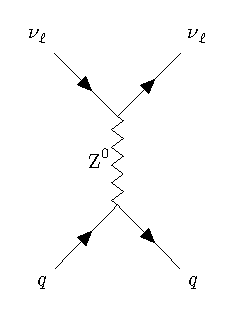
\includegraphics[width=0.3\textwidth]{img/feynman-neutral}\vspace*{2mm}}\hspace{1cm}
  \subcaptionbox{Charged-current neutrino interactions through $\PWpm$ bosons.}{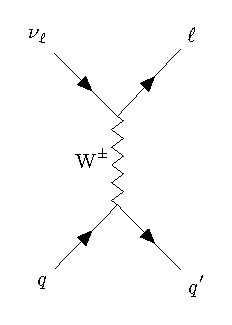
\includegraphics[width=0.3\textwidth]{img/feynman-charged}}
  \caption{Feynman diagrams showing neutrinos $\Pnulepton$ interacting with quarks~$\Pquark$ of nuclei of the ice or nearby rock through $\PZz$ and $\PWpm$ bosons, producing leptons~$\Plepton$ (electrons~$\Pe$, muons~$\Pmu$, tau particles~$\Ptau$) and quarks. Time evolves to the right in these diagrams.}
  \label{fig:Phei1oob}
\end{figure}

These interactions lead to three different kind of event signatures in
the \icecube detector, visualized in figure \ref{fig:eeQuaef6}.

\paragraph{Shower- or Cascade-Like Events}

In both, interactions through \(\PZz\) bosons
(\textit{neutral-current interactions}) and through \(\PWpm\) bosons
(\textit{charged-current interactions}), hadronic showers are created as
energy is transferred from the incoming neutrino to the outgoing quark.
Hadronic showers are particle cascades originating from hadron
particles. If the outgoing lepton is an electron, this may also create
an accompanying electromagnetic shower, which is a particle cascade
originating from particles primarily interacting through the
electromagnetic interaction. \cite{energyreco}

\begin{align*}
  & \text{neutral current:} & \Pnulepton + \text{nucleon} & \rightarrow \Pnulepton + \text{hadron} \ \ \ \ \ \ \Plepton \in \{ \Pe, \Pmu, \Ptau \}                             & \\
  &                         &                             & \rightarrow \Pnulepton \text{ (escapes) } + \text{hadronic shower}  & \\ \\
  & \text{charged current:} & \Pnue + \text{nucleon}      & \rightarrow \Pe + \text{hadron}                                     & \\
  &                         &                             & \rightarrow \text{electromagnetic shower} + \text{hadronic shower}  & \\
\end{align*}

\paragraph{Track-Like Events}

If the outgoing lepton is a muon, this creates track-like event
signatures as muons travel long distances. TeV muons may travel several
kilometers in the antarctic ice. \cite{skysearch, mmc}

\begin{align*}
  & \text{charged current:} & \Pnum + \text{nucleon}      & \rightarrow \Pmu + \text{hadron}                                    & \\
  &                         &                             & \rightarrow \text{muon track} + \text{hadronic shower}              & \\
\end{align*}

\paragraph{Double-Bang Events}

If the outgoing lepton is a tau, the tau will create a track. But the
track will only be a couple of meters long as the tau then decays into
another hadronic shower. This creates a so-called
\textit{double-bang signature}, where two hadronic showers are joined by
a short track. The shorter the joining track is, the more similar the
event looks to a single-cascade-like event.
\cite{skysearch, energyreco, particledatareview}

\begin{align*}
  & \text{charged current:} & \Pnut + \text{nucleon}      & \rightarrow \Ptau + \text{hadron}                                   & \\
  &                         &                             & \rightarrow \text{tau track} + \text{hadronic shower}               & \\
  &                         &                             & \rightarrow \text{hadronic shower} + \text{hadronic shower}         & \\
\end{align*}

\begin{figure}[htbp]
  \centering
  \subcaptionbox{Cascade-like event: The cascade is completely contained within the detector and deposits a total of $1141\TeV$ energy within the detector. Image and data source: \cite{evidence2013,energyreco}}{\halfimage{evidence2013-event-20}}\hfill
  \subcaptionbox{Track-like event: The muon track starts within the detector and deposits a total of $71\TeV$ of energy within the detector before it leaves the detector volume. Image and data source: \cite{evidence2013,energyreco}}{\halfimage{evidence2013-event-5}}\hfill
  \subcaptionbox{Simulated double-bang event: The earlier (red) cascade has been created from the primary neutrino interaction vertex. The tau travels from the position of the first cascade for a short distance, creating a track, before decaying into another later (green) cascade. Image source: \cite{nufact2018}}{\halfimage{nufact2018-double-bang}}\hfill
  \caption{Visualization of examples for the different event signatures of neutrino events observed with \icecube. The spheres represent the energy registered by the respective detector module. The color indexes the time information: Red is the beginning of the event, green the middle, and blue the end of the event.}
  \label{fig:eeQuaef6}
\end{figure}

\subsection{Cherenkov-Light Emission}
\label{sec:cherenkov}

When charged particles, both the primary lepton and particles within the
cascades, move through the detector medium faster than the phase
velocity of light within this medium, they emit so-called
\textit{Cherenkov radiation}, which are photons with wavelengths in the
visible and the near ultra violet spectrum.
\cite{energyreco, instrumentation, skysearch}

The light emission is not isotropic: Photons are emitted under an angle
\(\phi\) relative to the direction of propagation of the charged
particle. \cite{physiklexikon}

\[
  \cos \phi = \frac{1}{\beta\,n} = \frac{c'}{v}, \ \ \ \beta = \frac{v}{c}, \ \ \ c' = \frac{c}{n}
\]

\(n\) is the refractive index of the medium, \(c'\) the speed of light
within the medium, \(c\) the speed of light in vacuum.

The virtual photon field of the charged particle moving through the
medium polarizes the atoms in the medium. Each resulting electric dipole
is a source of electromagnetic radiation. But as each dipole arranges
towards the charged particle, integrating over the whole spatial sphere
around the charged particle, the net emitted radiation vanishes if the
charged particle's velocity \(v\) is smaller than the speed of light
\(c'\) in the medium. For higher velocities, the Coulomb field of the
charged particle can only polarize the atoms within a cone with an
opening angle of \(2\phi\), the \textit{Cherenkov cone}, resulting in a
net photon emission perpendicular to the surface of the cone.
\cite{physiklexikon}

\begin{figure}[htbp]
  \centering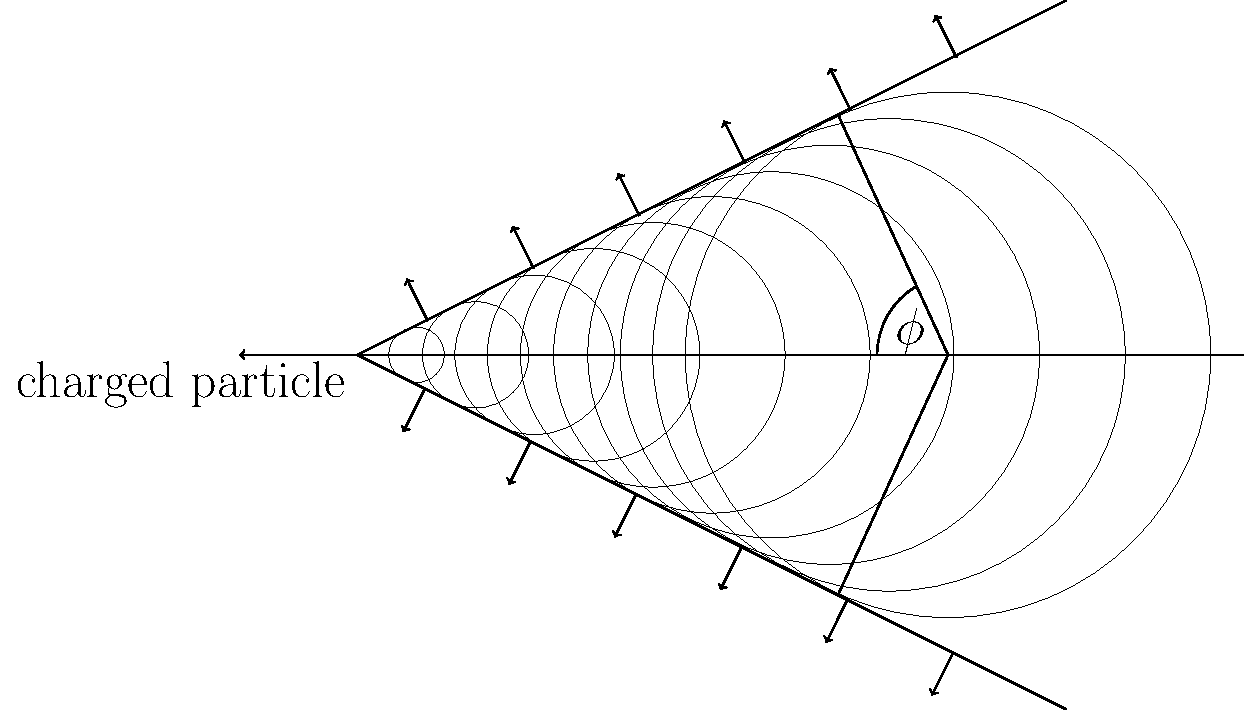
\includegraphics[width=0.5\textwidth]{img/cherenkov}
  \caption{Visualization of the \textit{Cherenkov cone}: A charged particle moves through a medium with a velocity $v>c'$ greater than the phase velocity $c'$ of light within this medium. Due to non-isotropic polarization effects, \textit{Cherenkov photons} are emitted under an angle $\phi$ relative of the direction of motion of the charged particle.}
  \label{fig:ehai2Ahj}
\end{figure}

The spectral distribution of Cherenkov photons is given by equation
\ref{eq:cherenkovspectrum}. A particle with \(\pm z\) elementary charges
that travels a distance \(\d x\) emits \(\d^2 N\) Cherenkov photons with
a wavelength range of \([\nu; \nu + \d\nu]\). \(\alpha\) is the fine
structure constant. \cite{katz2012} The spectrum prefers photons with
shorter wavelengths \(\nu\).

\begin{equation}
  \frac{\d^2 N}{\d x\,\d\nu} = \frac{2\pi\,\alpha\,z^2}{\nu^2}\cdot
  \left( 1 - \frac{1}{\beta^2\,n^2} \right)
  \label{eq:cherenkovspectrum}
\end{equation}

Per GeV of secondary particle shower energy within the detector, an
order of \(10^5\)\nbsp visible Cherenkov photons are created.
\cite{instrumentation}

\subsection{Photon Absorption and Scattering}
\label{sec:scattering}

The propagation of light through a medium depends on the optical
properties of that medium, in particular the velocity of light within
that medium, the scattering probability and the absorption probability.
\cite{lundberg}

The absorption of light for the relevant wavelength range is caused by
electronic and molecular excitation processes \cite{lundberg} and is
quantified by the \textbf{absorption length} \(\lambda\abs\), which is
the mean of the exponentially distributed free path length to absorption
\cite{lundberg}. Therefore, in accordance with the
\noun{Beer-Lambert law}, the absorption length is the path length that
light needs to travel within a medium to have its intensity drop to
\(\sfrac{1}{\e}\) of its original intensity. \cite{lexikonderphysik}
Absorption lengths in the South-Polar ice vary between \(10\m\) in dusty
regions and \(280\m\) in very clear ice layers.
\cite{ackermann, ppcpaper, icepaper}

The scattering of light off microscopic scattering centers, such as
sub-millimeter-sized air bubbles and micron-sized dust grains
\cite{Price1997, ackermann} is the dominant scattering mechanism in
glacial ice \cite{Askebjer1997, lundberg}. This scattering can be
modeled using the more general \noun{Mie scattering} theory, which
describes the scattering of electromagnetic radiation off small,
spherical masses of material with refractive indices differing from the
refractive index of its surroundings.
\cite{Mie1908, ackermann, lundberg}

\noun{Mie scattering} gives the distribution of the scattering angle
\(\theta\) for any wavelength and scattering center size. For ice, this
distribution is approximated using a one-parameter
\noun{Henyey-Greenstein} (HG) phase function
\(p_\text{HG}(\theta; \tau)\), where the one parameter \(\tau\) is the
mean cosine of the scattering angle. \cite{lundberg}

\[ p_\text{HG}(\theta; \tau) = \frac{1 - \tau^2}{2(1 + \tau^2 - 2\tau\, \cos \theta)^\frac{3}{2}}, \ \ \ \tau = \meancostheta \]

The South-Polar ice has shown to be preferentially forward scattering
with a mean cosine of the scattering angle of \(\meancostheta = 0.94\)
with only a weak dependence on the wavelength. \cite{ackermann}

The \textbf{scattering length} \(\lambda\sca\), which is also called
\textbf{geometric} scattering length, is the mean of the exponentially
distributed free path and thereby the average distance between
scatterings. \cite{ackermann} A related and often used quantity is the
\textbf{effective scattering length} \(\lambda\esca\), which is the
distance that light needs to propagate through a turbid medium before
the photon directions are completely randomized. \cite{lundberg}

\begin{equation}
  \lambda\esca = \frac{\lambda\sca}{1 - \meancostheta}
\end{equation}

In a medium with isotropic scattering, the geometric and the effective
scattering lengths are the same. In a preferentially forward scattering
medium like the South-Polar ice, the original direction of a sample of
photons is tendentially retained for several scattering steps until the
photon direction of the sample is isotropized. The projection of the net
velocity vector on the original direction is decreased on average by
\(\meancostheta\) for each scattering. \cite{lundberg}

After \(n\) scatterings, the effectively transported forward distance
along the original direction is
\(\lambda\sca\,\sum_{i=0}^n \meancostheta^i\), such that in the limit of
many scatterings, \(n \rightarrow \infty\), the effectively transported
forward distance becomes the effective scattering length.
\cite{lundberg, ackermann}

\[ \lim_{n \rightarrow \infty} \lambda\sca\,\sum_{i=0}^n \meancostheta^i = \frac{\lambda\sca}{1 - \meancostheta} = \lambda\esca \]

Typical effective scattering lengths within the South-Polar ice are on
the order of \(25\m\) \cite{lundberg} and range from \(5\m\) to \(90\m\)
in the detector volume \cite{icepaper}, corresponding to the geometric
scattering length ranging from \(0.3\m\) to \(5.4\m\).

Light interference effects are ignored during photon propagation as the
average distance between the scattering centers is large compared to the
photon wavelength. \cite{ackermann} Also, despite modeling different ice
regions with abrupt boundaries in the simulations of this study, the
physical boundaries are assumed such that refractive index variations
are continuous. Hence reflection at the medium boundaries is ignored in
simulations. \cite{lundberg}

  \section{Experimental Concepts}
\label{sec:experimental_background}

\subsection{\icecube Detector}

The \icecube neutrino detector is built into a cubic-kilometer of the
glacial ice at Earth's South Pole. 5160 photo detecting optical modules
have been deployed between \(1450\m\) and \(2450\m\) below the surface.
Construction has begun in 2005 with the deployment of the first optical
modules. The detector is fully operational since 2010.
\cite{instrumentation}

The optical modules are anchored on 86 vertical cables called
\textit{strings}, which are positioned on a triangular grid with an
overall hexagonal footprint. The strings are about \(125\m\) apart. Each
string holds 60 optical modules with a vertical spacing of \(17\m\).
\cite{instrumentation}

\begin{figure}[htbp]
  \smallerimage{icecube-schematics-instrumentation}
  \caption{Schematic overview of the \icecube detector. Image source: \cite{instrumentation}}
  \label{fig:aiThai0e}
\end{figure}

Additional to this \textit{in-ice array}, which is designed to measure
neutrinos with energies from the TeV to the PeV scale, the
\textit{DeepCore} sub array hold additional optical modules in order to
lower the detection energy threshold in this region of the detector to
detect neutrinos with energies from \(10\GeV\) to \(100\GeV\).
\cite{instrumentation}

\subsection{Digital Optical Modules (DOMs)}
\label{sec:doms}

The basic detection unit in \icecube is the
\textit{Digital Optical Module} (DOM). Its main components are a photo
multiplier tube (PMT), which detects impacting photons, a main
electronics board, and a flasher board containing light-emitting diodes
(LEDs) for calibration purposes (figure \ref{fig:aK4raigh} a). The DOM's
components are contained within a glass sphere with an outer diameter of
about \(35\cm\) that can withstand high pressures (figure
\ref{fig:aK4raigh} b). The space in between is filled with a gel to
avoid optical effects at the medium boundaries. \cite{instrumentation}

\begin{figure}[htbp]
  \subcaptionbox{Components of the optical module. Image source: \cite{instrumentation}}{\halfimage{dom-components-instrumentation}}\hfill
  \subcaptionbox{Glass sphere containing the components of the optical module. Image source: \cite{gallerynoharness}}{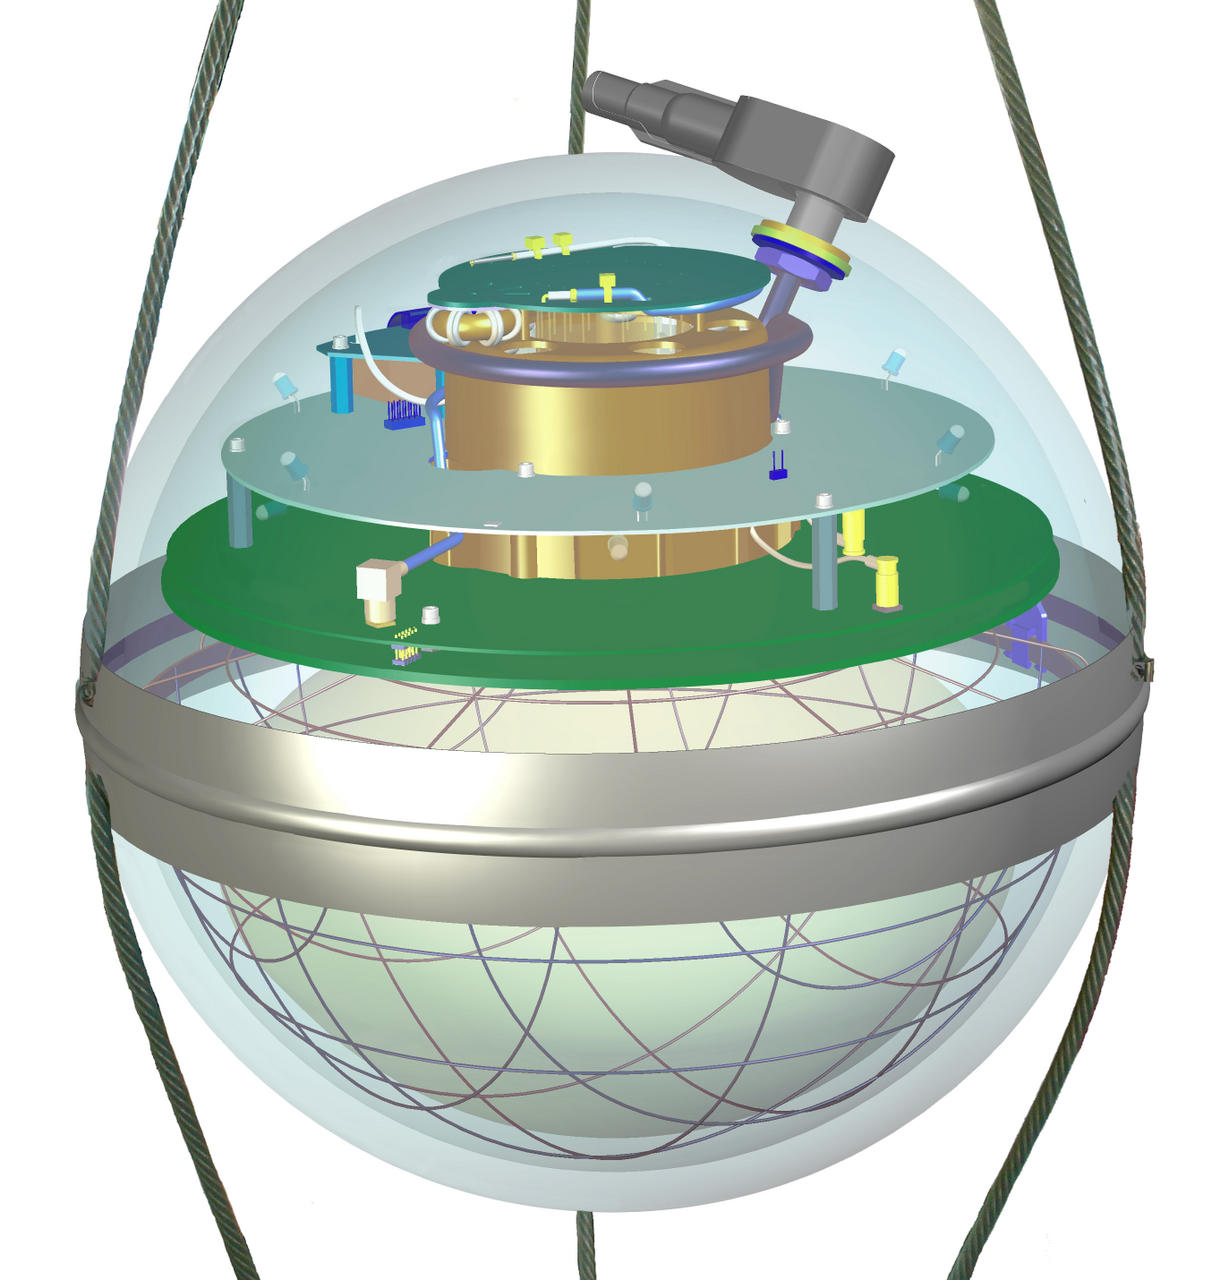
\includegraphics[width=0.35\textwidth]{img/DOMNoHarnessWhiteback_lg-gallery-2013}}
  \caption{Schematic display of a digital optical module (DOM), \icecube's basic detection unit.}
  \label{fig:aK4raigh}
\end{figure}

The recorded signals from the PMT are digitized within the module before
sending the signal to the surface in order to minimize the loss of
information from degradation of analog signals sent over long distances.
\cite{firstyearperformance}

The optical modules are optimized for detecting Cherenkov light emitted
by particles with energies from \(10\GeV\) to \(10\PeV\) up to \(500\m\)
away from the optical module. \cite{instrumentation}

\subsection{Properties of South-Polar Ice}
\label{sec:ice}

The ice at the South Pole has exceptional optical properties, because
air bubbles shrink and vanish under large pressure, forming a so-called
\textit{clathrate hydrate}, where impurities are enclosed inside the ice
crystal structure. \cite{rongenswedishcamera}

Using \icecube's LED flasher calibration system, the properties of
\icecube's glacial ice have been measured: The average distance to
absorption, \(\lambda\abs\), the average distance between successive
scatters \(\lambda\sca\), and the angular distribution of the new
direction after scattering.

To fit these parameters for different depths, the ice has been divided
into \(z\)-layers of an arbitrary thickness of \(10\m\). The ice
parameters have been fitted for each layer such that the properties are
best interpreted as average of their true values over the thickness of
the ice layers. \cite{icepaper}

\paragraph{Scattering}

The measured effective scattering lengths \(\lambda\esca\) range from
\(5\m\) to \(90\m\), corresponding to the geometric scattering length
ranging from \(0.3\m\) to \(5.4\m\). The depth dependence of the
scattering length is shown in figure \ref{fig:Ahxobai3} (a).
\cite{icepaper}

\begin{figure}[htbp]
  \subcaptionbox{Depth dependence of the effective scattering length~$\lambda\esca$ and the effective scattering coefficient~$b_\text{e}:=\sfrac{1}{\lambda\esca}$.}{\halfimage{icepaper-fig-16-esca}\vspace*{2mm}}\hfill
  \subcaptionbox{Depth dependence of the absorption length~$\lambda\abs$ and the absorption coefficient~$a:= \sfrac{1}{\lambda\abs}$.}{\halfimage{icepaper-fig-16-abs}}
  \caption{Values of the absorption length $\lambda\abs$ and the effective scattering length $\lambda\esca$ for different depths, but for a fixed photon wavelength of $400\nm$. Plot taken from \cite[figure 16]{icepaper}. A detailed data table is given in \cite[table C1]{icepaper}.}
  \label{fig:Ahxobai3}
\end{figure}

The wavelength dependence is given by equation \ref{eq:escawavelength}
\cite[section 4]{icepaper}, where
\(b_\text{e} := \sfrac{1}{\lambda\esca}\) is the effective scattering
coefficient, \(\nu\) the photon wavelength, and \(\alpha\) a global fit
parameter. \(b_\text{e}(\nu = 400\nm)\) is given by figure
\ref{fig:Ahxobai3} (a) and \cite[table C4]{icepaper}. The global
parameter \(\alpha\) has been fitted to \(\alpha = 0.90 \pm 0.03\)
\cite[section 5.1]{ackermann}.

\begin{equation}
  b_\text{e}(\nu) = b_\text{e}(\nu = 400\nm) \cdot \left(\frac{\nu}{400\nm}\right)^{-\alpha}
  \label{eq:escawavelength}
\end{equation}

The scattering prefers the forward direction, with a mean cosine of the
scattering angle of \(\meancostheta = 0.94\)
\cite[paragraph 9]{ackermann} (or \(\meancostheta = 0.90\)
\cite{icepaper}).

\paragraph{Absorption}

The absorption lengths in the South-Polar ice vary between \(10\m\) in
dusty regions and \(280\m\) in very clear ice layers. Their depth
dependence is given in figure \ref{fig:Ahxobai3} (b). The absorption
length, which is governed by the dust concentration, is especially low
in the so-called ``dust peak'' at a depth of about \(2000\m\).
\cite{ackermann, ppcpaper, icepaper}

The dependence of the absorption coefficient
\(a := \sfrac{1}{\lambda\abs}\) on the photon wavelength \(\nu\), the
temperature difference \(\delta\tau\) is given by equation
\ref{eq:abswavelength} \cite{icepaper}.

\begin{equation}
  a(\nu) = a_\text{dust}(\nu) + A\,\e^{-\sfrac{B}{\nu}}\, (1 + 0.01 \cdot \delta\tau)
  \label{eq:abswavelength}
\end{equation}\begin{equation}
  a_\text{dust}(\nu) = a_\text{dust}(\nu = 400\nm) \left(\frac{\nu}{400\nm}\right)^{-\kappa}
\end{equation}

The global parameters have been fitted to \(A = (6954 \pm 973)\m^{-1}\),
\(B = (6618 \pm 71)\nm\), and \(\kappa = 1.08 \pm 0.01\)
\cite[section 5.2]{ackermann}.\footnote{The quantity $A$ in \cite{icepaper} corresponds to the quantity $A_\text{IR}$ in \cite{ackermann}. $B$ in \cite{icepaper} corresponds to $\lambda_0$ in \cite{ackermann}.}
The temperature difference \(\delta\tau(d) = T(d) - T(1730\m)\) for
depths \(d\) is given by equation \ref{eq:temperature} \cite{icepaper}.

\begin{equation}
  T(d) = 221.5\unit{K} - 0.00045319\,\frac{\text{K}}{\text{m}}\cdot d + 5.822 \cdot 10^{-6}\,\frac{\text{K}}{\text{m}^2} \cdot d^2
  \label{eq:temperature}
\end{equation}

\paragraph{Ice-Layer Tilt and Ice Anisotropy}

The absorption properties of the ice layers follow the dust
concentration, which does not strictly follow the arbitrary
\(z\)-layers, but is tilted. To model this feature, the ice layers can
also be considered tilted by using an effective-\(z\) coordinate,
\(z_\text{e}(x,y,z) = z + \text{relief}(x,y,z)\), which is shown in
figure \ref{fig:wohr8uaY}. \cite{icepaper}

\begin{figure}[htbp]
  \centering
  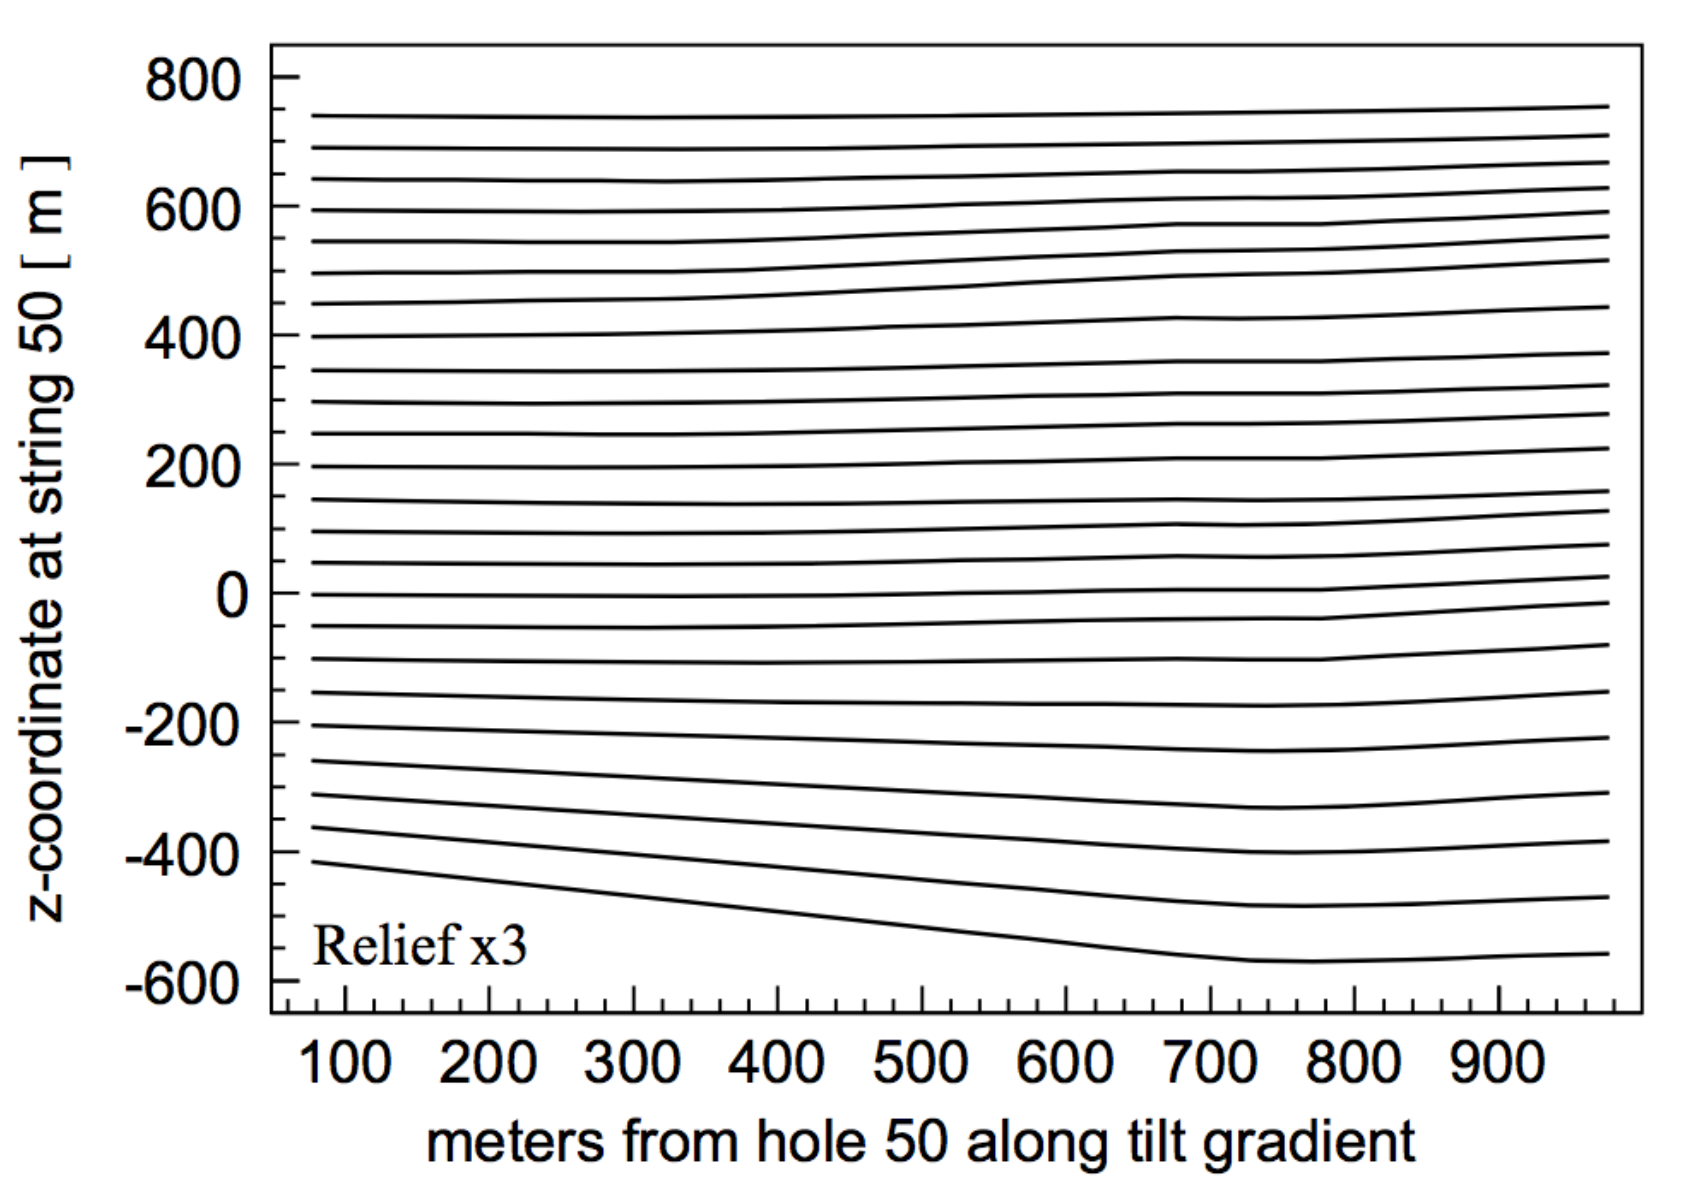
\includegraphics[width=0.5\textwidth]{img/icepaper-fig-14-layers}
  \caption{Ice layers along the average gradient direction within the ice. The relief is amplified by a factor of 3 to enhance the clarity of the layer structure. The lowest layer shown exhibits a shift of $56\m$ between its shallowest and deepest points, which is the largest shift of all layers shown in the figure. Plot and caption taken from \cite[figure 14]{icepaper}.}
  \label{fig:wohr8uaY}
\end{figure}

Furthermore, scattering and absorption show also a slight dependency on
the propagation direction of the photons, aligned with the ice flow
direction of the glacier \cite{icrc17pocam}, which is referred to as
\textit{ice anisotropy}.

This study considers the dependencies of scattering and absorption
length on depth, temperature and wavelength, but does not consider the
ice-layer tilt and the ice anisotropy.

An overview of the different ice models used in \icecube is given in
\cite{flasherdataderivedicemodels}.

\subsection{Hole Ice Around the Detector Strings}
\label{sec:hole_ice}

The so-called \textit{hole ice} is the refrozen water within the drill
holes that were necessary to deploy the detector strings with the
optical modules.

For the \icecube detector, 68 boreholes with an approximate diameter of
\(60\cm\) to a depth of about \(2500\m\) were created using a
\textit{hot-water drilling} technique. Drilling one hole required about
48 hours time. During the deployment, the drill hole was filled with
water. \cite{instrumentation}

When the glacial ice in the drill holes became water, the structures
that were responsible for the specific properties of the bulk-ice layers
were destroyed. Thus, the properties of the hole ice are considered
largely independent of those of the surrounding bulk ice. The deployed
instrumentation become frozen in place and optically coupled to the
surrounding ice sheet when the water in the boreholes became ice again.
\cite{instrumentation}

In order to monitor the freeze-in process, a camera system consisting of
two video cameras in separate spheres, each also equipped with four LEDs
and three lasers, has been deployed along one of the detector strings.
The cameras observed that the drill hole became completely refrozen
within 15 days. \cite{instrumentation}

The camera observations suggest two hole-ice components, a clear outer
region, and an inner column of a smaller scattering length and a
diameter of about \(16\cm\) (figure \ref{fig:daeM6yot}).
\cite{rongenswedishcamera,instrumentation}

\begin{figure}[htbp]
  \centering
  \subcaptionbox{}{\thirdimage{camera2010-01}}\hfill
  \subcaptionbox{}{\thirdimage{camera2010-02}}\hfill
  \subcaptionbox{}{\thirdimage{camera2010-03}}\hfill
  \subcaptionbox{}{\thirdimage{camera2010-04}}\hfill
  \subcaptionbox{}{\thirdimage{camera2010-05}}\hfill
  \subcaptionbox{}{\thirdimage{camera2010-06}}\hfill
  \subcaptionbox{}{\halfimage{swedish-camera-downwards}}\hfill
  \subcaptionbox{}{\halfimage{camera2018-01}}\hfill
  \caption{Monitoring the freeze-in process using a camera system deployed within string number 80. The drill hole freezes from outside in as seen in (a) to (f). The final configuration that can still be observed in 2018 as seen in (h) still shows a diffuse column, called \enquote{bubble column}, on the right-hand side of images (g) and (h). Image sources: \cite{icrc17pocam, camera2010, camera2018}}
  \label{fig:daeM6yot}
\end{figure}

The observed freeze-in process from the outside in is consistent with
the model of \textit{cylindrical freezing}, where impurities or air
bubbles are pushed inwards along the freezing boundaries until they
merge in the center. \cite{rongenswedishcamera} After completing the
freeze-in process, no long-term changes have been observed from 2010 to
2018. \cite{instrumentation, camera2010, camera2018}

In this study, when needing to differentiate between the different
components of the hole ice, the outer clear component will be called
\textit{drill-hole ice}, or \textit{drill-hole column}. The inner
component with a shorter scattering length will be called
\textit{bubble column}. Note, however, that there is no established
nomenclature in the context of \icecube publications, yet.

In this study, the hole-ice columns will be modeled as cylinders. More
complicated geometries such as accounting for the inevitable swinging of
the drilling head, or pressure effects that could lead to a vertical
gradient in the properties of the hole ice, are not considered in this
study.\followup

  \section{Computing Concepts}
\label{sec:simulation_background}

\subsection{Monte-Carlo Simulations of Photons}
\label{sec:monte_carlo}

A Monte-Carlo simulation is a computational method that utilizes a large
amount of random numbers. In order to substitute a complex, possibly
unknown probability distribution, samples of random numbers are drawn
from one or several basic probability distributions and processed in
deterministic calculations. The results are evaluated to gain
information about processes or quantities involved. This method is
especially useful for systems with many degrees of freedom.
\cite{physiklexikon}

This study needs to determine whether and when detector modules are hit
by photons from a given source assuming different ice parameters. In
principle, one could devise a mathematical function of input quantities
and random variables that determines whether and when a photon is
detected by an optical module. This task would be disproportionately
complex, however, especially as the function would have to be revised
for every change in the underlying models.

Therefore, this study uses Monte-Carlo simulations that propagate
photons through the ice in several simulation steps. Based on drawing
random numbers from basic probability distributions, the simulation
determines in each step, whether and when to scatter or to absorb the
photon next, and, in which direction the photon is to be scattered.
Checking for DOM collisions in each step, the simulation is able to
determine for each photon and each detector module whether and when the
photon is detected by the module.

To obtain probability statements from Monte-Carlo simulations, the
\textit{law of large numbers} is employed: If an experiment involving
random processes is repeated \(n\) times, the relative frequency
\(h_n(A):=\sfrac{H(A)}{n}\) of an event\nbsp \(A\), which occurs
\(H(A)\) times in total in these \(n\) experiments, approaches the
\textit{probability}\nbsp \(p(A)\) of the event\nbsp \(A\) for large
numbers\nbsp \(n\) with certainty. \cite{physiklexikon}

\[
  \lim_{n \rightarrow \infty} \text{P}(|h_n(A) - p(A)| < \epsilon) = 1, \ \ \ \epsilon \in \reals
\]

Technical progress concerning computational devices, graphics processing
units (GPUs) in particular, allows to perform highly parallelized
Monte-Carlo simulations on large scale. For a random-walk description of
the propagation of photons, see \cite{absorption1997}. A first
implementation of a photon-propagation simulation through ice is
described in \cite{lundberg}. A study of propagation simulations using
GPUs is presented in \cite{ppcpaper}.

\subsection{Parallel Computing on Graphics Processing Units (GPUs)}
\label{sec:parallel_computing}

Graphics processing units (GPUs) are optimized for performing simple
calculations for a large number of values in parallel.

The general procedure for GPU calculations is to allocate memory on the
GPU, to copy input parameters onto the GPU, perform calculations on the
GPU, and then to download the results from the GPU. This procedure is
efficient if the time that is spent for allocating, and copying to and
from the GPU memory is short compared to the time spent with
calculations on the GPU. \cite{cudacourse}

The basic units for parallelization are \textit{computational threads}.
All operations within a thread are sequential, while all those
operations are applied to a set of threads, called
\textit{thread block}, in parallel. Each GPU may have one or several
thread blocks. \cite{cudacourse}

While technological progress is achieved rapidly, GPU memory is still a
considerably limited resource. In particular fast memory, which requires
a small amount of physical time for reading and writing information, is
expensive. Therefore, memory is divided in several categories: The
\textit{local memory} that belongs only to one thread, is fastest but
most limited. The \textit{shared memory}, which is common to all threads
of one thread block, is slower. Next slower is the
\textit{global memory}, which is common to all thread blocks on the GPU.
Slowest, but in comparison to the GPU memory practically unlimited, is
the \textit{host memory}, which is memory not on the GPU but on other
components of the computer. Efficient memory use is one of the key
concepts for performant GPU programming.
\textit{Coalesce memory access}, which means that each thread in a
thread block reads or writes from or to a coherent memory block parallel
to the other threads of the thread block, increases memory access
performance. \cite{cudacourse}

Techniques that utilize the internal optimizations of GPUs allow for
further performance improvements: Using GPU-native
\textit{atomic operations} such as the increment operator that increases
the value of a variable by 1 is more performant than using a generic
mathematical operation. GPUs support vectors with four components as
native data types. Using \textit{native vectorial operations} such as a
dot product is more performant than implementing the operation as
mathematical function manually. \cite{cudacourse}

In parallel computing, the \textit{step complexity} of an algorithm is a
measure of the physical time the parallelized algorithm needs to run.
The \textit{work complexity} is a measure for the summed computational
work that is done by all threads in that time. A pattern to avoid in
this context is \textit{thread divergence} where some threads have to
stay idle and wait for other threads completing their work.
\cite{cudacourse}


  % Methods:
  % Everything needed to reproduce the work
  \section{Development of Algorithms For the Direct Photon-Propagation Through Hole Ice With \clsim}
\label{sec:methods}

\renewcommand\currentsection{Hole-Ice Algorithms}

\subsection{Modeling Hole Ice as Distinct Cylindrical Ice Volumes}

In the \icecube simulation framework, photon propagation simulation
takes several dependencies into account: The photon absorption length
and the photon scattering length may depend on the photon's wavelength.
Absorption and scattering length may also depend on the photon's
\(z\)-coordinate as the South-Polar ice consists of several
\textit{ice layers}. These ice layers may also be tilted. Furthermore,
the absorption length may depend on the photon's direction of motion,
which is called \textit{absorption anisotropy}.

This study adds another ice feature to the simulation: Hole ice may be
modeled by adding cylinder-shaped volumes within the surrounding bulk
ice where the propagation properties, or, to be specific, the photon's
absorption length and scattering length, differ from the propagation
properties of the bulk ice.

Figure \ref{fig:aiw2Thah} illustrates such a scenario for one single
photon: The photon's trajectory starts in the bulk ice. The photon
enters the hole-ice cylinder where the scattering length is shorter as
in the bulk ice. Hence the photon scatters more frequently within the
cylinder. When the photon leaves the hole-ice cylinder the propagation
properties of the bulk ice take effect again, resulting in the photon
scattering less frequently after leaving the cylinder.

\begin{figure}[htb]
  \centering
  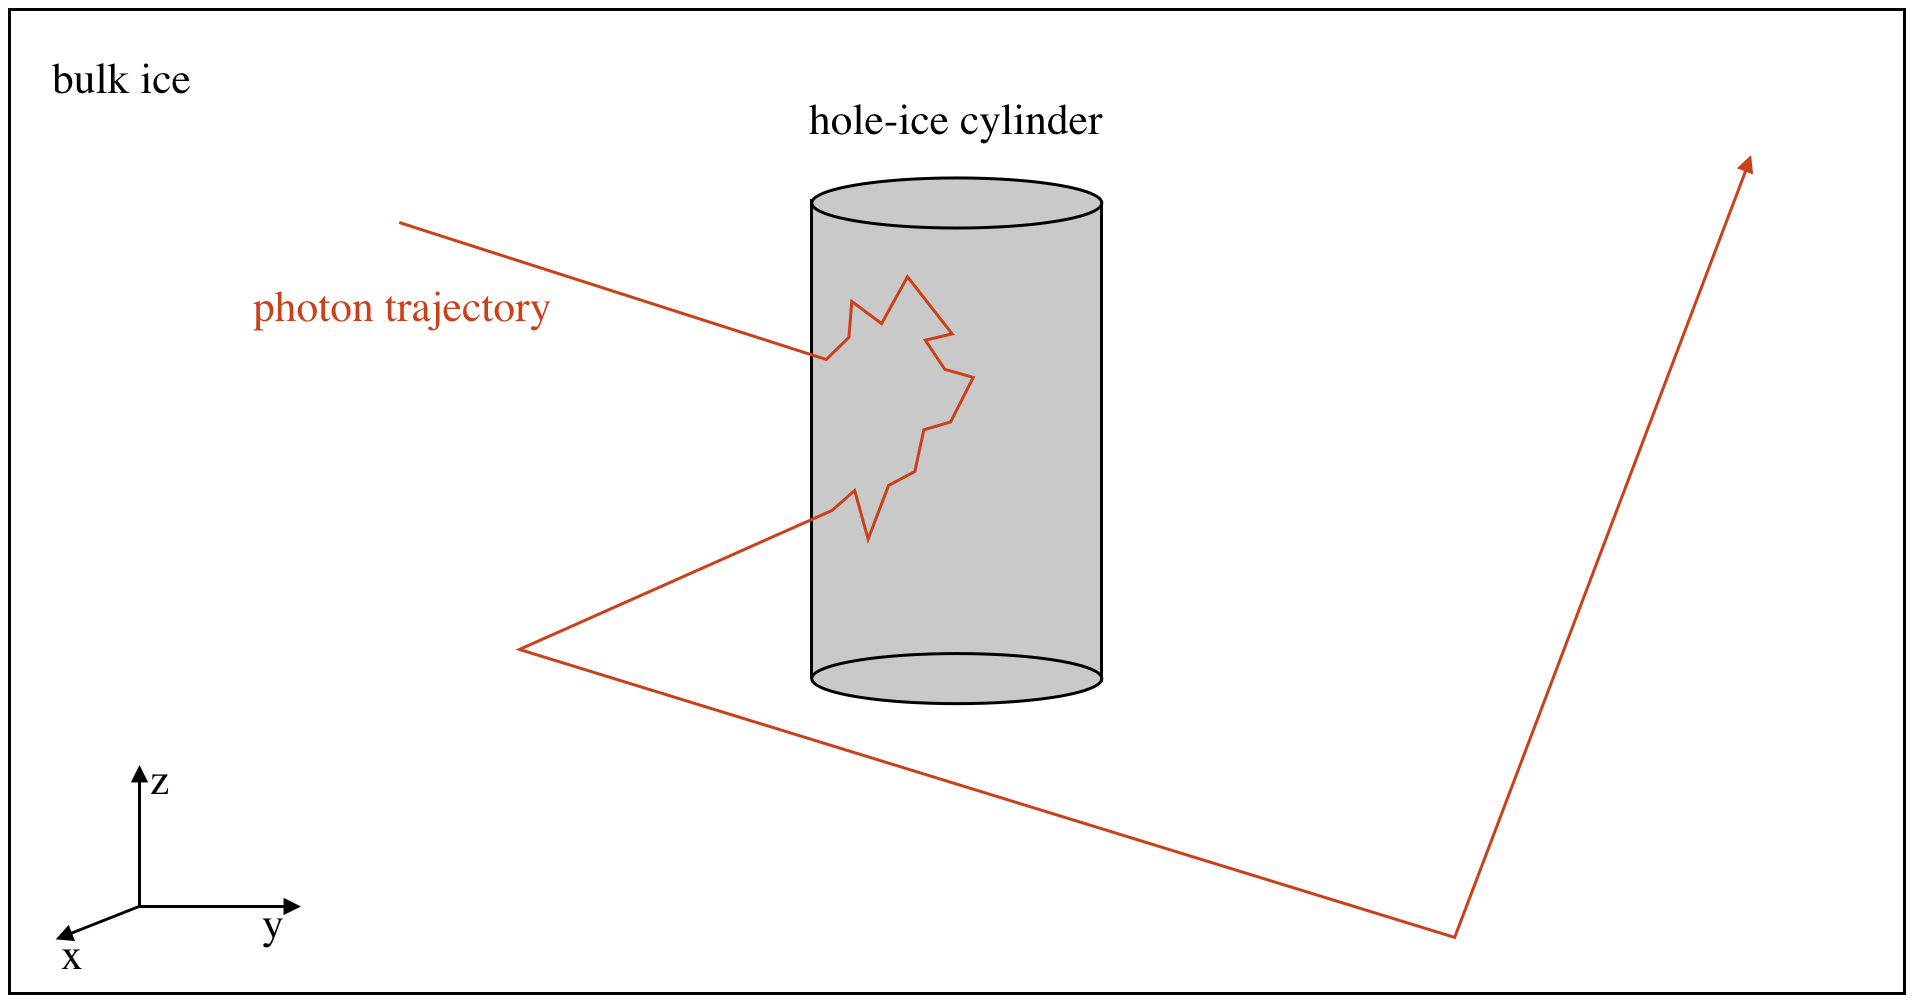
\includegraphics[width=0.6\textwidth]{img/hole-ice-as-cylinder-shaped-areas}
  \caption{Schematic diagram of a propagating photon. The photon enters a hole-ice cylinder with a scattering length different from the outside ice. When leaving the cylinder the photon assumes the scattering length of the outside ice again.}
  \label{fig:aiw2Thah}
\end{figure}

In this study, cylinders are always defined along the \(z\)-axis. Also,
the scattering angle is assumed to behave the same within the hole ice
as in the bulk ice.

  \subsection{Propagating Photons Through Different Media}

\subsubsection{Very Basic Photon-Propagation Algorithm}

A first, very basic photon-propagation algorithm, which is not actually
implemented in \clsim, but is presented as comparative example, moves
the photon by a small distance \(\delta x\). At the new photon position,
the algorithm checks for detection at an optical module and randomizes
as a function of the scattering and absorption lengths whether the
photon should be scattered or absorbed by the ice at this position.
Then, the photon is propagated again by the same small distance
\(\delta x\). The same loop repeats until the photon either hits an
optical module or is absorbed by the ice. Figure \ref{fig:ieph6Bie}
illustrates a propagation scenario in a two-dimensional coordinate
system. Figure \ref{fig:ohsa0miG} presents the algorithm as flow chart.

\begin{figure}[htb]
  \smallerimage{photon-trajectory-naive-ieph6Bie}
  \caption{Illustration of a basic photon-propagation algorithm in a two-dimensional coordinate system. The photon is propagated by a small distance in each propagation step. At each position, the algorithm checks for absorption, scattering and whether an optical module has been hit.}
  \label{fig:ieph6Bie}
\end{figure}

\begin{figure}[p]
  \image{algorithm-naive-propagation}
  \caption{Flow chart of a basic photon-propagation algorithm. Interfaces, where the algorithm begins or ends, are displayed as violet pill shapes. Processes, where the algorithm performs an operation or a calculation, are displayed as brown rounded boxes. Decisions are displayed as green rounded diamond shapes. One propagation step consists of moving the photon by a fixed small distance $\delta x$, checking for detection as well as randomizing scattering and absorption within the ice.}
  \label{fig:ohsa0miG}
\end{figure}

This very basic propagation algorithm can handle propagation through
different media just by making the scattering and absorption
probabilities depend on the current photon position and direction. Ice
layers and ice layer tilt can be implemented by making the scattering
and absorption probabilities depend on the current photon position,
absorption anisotropy by making the absorption probability depend on the
current photon direction as well. Hole-ice cylinders can be implemented
by checking whether the current photon position is within any of a list
of cylinders defined in any way, either by supplying a list of cylinder
coordinates and radii, or by re-using the coordinates of the detector
strings.

This basic propagation algorithm, however, is very inefficient regarding
computational performance: The algorithm moves the photon over long
distances in small steps without changing the direction. For a typical
geometric scattering length of two meters, moving the photon in steps of
\(\delta x = 1\mm\) per propagation step would mean performing 2000
propagation steps before changing the direction of motion.

The propagation algorithm can be made more efficient by moving the
photon in each propagation step not by a small distance \(\delta x\) but
by the whole distance to the next interaction point. This way, the above
example would take only one propagation step rather than 2000. This
performance improvement, however, comes at the cost that propagating
through different media requires a different, more involved
computational approach. This more efficient propagation algorithm, which
is the standard photon-propagation algorithm in \icecube, will be
described in the next section.

\subsubsection{Standard Photon Propagation Algorithm}
\label{sec:standardphotonpropagationalgorithm}

\label{sec:standard_photon_propagation_algorithm}
\label{sec:standard_clsim}

In \icecube's standard photon-propagation algorithm, a propagation step
moves the photon not just by a small, fixed distance \(\delta x\) but to
the next interaction point at once. An interaction may be the photon
scattering within the ice, the photon being absorbed by the ice, or the
photon hitting an optical module. \cite{clsimsource, ppcpaper}

At each scattering point, the algorithm randomizes the new photon
direction based on the scattering angle distribution, and how far the
photon will travel until it is scattered again based on the scattering
length. How far the photon will travel until it is absorbed is
randomized just once when the photon is created.

For each propagation step, the algorithm checks whether the photon will
hit an optical module on the path between two scattering points. Also,
the algorithm checks whether the destined distance to absorption will be
reached before the next scattering point. If the photon will be
destroyed in this step, either by being absorbed in the ice, or by
hitting an optical module, the final position is recorded. Otherwise,
the photon proceeds to the next scattering position. This loop is
repeated until the photon is either absorbed or hits an optical module.
\cite{ppcpaper}

Figure \ref{fig:Ar0vai8u} shows a flow chart of this algorithm. Figure
\ref{fig:oheeL3ai} shows the same two-dimensional scenario as figure
\ref{fig:ieph6Bie} in the previous section, but illustrates how the same
photon trajectory is modeled by this algorithm with significantly less
simulation steps.

\begin{figure}[htbp]
  \smallerimage{photon-trajectory-oheeL3ai}
  \caption{Illustration of \icecube's standard photon-propagation algorithm in a two-dimensional coordinate system. The photon is propagated from one scattering point to the next scattering point in each propagation step. In each step, the algorithm checks for absorption and whether an optical module (DOM) is hit in between the two scattering points.}
  \label{fig:oheeL3ai}
\end{figure}

\begin{figure}[p]
  \image{algorithm-photon-propagation}
  \caption{Flow chart of the standard photon-propagation algorithm. One propagation step consists of moving the photon from one scattering point to the next scattering point. If the photon hits an optical module in between the two scattering points, the algorithm records a hit and destroys the photon. If the photon is absorbed in the ice in between the two scattering points, it will only be propagated to the position of absorption and it will not reach the next scattering point. When adding propagation through hole ice with a different scattering length to this algorithm, the calculation of the next scattering point needs to be modified accordingly.}
  \label{fig:Ar0vai8u}
\end{figure}

Assuming the number of calculations in each scattering step is of the
same order of magnitude in both described algorithms, the number of
simulation steps translates to the total number of calculations the
processing unit needs to perform for each photon. Thus, the algorithm
that needs much less simulation steps is also much more efficient.

Propagating a photon through several media with different optical
properties is more involved in this algorithm than in the basic one. If
the algorithm calculates the distance to the next interaction point
considering only the interaction properties of the ice at the current
position of the photon as suggested by the basic algorithm, then the
next interaction point would be calculated inaccurately if the medium
properties change between two interaction points. The larger the
scattering length gets compared to the size of the ice volumes with
constant interaction properties, the worse the inaccuracies become. This
can be illustrated by an extreme example where the scattering length and
the absorption length within the bulk ice are several meters long, but
the photon would hit a cable with a diameter of only a couple of
centimeters between two scattering points. The cable would absorb the
photon at once. But if the next interaction point is calculated
evaluating only the interaction properties at the position of the
current scattering point, then the photon ignores the cable and
continues on its path without being absorbed by the cable.

The solution to this problem chosen for the standard propagation
algorithm in \icecube is to implement medium transitions in the
following manner: Rather than randomizing the geometrical distance
\(X:=\overline{AB}\) from the current interaction point \(A\) to the
next interaction point \(B\) itself, the algorithm randomizes the number
\(N :\in \reals^+\) of interaction lengths the photon will travel to the
interaction point, like a budget. This budget is spent by considering
the different media on the way from the current interaction point along
the photon's direction, and converting the number of interaction lengths
into a geometrical distance according to the shares of the different
media in the path of the photon between the two interaction points.

Suppose, starting at interaction point \(A\), the photon travels in
\(m :\in \naturals\) media \(M_i\) with interaction lengths
\(\lambda_i\) for a distance of \(x_i\) respectively until it reaches
the next interaction point \(B\). In each medium \(M_i\), the algorithm
spends \(n_i: x_i = n_i\,\lambda_i\) of the budget \(N:=\sum_1^m n_i\)
that has been randomized at interaction point \(A\) until it reaches
interaction point \(B\) in a distance \(X:=\overline{AB}\).

\begin{equation}
  X = \sum_{i=1}^m x_i = \sum_{i=1}^m n_i\,\lambda_i, \ \ \ \ N = \sum_{i=1}^m n_i
  \label{eq:convertbudgettodistance}
\end{equation}

Each distance \(x_i\) is the length of the trajectory the photon spends
in medium \(M_i\). The first distance \(x_1\) is the distance from the
starting point \(A\) to the medium border of \(M_1\) and \(M_2\) along
the photon direction. The subsequent distances \(x_i\) are the distances
of the first medium border (of \(M_{i-1}\) and \(M_i\)) and the second
medium border (of \(M_i\) and \(M_{i+1}\)) respectively along the photon
direction. The last distance \(x_m\) is determined by how much of the
budget \(N\) is left in the last medium, \(x_m = n_m\,\lambda_m\), such
that the overall budget \(N:=\sum_{i=1}^m n_i\) is spent.

Coming back to the extreme example where a cable lies ahead on the
photon path, the algorithm now considers all media on the path along the
photon direction in order to convert the number of interaction lengths
into a geometrical distance to the interaction point. As the absorption
length within the cable's medium is set to zero, all of the
absorption-length budget is spent at the medium border to the cable,
resulting in the final interaction point of the photon being right at
the point where the photon enters the cable. Thus, this algorithm lets
the photon be absorbed by the cable as intended.

Ice layers, the tilt of the ice layers, and the absorption anisotropy
are modeled in this algorithm by implementing the rules on how the
interaction budget is spent accordingly. Adding cylinder-shaped volumes
to model hole ice or cables means to further extend these rules on how
the scattering and absorption budgets are spent along the photon's
trajectory.

Two different algorithms for the photon propagation through
cylinder-shaped volumes are described in the following sections: Section
\ref{sec:algorithm_a} describes a first approach where the propagation
through the hole-ice cylinders is added as subsequent correction for the
existing medium-propagation algorithm. Section \ref{sec:algorithm_b}
describes a second approach where the existing medium-propagation
algorithm is rewritten in order to support the propagation through
hole-ice cylinders the same way as other medium transitions.

  \label{sec:tools}

\subsection{\icecube Simulation Framework}

This study uses the \noun{IceCube Simulation Framework}, short \icesim,
in Version \texttt{V05-00-07}. The framework, written in
\noun{C++}\footnote{C++ programming language, \url{https://isocpp.org}}
and
\noun{Python}\footnote{Python programming language, \url{https://www.python.org}},
provides the software needed to run simulations, to write and to process
\icecube-specific data such as simulated or recorded events and the
detector geometry.

\docframe{
\docparwithoutframe{The documentation of the \noun{IceCube Simulation Framework} can be found at \url{http://software.icecube.wisc.edu/documentation/}.}\medskip

\docparwithoutframe{A guide on how to install the \noun{IceCube Simulation Framework} with all the other tools needed for this study is provided at \url{https://github.com/fiedl/hole-ice-study/blob/master/notes/2018-01-23_Installing_IceSim_in_Zeuthen.md}.}\medskip

\sourceparwithoutframe{The source code of the \noun{IceCube Simulation Framework} can be found at \url{http://code.icecube.wisc.edu/projects/icecube/browser/IceCube/meta-projects/simulation}.}
}

\subsection{Photon Propagation With \clsim}

The main tool of this study is the photon-tracking simulation software
\clsim. This software implements a ray-tracing algorithm described in
section \ref{sec:standardphotonpropagationalgorithm}, modeling
scattering and absorption of light in the deep-glacial ice at the South
Pole or in Mediterranean sea water. \cite{clsimreadme} Written in C++,
\noun{Python} and
\noun{OpenCL C}\footnote{OpenCL, Open Computing Language, \url{https://www.khronos.org/opencl}},
\clsim uses \noun{OpenCL} to simulate the photon propagation in a highly
parallelized way on graphics processing units (GPUs). \cite{clsimsource}
\clsim reads the photon sources from the \icesim data, converts the data
into a format that can be used on GPUs, uploads the data and the
propagation program (``kernel'') onto the GPU, and propagates the
photons there. Then \clsim downloads the hits and tracks of the
propagated photons, performs post-processing operations such as
accepting hits on optical modules based on the acceptance criteria of
the modules, and converts them back into an \icesim-compatible format.

\docframe{
\sourceparwithoutframe{The source code of \clsim, which is released under the Internet Systems Consortium (ISC) license, can be accessed at the \clsim code repository \url{https://github.com/claudiok/clsim}.}\medskip

\sourceparwithoutframe{In order to simulate the propagation through hole ice, \clsim has been modified for this study. Until the modified source code has been merged into the main code repository, the modified \clsim source code can be accessed through the forked code repository at \url{https://github.com/fiedl/clsim}.}\medskip

\docparwithoutframe{A guide on how to install the modified version of \clsim can be found in appendix \ref{sec:howtoclsim} and on \url{https://github.com/fiedl/hole-ice-study/blob/master/notes/2018-01-23_Installing_IceSim_in_Zeuthen.md\#install-patched-clsim}.}
}

\subsection{Photon Visualization With \steamshovel}

\steamshovel (Figure \ref{fig:steamshovel}) is the event and data viewer
software of \icecube. It allows to visualize the \icecube detector as
well as events that have been recorded, reconstructed or simulated in
the detector. For example, \steamshovel can be used to visualize light
sources such as muons traveling through the detector producing Cherenkov
light, or LED flashes that can be emitted by the optical modules for
calibration purposes. \steamshovel may also visualize the photons
propagating through the ice, or the amount of light detected by the
optical modules. Data containing timing information can be visualized in
an animated manner, watching an event as slow-motion animation.

\begin{figure}[htbp]
  \image{steamshovel}
  \caption{Screenshot of \steamshovel, the \icecube event and data viewer software. The main workspace shows a schematic of the \icecube detector with its 86 strings holding 60 optical detector modules each. Control elements allow to hide and display components and to navigate through the event information. Image source: \cite{steamshoveldocumentation}}
  \label{fig:steamshovel}
\end{figure}

Most event visualizations in this study are created using \steamshovel.
In order to visualize hole ice and propagating photons for this study,
several patches of the standard \steamshovel code are required.

\sourcepar{The required \steamshovel patches are provided within the code repository of this study: \url{https://github.com/fiedl/hole-ice-study/tree/master/patches/steamshovel}}

\subsection{Other Software Tools}

In order to process data, to perform statistical analyses, and to plot
data, this study uses several supplementary software libraries, such as
\noun{NumPy}\footnote{NumPy package for scientific computing, \url{http://www.numpy.org}},
\noun{Matplotlib}\footnote{Matplotlib plotting library, \url{http://matplotlib.org}}
and
\noun{Pandas}\footnote{Pandas Python Data Analysis Library, \url{http://pandas.pydata.org}}.
For unit tests (section \ref{sec:unit_tests}), this study uses the
\noun{gtest}\footnote{Google Test Framework, gtest, \url{https://github.com/google/googletest}}
testing framework.

\docpar{The necessary scripts and installation instructions can be found in the code repository of this study at \url{https://github.com/fiedl/hole-ice-study}.}

  \subsection{Algorithm A: Hole-Ice Propagation as Subsequent Correction of the Propagation Without Hole Ice}
\label{sec:algorithm_a}

A first approach to adding propagation through hole-ice cylinders to the
standard propagation algorithm (section
\ref{sec:standardphotonpropagationalgorithm}) implemented in \clsim is
to add a subsequent correction to each simulation step without rewriting
the existing algorithm.

\sourcepar{The source code of the implementation of this first approach can be found in appendix \ref{sec:algorithm_a_source}, in the folder \texttt{algorithm\_a} on the CD-ROM, as well as in the code repository at \url{https://github.com/fiedl/clsim/tree/sf/hole-ice-2017/resources/kernels/lib/hole_ice}.}

This approach assumes that the scattering length \(\lambda\hi\sca\) and
the absorption length \(\lambda\hi\abs\) within the hole ice can be
expressed as multiple of the corresponding scattering length
\(\lambda\sca\) and absorption length \(\lambda\abs\) within the
surrounding bulk ice.

\[
  \lambda\sca\hi = f\sca \, \lambda\sca, \ \ \ \lambda\abs\hi = f\abs \, \lambda\abs
\]

The factor \(f\sca :\in \reals^+_0\) will be called
\textbf{scattering length factor}, \(f\abs :\in \reals^+_0\)
\textbf{absorption length factor}. These factors can be implemented as
properties of the individual hole-ice cylinders, or as common property
of all cylinders.

If, for example a cylinder has an absorption length factor of
\(f\abs = 1\), the absorption length within the hole ice is the same as
in the surrounding bulk ice. If the absorption length factor is
\(f\abs = 0\), a photon will be absorbed instantly when entering the
hole-ice cylinder. A scattering factor of \(f\sca=0.1\) means that the
scattering length within the hole ice is one tenth of the scattering
length within the surrounding bulk ice.

\paragraph{Task}

The task of this \textbf{hole-ice-correction algorithm} is to modify the
quantities that are effected by the hole ice in each simulation step.

Figure \ref{fig:Edahi9sh} illustrates this task: The standard
\clsim propagation algorithm calculates the next scattering point \(B\)
without any knowledge of the hole ice. The hole-ice algorithm takes the
properties of the hole ice into account and calculates a correction for
the next scattering point. \clsim will use the corrected next scattering
point \(B'\) rather than the originally calculated point \(B\).

\begin{figure}[htbp]
  \smallerimage{photon-trajectory-Edahi9sh}
  \caption{Illustration of the task of the hole-ice correction algorithm. In this two-dimensional scenario, the hole-ice cylinder is represented by a circle. When the photon scatters at point $A$, the standard-\clsim algorithm calculates the next scattering point $B$ without knowledge of the hole ice. The hole-ice correction algorithm calculates what fraction of the trajectory $AB$ runs through the hole ice and determines a correction, resulting in a hole-ice-corrected next scattering point $B'$.}
  \label{fig:Edahi9sh}
\end{figure}

\paragraph{Context}

The hole-ice-correction algorithm is inserted into the
\clsim propagation algorithm's simulation step right after \clsim has
calculated the distance to the next scattering point and the remaining
distance to the absorption point without knowledge of the hole ice.
After the hole-ice-correction algorithm follows the check whether the
photon hits an optical module on the way from \(A\) to \(B'\).

The hole-ice-correction algorithm takes the following input parameters:
Current photon position at point \(A\), photon direction after
scattering at point \(A\), a list of the hole-ice cylinders with their
coordinates and radii, the hole-ice scattering length factor \(f\sca\)
and absorption length factor \(f\abs\) as common properties of all
hole-ice cylinders, the distance the next scattering point calculated by
the standard algorithm, and the remaining distance to the absorption
point calculated by the standard algorithm. As output parameters, the
hole-ice correction algorithm returns the hole-ice-corrected distance to
the next scattering point and the hole-ice-corrected remaining distance
to the absorption point.

\paragraph{Procedure}

For each propagation from one scattering point \(A\) to the next
scattering point \(B\), the hole-ice algorithm calculates the
intersection points of the photon trajectory \(AB\) and the hole-ice
cylinders in range. Based on what portion of the distance \(AB\) runs
through the hole ice, the algorithm calculates a correction for the
distance to the next scattering point and a correction for the remaining
distance to the absorption point.

Both calculations, scattering correction and absorption correction,
depend on each other: If the photon scatters earlier within the hole ice
than determined by the standard algorithm, then the corrected path
within the hole ice is shorter than the original one, which means that
the remaining distance to the absorption point will be longer as less of
the absorption budget is spent, yet. If, on the other hand, the hole ice
absorbs the photon instantly when entering the cylinder, then the
corrected final position \(B'\) of this simulation step won't be the
point determined by the scattering correction but the point where the
photon enters the cylinder.

Figure \ref{fig:bahxug7O} shows a flow chart of this algorithm including
the loop over the hole-ice cylinders in range, the calculation of the
intersection points of photon path and hole-ice cylinder, the correction
of the next scattering point and the correction of the remaining
distance to absorption.

\begin{figure}[htbp]
  % https://github.com/fiedl/hole-ice-study/issues/77#issuecomment-396559561
  \image{algorithm-hole-ice-2017}
  \caption{Flow chart of the hole-ice-correction algorithm, which calculates subsequent corrections for the quantities that are effected by the hole ice: the distance to the next scattering point and the remaining distance to absorption of the photon. Both corrections depend on each other: If the photon scatters earlier, the absorption correction will be smaller. The algorithm returns the corrected quantities to the standard algorithm, which uses the corrected quantities from that point on.}
  \label{fig:bahxug7O}
\end{figure}

\paragraph{Intersection Calculations}

In order to determine the fraction of the path \(AB\) of the photon that
runs through the hole-ice cylinder, the intersection points of the
photon path and the cylinder need to be calculated. This can either be
done solving the geometric equations coordinate-wise for the coordinates
of the zero, one or two intersection points, or by treating the same
scenario as vectorial problem, calculating the coordinate vectors of the
intersection points using other vectorial quantities rather than
separate coordinates. The latter approach turns out to be more efficient
as it utilizes the support of native vector operations of the graphics
processing units. Both approaches are presented in appendix
\ref{sec:intersections}.

\paragraph{3D-2D Projection}

Intersection points can be calculated in two dimensions by projecting
all coordinates from the three-dimensional coordinate system onto the
\(x\)-\(y\) plane along the \(z\)-axis, and then calculating the
intersection of a line and a circle rather than the intersections of a
line and a cylinder. The fraction of the photon path that runs through
the hole ice is the same as in three dimensions due to the intercept
theorem, because both, the distance to the intersection point,
\(\len{AX}_\text{2D}:=\xi \len{AX}_\text{3D}\), and the distance to the
next scattering point, \(\len{AB}_\text{2D}:=\xi \len{AB}_\text{3D}\),
use the same projection factor \(\xi \in \reals^+\), which itself
depends on the photon direction.

\[
  \frac{\len{AX}_\text{2D}}{\len{AB}_\text{2D}} = \frac{\len{AX}_\text{3D}}{\len{AB}_\text{3D}}
\]

The relative distance corrections, \(\sfrac{\Delta x}{\len{AB}}\), are
the same in two and three dimensions due to the same reason. But the
absolute distance correction
\(\Delta x : \len{AB'} = \len{AB} + \Delta x\) needs to be expressed in
three dimensions when adding the correction to the distances used in the
standard algorithm as they are defined for a three-dimensional
coordinate system. Keeping this conversion requirement in mind, the
geometric cases of the photon path \(AB\) running through a hole-ice
cylinder can be examined in two dimensions.

\paragraph{Geometric Cases}

When the hole-ice algorithm calculates the distance correction
\(\Delta x: \len{AB'} = \len{AB} + \Delta x\), there are several
geometric cases to consider, depending on the number \(N\) of
intersections of the photon path \(AB\) with the hole-ice cylinder and
whether the path starts within the cylinder or outside the cylinder.

\begin{figure}[htbp]
  \smallerimage{intersection-iefai4iV}
  \caption{Intersection of the line along the photon path $AB$ with the hole-ice cylinder in two dimensions, where the cylinder is represented by a circle of radius $r$ around the center $M$. The first intersection point is $Y$, the second intersection point $X$. The second intersection point $X$ is beyond the path's end point $B$. Thus, the number $N$ of intersections is considered to be $N=1$ in this case.}
  \label{fig:iefai4iV}
\end{figure}

The distance correction depends on the fraction \(w :\in \reals^+_0\) of
the path length \(\len{AB}\) that runs within the hole-ice cylinder.

\begin{description}
  \item[Case 1] If the photon starts outside the cylinder and the path has no intersection with the cylinder ($N = 0$), then the path does not run through the cylinder, $w = 0$, and the distance correction $\Delta x$ needs to be zero: $\Delta x = 0$.
  \item[Case 2] If the photon starts inside the cylinder and the path has no intersection with the cylinder ($N = 0$), then the whole path is within the cylinder, $w = 1$. A photon that would travel a distance of $\lambda$ within the bulk ice, travels a distance of $\lambda\hi$ within the hole ice, $\lambda\hi = f\,\lambda$. The distance correction $\Delta x$ for this photon would be $\Delta x = \lambda\hi - \lambda = (f - 1)\lambda$, or more generally, $\Delta x = (f - 1) \len{AB}$.
  \item[Case 3] If the photon starts outside the cylinder, but intersects the cylinder once ($N = 1$), then the first part of the trajectory, $AY$, stays the same, and only the path from the first intersection point $Y$ to the destination point $B$ runs within the hole ice, $w = \len{YB} / \len{AB}$. As only this fraction needs to be corrected, the distance correction is $\Delta x = (f - 1)\len{YB}$.
  \item[Case 4] If the photon intersects the cylinder once ($N = 1$), but starts within the cylinder, only the first part, $AC$, of the path needs to be corrected.

  $C$ is the \textbf{termination point} of the trajectory inside the cylinder. In cases where the photon reaches the far end of the cylinder, $C$ is just the second intersection point, $C = X$. If the trajectory within the cylinder is terminated, however, by the other interaction respectively, for example if the photon is scattered away before reaching the far end when calculating the absorption correction, $C$ is the point where the trajectory is terminated by the other interaction.
    % termination point formalsim: 2017-10-10 2017-10-13 2018-02-02

  In contrast to Case 3 where the outside distance $\len{AY}$ has been fixed, in this case the outside trajectory part $\len{CB}$ comes after the hole-ice part $\len{YC}$ and will be the shorter the stronger the hole-ice correction is. Therefore, one needs to use the scaled distance $\len{AC} / f$ to determine how much of the path will remain outside the cylinder, resulting in a distance correction of $\Delta x = (1 - \frac{1}{f})\len{AC}$.
  \item[Case 5] If the photon starts outside the cylinder and has two intersections ($N = 2$) with the cylinder, this is a combination of Case 3 and Case 4, resulting in a distance correction of $\Delta x = (1 - \frac{1}{f})\len{YC}$.
\end{description}

A flow chart of the distance-correction algorithm is shown in figure
\ref{fig:Eeshi4Oh}.

\begin{figure}[htbp]
  % https://github.com/fiedl/hole-ice-study/issues/77#issuecomment-396581950
  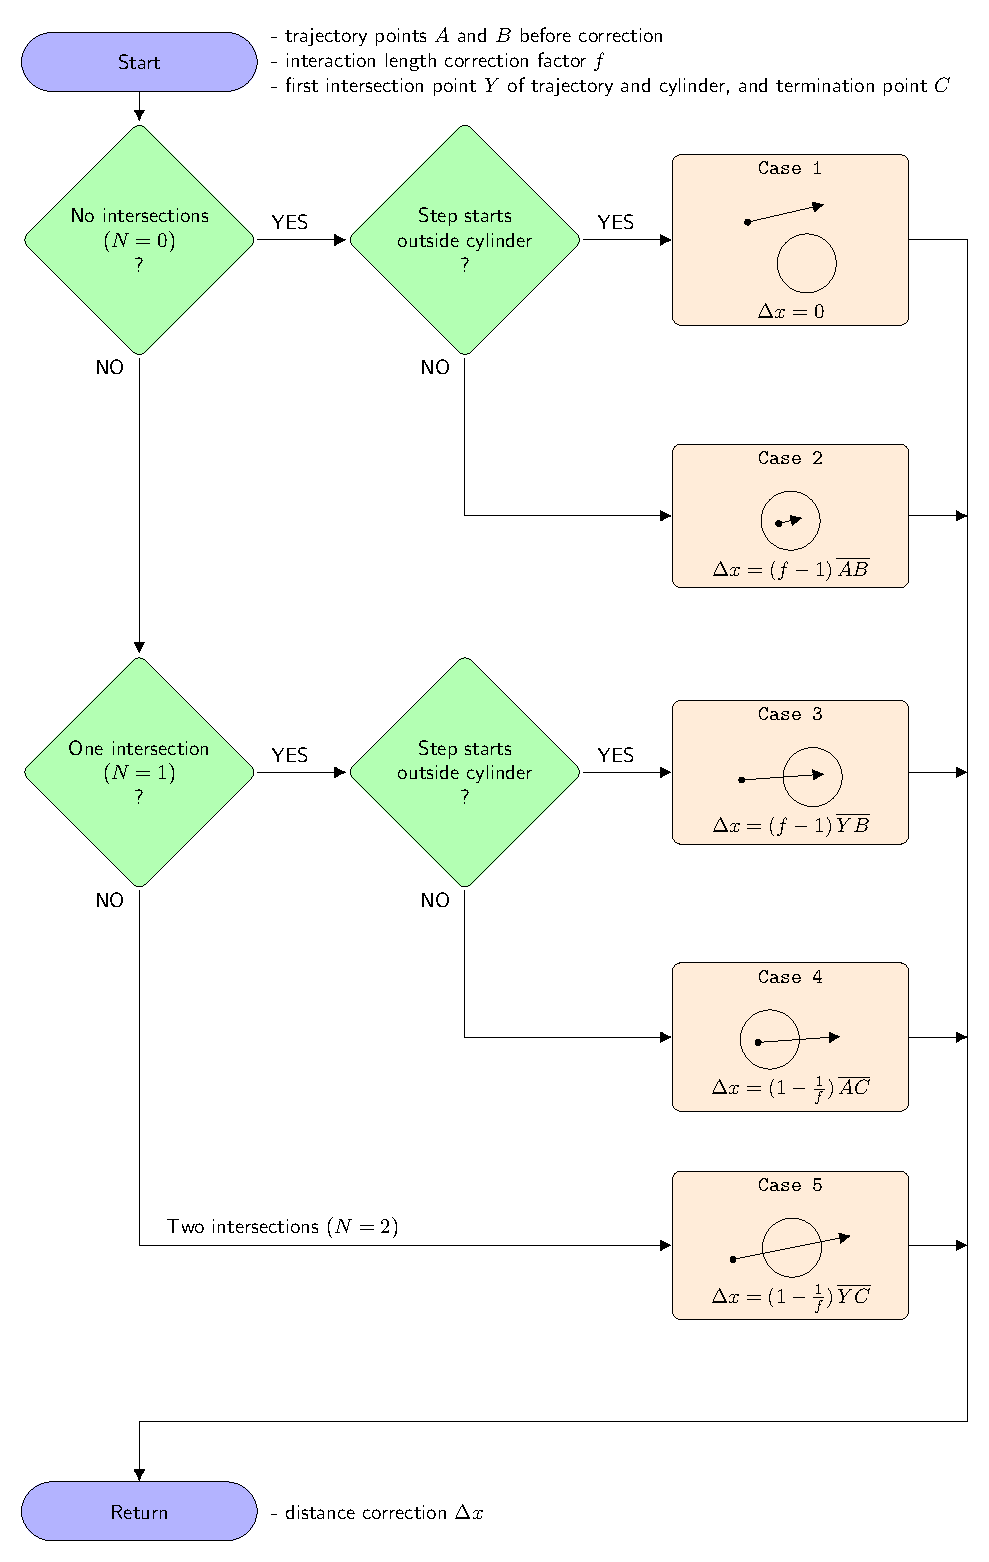
\includegraphics[height=\textheight]{img/algorithm-hole-ice-correction-2017-case-ordered}
  \caption{Flow chart for calculating the hole-ice correction for the geometric distance to the next interaction point.}
  \label{fig:Eeshi4Oh}
\end{figure}

\paragraph{Pros and Cons}

As this first hole-ice algorithm only adds subsequent corrections for
the standard-\clsim algorithm, it leaves the standard-\clsim code, which
is already well tested, almost untouched. The additions of the hole-ice
algorithm interface with the \clsim algorithm only through a small
surface area, corresponding to a small number of variables passed from
one algorithm to the other. This allows to test the hole-ice algorithm
with so-called \textit{unit tests} (section \ref{sec:unit_tests}) where
specific examples with fixed input variables are provided and tested
whether the algorithm produces the expected results for the example.

The hole-ice correction algorithm, however, has important limitations.
First, the current understanding of the hole ice suggests that the
interaction properties of the hole ice are independent of the properties
of the surrounding bulk ice (see section \ref{sec:hole_ice}). But with
this hole-ice correction algorithm, it is only possible to define the
interaction lengths of the hole ice relative to the interaction
properties of the surrounding bulk ice. While one could workaround this
problem locally by adjusting the correction factors \(f\) in relation to
the local properties of the bulk ice, large jumps over several layers of
ice with different properties would cause inevitable errors.

Secondly, the algorithm does work only correct in scenarios where the
photon crosses only one cylinder between two scattering points. In
scenarios where the photon crosses several cylinders, for example when
nested cylinders are used to model radially changing properties of the
hole ice, or when instantly-absorbing cylinders are used to model cables
within a hole-ice cylinder, this algorithm is not able to calculate the
corrections properly because it would interpret the interaction factors
\(f\) not only relative to the surrounding bulk ice but also relative to
the cylinders the photon has already crossed in this simulation step.

A different approach to adding propagation through hole-ice cylinders to
the standard-propagation algorithm is to treat hole-ice cylinders the
same way as other media such as ice layers rather than accounting for
the hole-ice effects using subsequent corrections. This second approach
gets rid of the above shortcomings, but at the cost that the
standard-\clsim algorithm that handles the propagation through different
media needs to be re-written. This second approach is described in the
following section.

  \subsection{Algorithm B: Hole-Ice Propagation by Generalizing the Previous Medium-Propagation Algorithm}
\label{sec:algorithm_b}

A second approach to adding propagation through hole-ice cylinders to
the standard propagation algorithm (section
\ref{sec:standardphotonpropagationalgorithm}) implemented in \clsim is
to rewrite the part of the standard algorithm that propagates the photon
through different media, aiming to make this algorithm more generic and
support hole-ice cylinders at the same level as other structures such as
ice layers.

\sourcepar{The source code of the implementation of this second approach can be found in appendix \ref{sec:algorithm_b_source}, in the folder \texttt{algorithm\_b} on the CD-ROM, as well as in the code repository at \url{https://github.com/fiedl/clsim/tree/sf/hole-ice-2018/resources/kernels/lib}.}

In order to propagate a photon through different media, the standard
propagation algorithm converts the randomized number of interaction
lengths \(N\) into a geometrical distance
\(X:=\sum_i n_i\,\lambda_i,\ N = \sum_i n_i\) (equation
\ref{eq:convertbudgettodistance} on page
\pageref{eq:convertbudgettodistance}) based on the interaction lengths
\(\lambda_i\) of the different media. In its current implementation in
\clsim, this conversion is hard-coded in a way that does support medium
changes in the form of tilted ice layers but does not support other
shapes such as cylinders of hole
ice.\footnote{A comparison of the flow charts of standard \clsim's media-propagation algorithm and the new media-propagation algorithm is given in appendix \ref{sec:flow_charts}.}
In the approach described in this section, the medium-propagation
algorithm is re-implemented in a way that does support cylinder-shaped
media.

\paragraph{Task}

The task of this new \textbf{medium-propagation algorithm} is to
determine in each simulation step, which media, including ice layers as
well as hole-ice cylinders, are on the photon's path along its current
direction and to convert the randomized scattering and absorption length
budgets to geometrical distances according to the interaction lengths of
the different media.

\paragraph{Context}

The new medium-propagation algorithm is inserted into the
\clsim propagation algorithm's simulation step right after \clsim has
randomized the number of scattering lengths to the next scattering
point, replacing \clsim's original medium-propagation algorithm. After
the medium-propagation algorithm follows the check whether the photon
hits an optical module on the way from the current scattering point
\(A\) to the next scattering point \(B\).

The medium-propagation algorithm takes the following input parameters:
Current photon position at point \(A\), photon direction after
scattering at point \(A\), a list of the hole-ice cylinders with their
coordinates, radii, scattering lengths and absorption lengths, a list of
ice layers with their coordinates, scattering lengths and absorption
lengths, the randomized number of scattering lengths to the next
scattering point, the remaining number of absorption lengths to the
absorption point, and the remaining geometric distance to absorption. As
output parameters, the medium-propagation algorithm returns the updated
number of remaining absorption lengths to the absorption point, the
geometric distance to the next scattering point, and the updated
remaining geometric distance to absorption.

\paragraph{Procedure}

The new algorithm works with a generic list of media. For each medium,
the algorithm stores the scattering length, the absorption length, and
the distance along the photon's direction from the current photon
position to the medium's border. This way, the algorithm knows in which
distance from the current position which medium properties take effect.
Due to this generic structure, homogeneous media with all kinds of
shapes could be added to this list. In this first implementation, the
algorithm adds un-tilted ice layers and cylinders, which model hole ice
and cables. Tilted ice layers as well as absorption anisotropy are not
re-implemented in this first implementation, but may be added
later.\footnote{At the time of writing, ice tilt and absorption anisotropy are not re-implemented, yet. To check the current state of this issue, see \url{https://github.com/fiedl/hole-ice-study/issues/48}.}
After adding ice layers and hole-ice cylinders to the media list, the
algorithm sorts the list by ascending distance from the current photon
position in order to have the list in the proper order for the following
calculations. Finally, the algorithm loops over the media list and
calculates the geometrical distances to the next scattering point and to
the absorption point just like the previous media-propagation algorithm
has done for ice layers only.

\paragraph{Media Loop}

In the loop over the different media along the photon's direction, the
algorithm calculates the contribution of the media to the geometrical
distances to the next scattering point and to the absorption point. The
flow chart of the whole media loop is shown in figure
\ref{fig:nimuriX4}. The flow chart for the calculation of one medium's
contribution is shown separately in figure \ref{fig:eewoo3Be}.

\begin{figure}[p]
  \resizebox{\textwidth}{!}{%
    \begin{tikzpicture}
  [
    %scale=1,
    node distance = 1.8cm,
    every node/.style = {fill=white, font=\sffamily},
    align = center
  ]

  % Nodes
  \newcommand\process[3]{\node(#1)[process, #3]{#2}}
  \newcommand\decision[3]{\node(#1)[decision, #3]{#2}}
  \node(start)[start]{Start};
  \decision{boundaryleft}{Medium\\boundary left\\?}{below = 2cm of start};

  \process{next}{Take next medium boundary}{right = 4cm of boundaryleft};
  \process{scadistance}{Calculate contribution of this medium\\up to the next medium boundary\\to the geometrical distance to the\\next \textbf{scattering} point}{below of = next};
  \process{absdistance}{Calculate contribution of this medium\\up to the next medium boundary\\to the geometrical distance to \textbf{absorption}}{below = 5mm of scadistance};

  \process{spendrestsca}{Calculate contribution of the last medium\\to the geometrical distance to the next scattering point}{below = 5cm of boundaryleft};
  \process{spendrestabs}{Calculate contribution of the last medium\\to the geometrical distance to absorption}{below of = spendrestsca};

  \decision{ifabsorbed}{Distance to\\absorption reached\\?}{below = 5mm of spendrestabs};
  \process{propagateonlytoabs}{Only propagate to the absorption point}{right = 2.5cm of ifabsorbed};

  \node(return)[stop, below = 2cm of ifabsorbed]{Return};

  % % Comments
  \newcommand\comment[2]{\node ()[substeps, right = 1mm of #1]{#2}}
  \comment{start}{
    \substep number of scattering lengths left to next scattering point\\
    \substep number of absorption lengths left to absorption\\
    \substep list of media. Each: distance to medium boundary, local scattering lenght, local absorption length
  };
  \comment{return}{
    \substep geometrical distance to next scattering point\\
    \substep geometrical distance to absorption
  };

  % Curly braces
  \makeatletter
    \@ifundefined{r@fig:eewoo3Be}{}{
      \draw [decorate, decoration={brace,amplitude=10pt,raise=4pt}, yshift=0pt]
        (absdistance.west) -- +(0,2.5) node [midway,xshift=-1.8cm] {See figure \ref{fig:eewoo3Be}};
    }
  \makeatother

  % Arrows
  \newcommand\connect[2]{\draw[->](#1)--(#2)}
  \connect{start}{boundaryleft};
  \connect{boundaryleft}{next};
  \connect{next}{scadistance};
  \connect{scadistance}{absdistance};
  \draw [->] (absdistance) |- +(5,-1.5) |- (0,-1.5);

  \connect{boundaryleft}{spendrestsca};

  \connect{spendrestsca}{spendrestabs};
  \connect{spendrestabs}{ifabsorbed};
  \connect{ifabsorbed}{propagateonlytoabs};
  \draw [->] (propagateonlytoabs) |- (0,-20.0);

  \connect{ifabsorbed}{return};

  % YES/NO labels
  \node () [right = 1mm of boundaryleft, yshift = 3mm] {YES};
  \node () [below = -1mm of boundaryleft, xshift = -5mm] {NO};

  \node () [right = 1mm of ifabsorbed, yshift = 3mm] {YES};
  \node () [below = -1mm of ifabsorbed, xshift = -5mm] {NO};

\end{tikzpicture}

  }
  \vspace*{5mm}
  \caption{Flow chart of the part of the new media-propagation algorithm that loops over list of media and calculates geometrical distances to the next scattering point and to the absorption point.}
  \label{fig:nimuriX4}
\end{figure}

\begin{figure}[htbp]
  \image{algorithm-media-loop-2018-calculation}
  \caption{Flow chart of the part of the new media-propagation algorithm that calculates the contribution of one specific medium to the geometrical distances to next scattering point and to the absorption point.}
  \label{fig:eewoo3Be}
\end{figure}

\paragraph{Contribution of the Last Medium}

As shown in figure \ref{fig:nimuriX4}, the last medium is handled
separately as the contribution of the last medium is not determined by
the size of the medium but by the amount of scattering and absorption
budget left. The contributions of the first \((m-1)\) media to the
geometrical distance sum up to \(\sum_{i=1}^{m-1} x_i\) where each
contribution \(x_i := n_i\,\lambda_i\) determines how much of the budget
\(N:=\sum_{i=1}^m n_i\) is spent. After the first \((m-1)\) media have
been crossed, \(n_m := N - \sum_{i=1}^{m-1} n_i\) of the budget is left
for the last medium. Thus, the photon travels a distance of
\(x_m := n_m\,\lambda_m\) in the last medium where it reaches the
interaction point.

\paragraph{Absorption Before Reaching the Scattering Point}

When calculating the distance to the next scattering point based on the
scattering length budget, if the photon's absorption length budget is
spent before reaching the next scattering point, or equivalently, if the
distance from the current scattering point \(A\) to the absorption point
is shorter than the distance from \(A\) to the next scattering point,
then the next trajectory point \(B\) is set to be the absorption point
as shown in figure \ref{fig:nimuriX4}. The final trajectory point of the
photon is its point of absorption.

\paragraph{Scattering Before Reaching the Absorption Point}

When calculating the contribution of a medium to the remaining distance
to the absorption point as shown in the lower half of figure
\ref{fig:eewoo3Be}, the algorithm needs to know what distance \(\gamma\)
within that medium contributes to spending the absorption length budget.
If the photon does not scatter within this medium, the distance
\(\gamma\) is just the distance from one medium border to the next
medium border along the photon
direction.\footnote{This corresponds to the termination point being set to the second intersection point, $C = X$, in Case 4 and Case 5 of the hole-ice-correction algorithm described in section \ref{sec:algorithm_a}.}
If the photon does scatter within this medium, the distance \(\gamma\)
is set to the distance to the scattering
point\footnote{This corresponds to the termination point being set to the point of the other interaction in Case 4 and Case 5 of the hole-ice-correction algorithm described in section \ref{sec:algorithm_a}.}
as shown in the upper half of figure \ref{fig:eewoo3Be}.

\paragraph{Order and Precedence of Cylinders}

\begin{figure}[htbp]
  \subcaptionbox{In a case where the inner cylinder is smaller, intuition suggests that the inner cylinder represents a special area within a more general area and should take precedence for a photon located within both cylinders.}{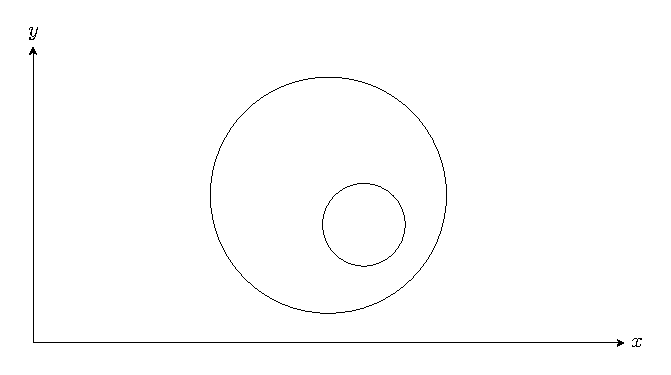
\includegraphics[width=0.48\textwidth]{img/cylinder-order-kuZ8deek}}\hfill
  \subcaptionbox{If both overlapping cylinders have the same size, the choice which properties should be applied to a photon at a position within the overlap of both cylinders, is arbitrary. }{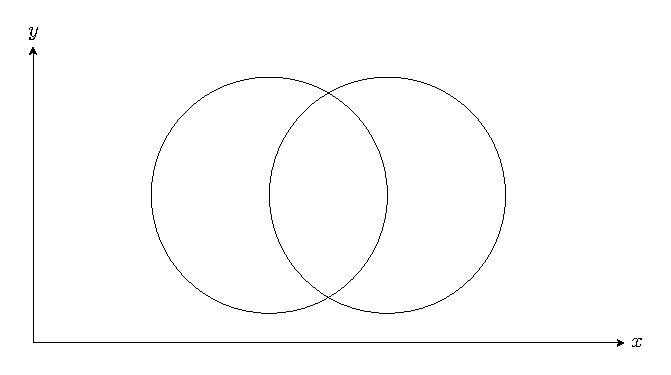
\includegraphics[width=0.48\textwidth]{img/cylinder-order-Yeifohm3}}
  \caption{Two-dimensional projection of nested or overlapping hole-ice cylinders with different ice properties. If a photon is at a position within the overlap of both cylinders, which ice properties should be applied for the propagation? The algorithm defines that the cylinder added last takes precedence.}
  \label{fig:kuZ8deek}
\end{figure}

When nesting or overlapping cylinders as shown in figure
\ref{fig:kuZ8deek}, the algorithm needs to determine which ice
properties to apply for a photon at a position within both cylinders. In
the left part (a) of the figure, the intuition might be: The smaller
cylinder models a special area within the more general outer cylinder
and, therefore, should take precedence. In the right part (b) of the
figure, however, both cylinders have the same size. Here it is unclear
which ice properties to apply for a position within the cylinders'
overlap. To make this situation unambiguous, the algorithm defines that
the media added to the list later take precedence over media added
earlier. Therefore, when modeling nested cylinders, the algorithm
requires to add the larger cylinder before adding the smaller cylinder
to the definition list.

\paragraph{Pros and Cons}

This second approach allows to define cylinder-shaped volumes with
absolute scattering and absorption lengths, which meets the requirements
of the current understanding of the hole-ice phenomenon. Simulation
steps over large \(z\)-distances that cross hole-ice cylinders are
handled well by this algorithm in contrast to the previously described
hole-ice-correction algorithm (section \ref{sec:algorithm_a}).
Additionally, this algorithm supports nested or overlapping cylinders,
which can be utilized to model bubble column together with the
drill-hole column as well as the string's cable. Ice tilt and absorption
anisotropy have not been ported to this algorithm, yet, but can be added
later
on.\footnote{See: \url{https://github.com/fiedl/hole-ice-study/issues/48}.}

The down side to this approach is that an important part of
standard-\clsim's media-propagation algorithm needed to be
re-implemented, requiring evidence that the new algorithm is still doing
what is expected. In order to provide this evidence, section
\ref{sec:unit_tests_and_cross_checks} describes a series of cross checks
to make sure the new algorithm results in the expected scattering and
absorption behavior. Also, standard-\clsim's medium-propagation has been
ported to the new interfaces as drop-in replacement for the new
medium-propagation algorithm, such that one can switch between both
algorithms without a code
rollback.\footnote{A guide on how to switch the medium-propagation algorithm is presented in appendix \ref{sec:how_to_switch_media_propagation}.}

\begin{table}
  \begin{tabelle}{l|L|L}
    & \textbf{Algorithm (a)} & \textbf{Algorithm (b)} \\
    \hline
    Approach
      & Leave \clsim medium propagation as it is and add \textbf{hole-ice effects as correction} afterwards
      & Unify \clsim medium propagation through layers and hole ice: Treat them as \textbf{generic medium changes} \\
    Hole-ice properties
      & defined relative to bulk-ice properties
      & defined absolute \\
    Pros
      &
        \begin{itemize}
          \item[+] Small surface area of hole-ice code, well testable through unit tests
          \item[+] Standard \clsim almost untouched
        \end{itemize}
      &
        \begin{itemize}
          \item[+] Supports nested cylinders and cables
        \end{itemize}
      \\
    Cons
      &
        \begin{itemize}
          \item[--] Current understanding of hole-ice suggests defining hole-ice properties absolute rather than relative
        \end{itemize}
      &
        \begin{itemize}
          \item[--] Needed rewrite of \clsim's medium-propagation code
          \item[--] Ice tilt and ice anisotropy not re-implemented, yet
        \end{itemize}
  \end{tabelle}
  \caption{Comparison of the hole-ice-correction algorithm (a) presented in section \ref{sec:algorithm_a} and the new generic medium-propagation algorithm (b) presented in section \ref{sec:algorithm_b}.}
\end{table}

A comparison to other methods to account for the hole-ice effect is
presented in section \ref{sec:comparison_methods}.

  \subsection{Technical Issues and Optimizations}
\label{sec:technical_issues_and_optimizations}

Running a simulation with millions of photons propagating and
scattering, has to meet certain performance requirements that make sure
that the simulations of interest can be run in a reasonable time on
current hardware. On the other hand, current graphics processing units
(GPUs) afford the opportunity to utilize parallelization capabilities.
Both impose technical challenges. To deal with the necessary complexity
and, in particular, to make sure that a complex algorithm does what it
is supposed to do, unit tests and cross checks are used as will be
described in the next section \ref{sec:unit_tests_and_cross_checks}.
This section focuses on dealing with computational limits, introducing
the techniques of GPU parallelization, cluster parallelization,
thinning, and performance optimizations.

\paragraph{Simulation-Step Parallelization}

Each simulation step consists of only a few operations: Scattering the
photon, checking for absorption, checking for collision with a detector
module, and propagating the photon to the next scattering position (see
\ref{sec:standard_photon_propagation_algorithm}). This small set of
operations can be parallelized, performing the same calculations and
operations simultaneously for several thousands of simulation steps,
each with different values such as coordinates and directions, on
graphics processing units, which are designed for exactly this kind of
work. Figure \ref{fig:Id3ioyie} illustrates this parallelization of
simulation steps.

\begin{figure}[htbp]
  %\image{dima-parallel-photons-Id3ioyie}
  \hspace{1.5cm}
  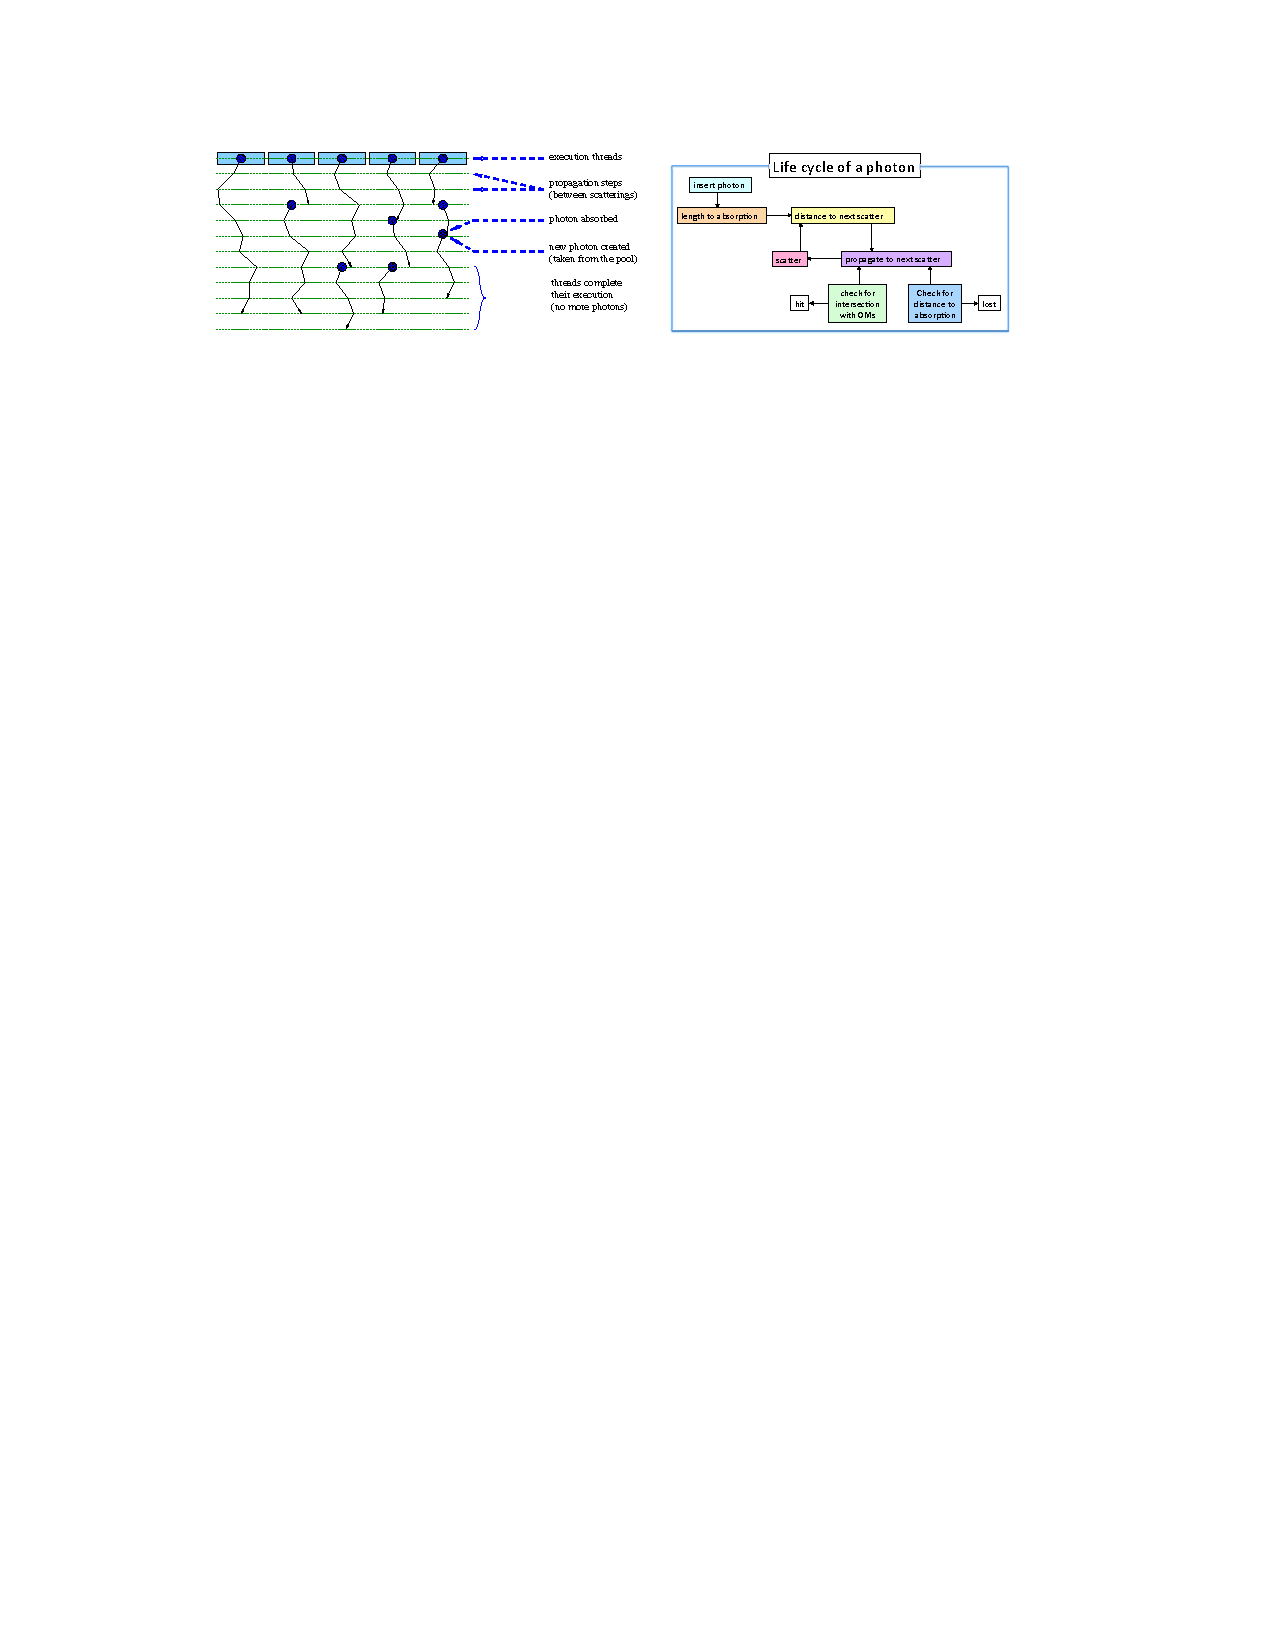
\includegraphics[width=0.7\textwidth, trim={7.7cm 0 0 0}, clip]{img/dima-parallel-photons-Id3ioyie}
  \newline\hspace*{1.5cm}
  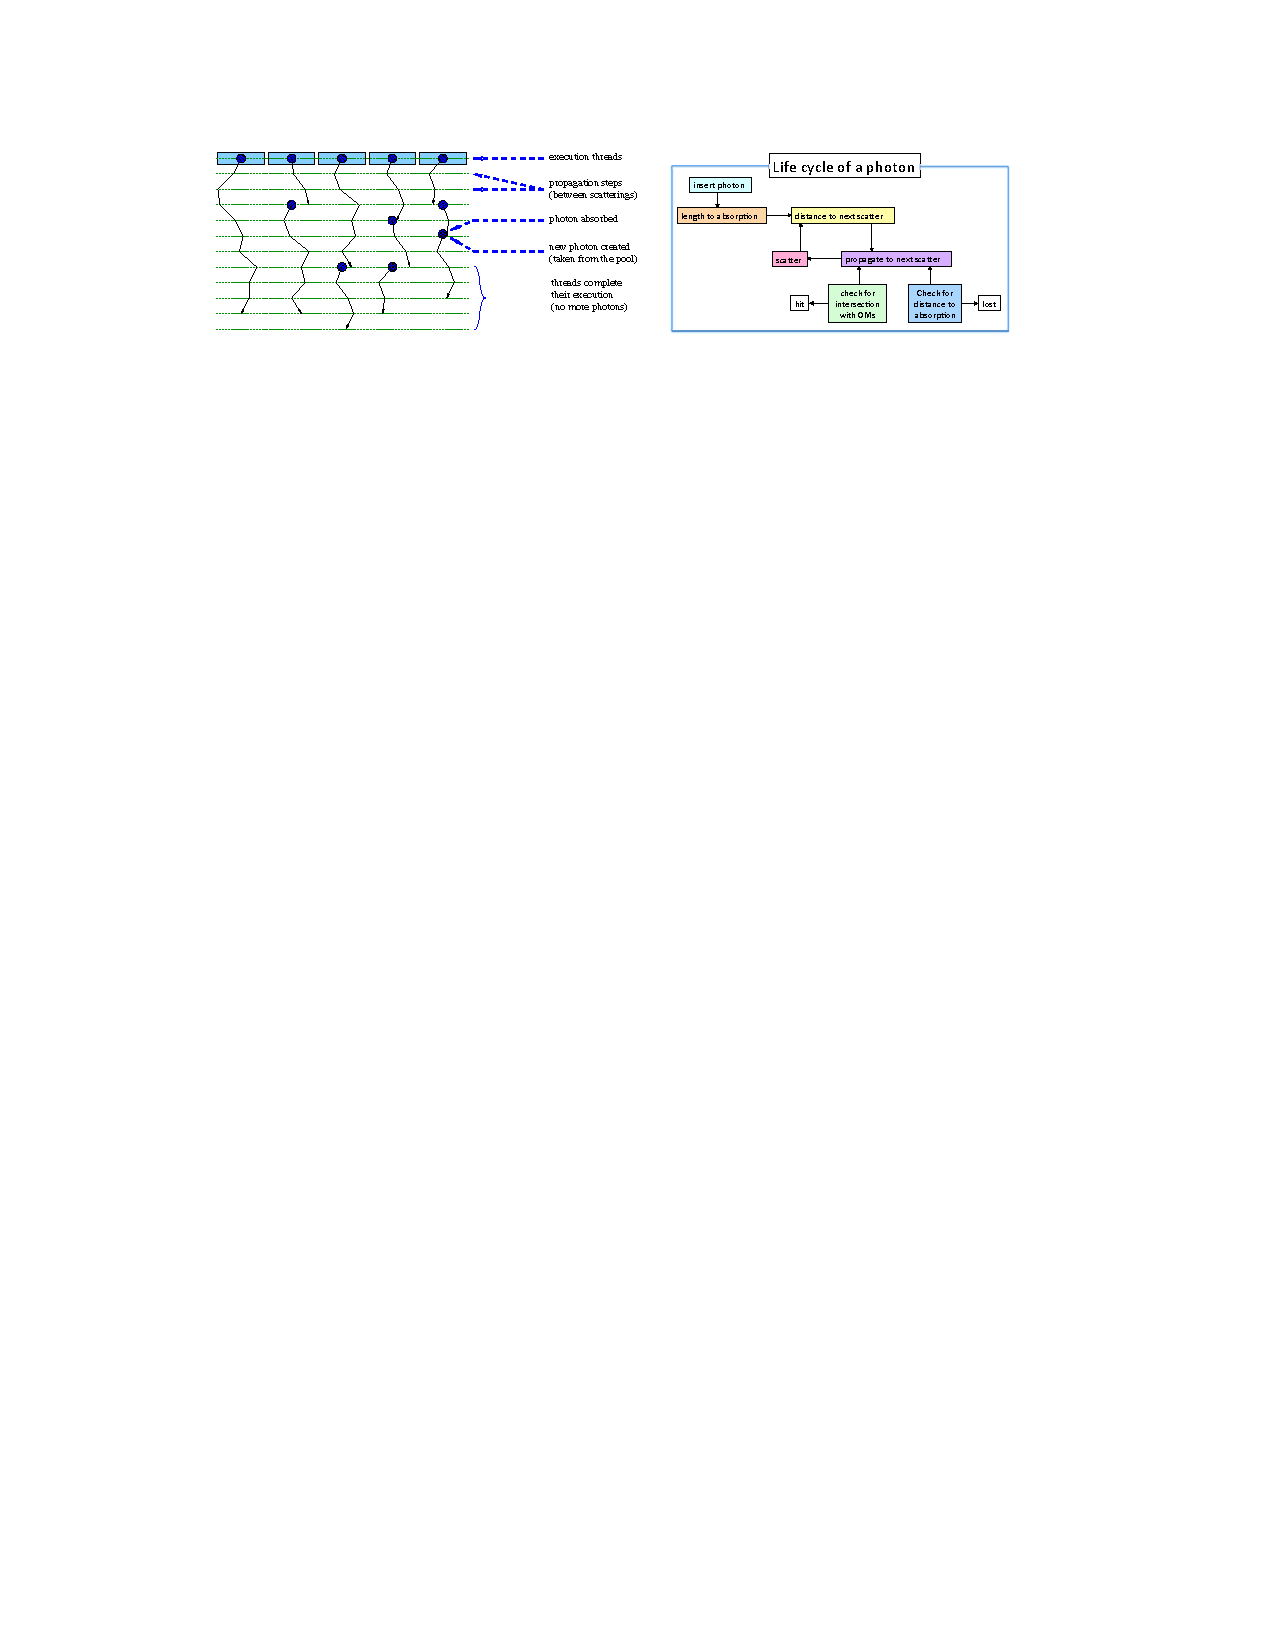
\includegraphics[width=0.9\textwidth, trim={0 0 6.2cm 0}, clip]{img/dima-parallel-photons-Id3ioyie}
  \caption{Parallelization of simulation steps: Tracking of photons entails the computationally identical steps: Propagation to the next scatter, calculation of the new direction after scatter, and evaluation of intersection points of the photon track segment with the detector array. These same steps are computed simultaneously for thousands of photons. (Image and caption taken from \cite{ppcpaper}, figure 1.)}
  \label{fig:Id3ioyie}
\end{figure}

This parallelization leads to a performance improvement by factors of
150 and more when running the propagation simulation on a single GPU
compared to running the same simulation on a single CPU core
\cite{ppcpaper}. Standard \clsim as well as the hole-ice extended
\clsim can be run on CPUs, GPUs, or both using \noun{OpenCL} as
abstraction layer. In practice, simulating 1000 photons for
visualization purposes and recording their paths, which requires a lot
of memory, works best on a CPU. Simulating millions of photons, but only
recording their final position, where the photon is absorbed within the
ice or has it an optical module, works best on GPUs.

\paragraph{Cluster Parallelization}
\label{sec:cluster_parallelization}

A different technique, which adds another layer of parallelization on
top of the simulation-step parallelization, is to run the same
simulation on a cluster of machines, each equipped with one ore several
GPUs. Each machine runs the same simulation, but with different
parameters, such as different radii and scattering lengths of the
hole-ice cylinders. This study uses this technique for parameter scans
(sections \ref{sec:parameter_scan} and \ref{sec:flasher}) where the same
simulation is performed for different parameter sets in order to find a
specific parameter set which best fits some kind of external
requirement.

\paragraph{Issues Concerning Graphics Processing Units}

Running and developing a simulation software for graphics processing
units poses challenges specific to this architecture. A list of
technical issues to watch out for in follow-up studies is provided in
appendix \ref{sec:gpu_technical_issues}.

\paragraph{Parallel-Programming Optimizations}

Applying parallel-programming optimization techniques listed in section
\ref{sec:parallel_computing} may help to improve the performance of the
algorithm that runs on the graphics processing units.

When optimizing code, \noun{Ahmdal's Law} gives the theoretical limit on
how much a process can be sped up by optimizing one of its components.
\cite{raytracingtips}

\[ s_\text{total} = \frac{1}{(1 - p) + \sfrac{p}{s_\text{comp}}}, \ \ \ s = \frac{t_\text{before}}{t_\text{after}}, \ \ \
\lim_{s_\text{comp}\rightarrow\infty} s_\text{total} = \frac{1}{1-p} \]

Here, \(s_\text{total}\) is the resulting speedup of the whole process,
which is defined as the fraction of the time the process takes before
the optimization and the time the same process takes after the
optimization has been applied. \(p\) is the portion of execution time
that the component requires before optimizing. \(s_\text{comp}\) is the
speedup the the component that is optimized achieved by the
optimization. Even in the limit that the component that is optimized
takes zero time after applying the optimization,
\(s_\text{comp}\rightarrow\infty\), the speedup of the whole process is
limited. Also, \authorname{House} and \authorname{Wyman}
\cite{raytracingtips} recommend to first write working code, and then
optimize in a second step.

One key concept to efficient parallel programming is to avoid
executional threads being idle, waiting for other threads to finish
before resuming. One application of this concept in the hole-ice
algorithm is to \textbf{filter hole-ice cylinders by range} in a
\textbf{separate loop}. The algorithm needs to check in each simulation
step, which hole-ice cylinders are in range of the photon and therefore
should be considered when calculating the propagation through the hole
ice. Without this optimization, the cylinders are processed one by one
in each simulation step. While, in each iteration of the cylinder loop,
all photons in range of one specific cylinder are propagated through
that cylinder, all other photons not in range of the cylinder, wait idly
and thereby waste computation time. This is illustrated in figure
\ref{fig:ceiV8Yai} (a).

Even though the optimization adds time for the additional loop where the
indices of the cylinders in range are saved into a local array, the main
loop where the propagation through each cylinder is handled is much
faster now, because it does not need to iterate over all cylinders in
the detector but only over the cylinders in range of the photon and
improves parallelization as illustrated in figure \ref{fig:ceiV8Yai}
(b).

\docpar{The implementation of this optimization is documented in \issue{30}.}

\begin{figure}[htbp]
  \subcaptionbox{Checking if a cylinder is in range in the same loop as propagating through that cylinder. The cylinders are processed successively. Lots of photons are idle.}{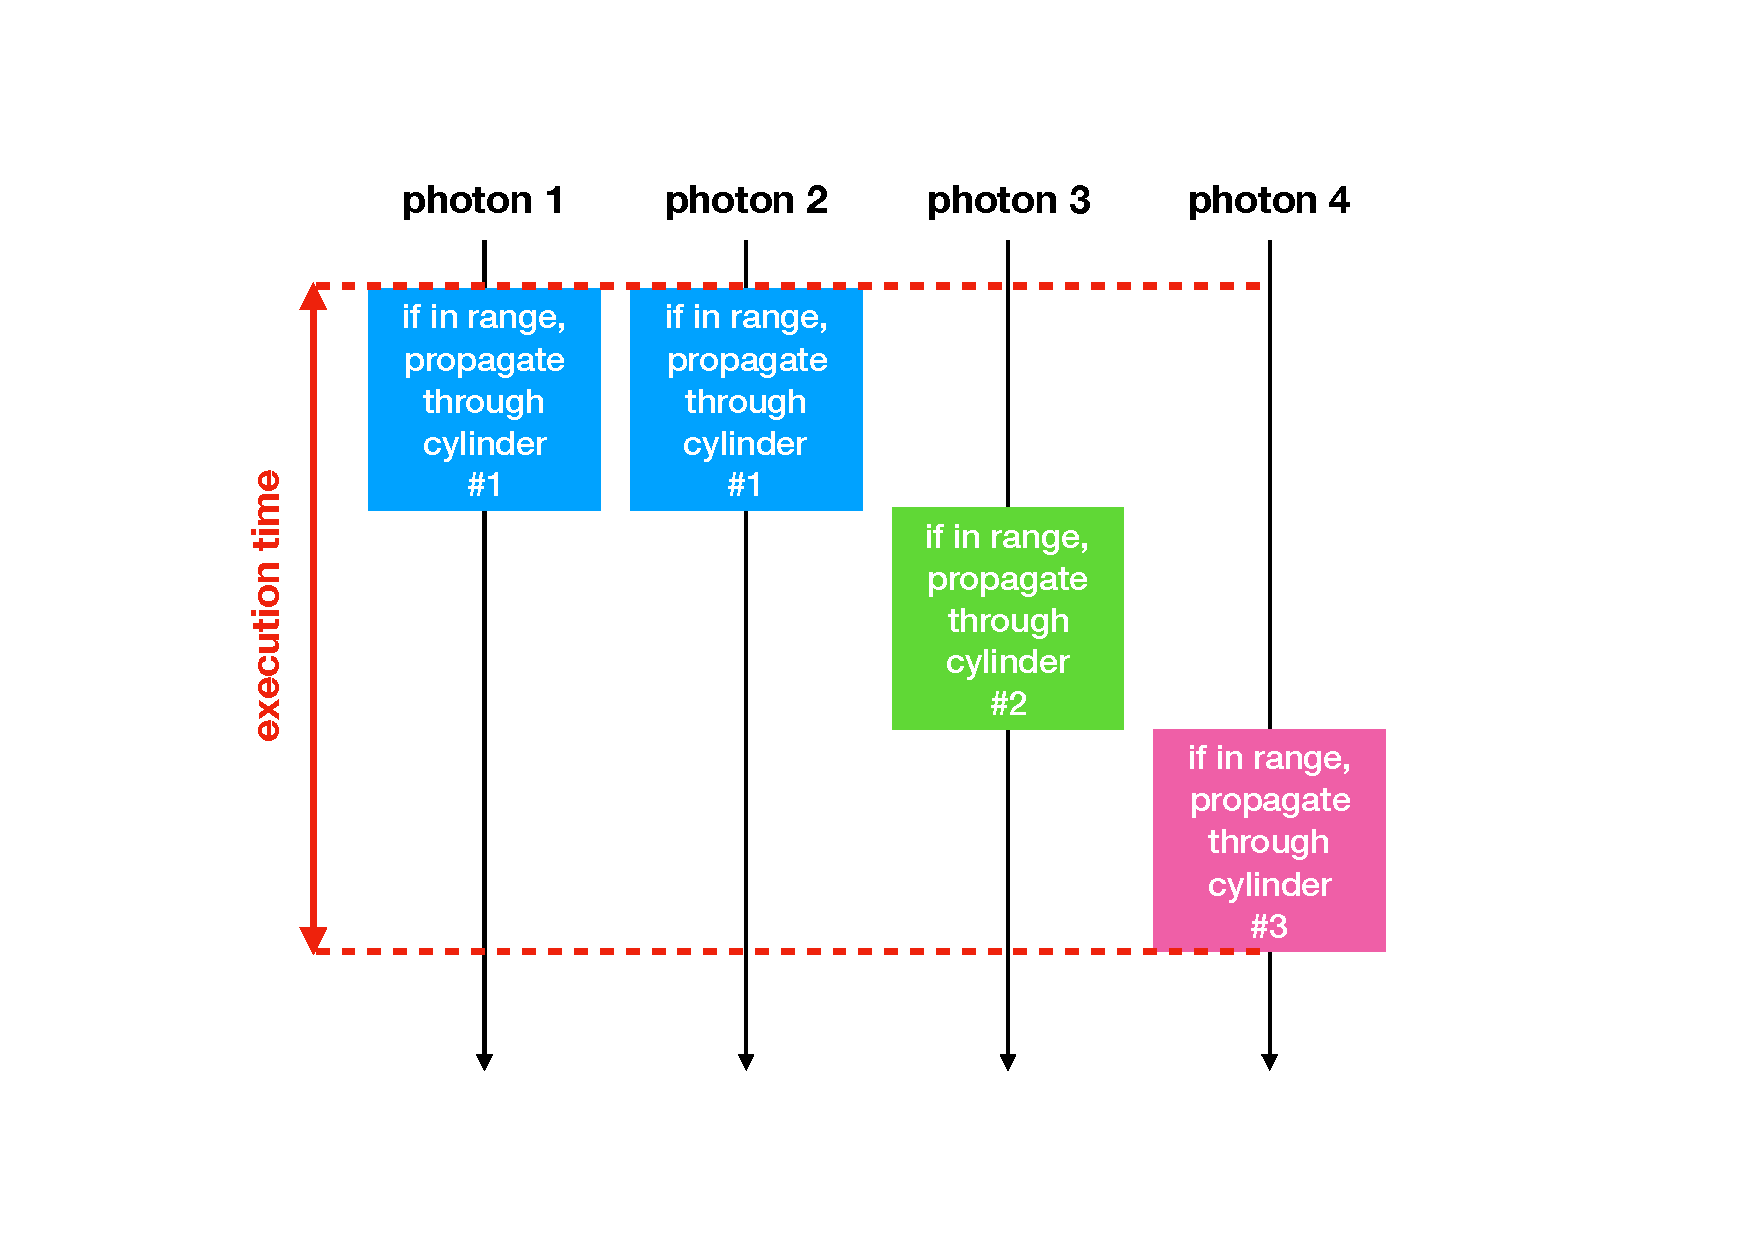
\includegraphics[width=0.48\textwidth, clip, trim = {4cm 2cm 6cm 2cm}]{img/cylinder-sort-ceiV8Yai}}\hfill
  \subcaptionbox{Checking if a cylinder is in range in a separate loop. The main loop where the photons are propagated through the cylinders does not loop over all cylinders but only over cylinders marked as in range for each photon respectively. }{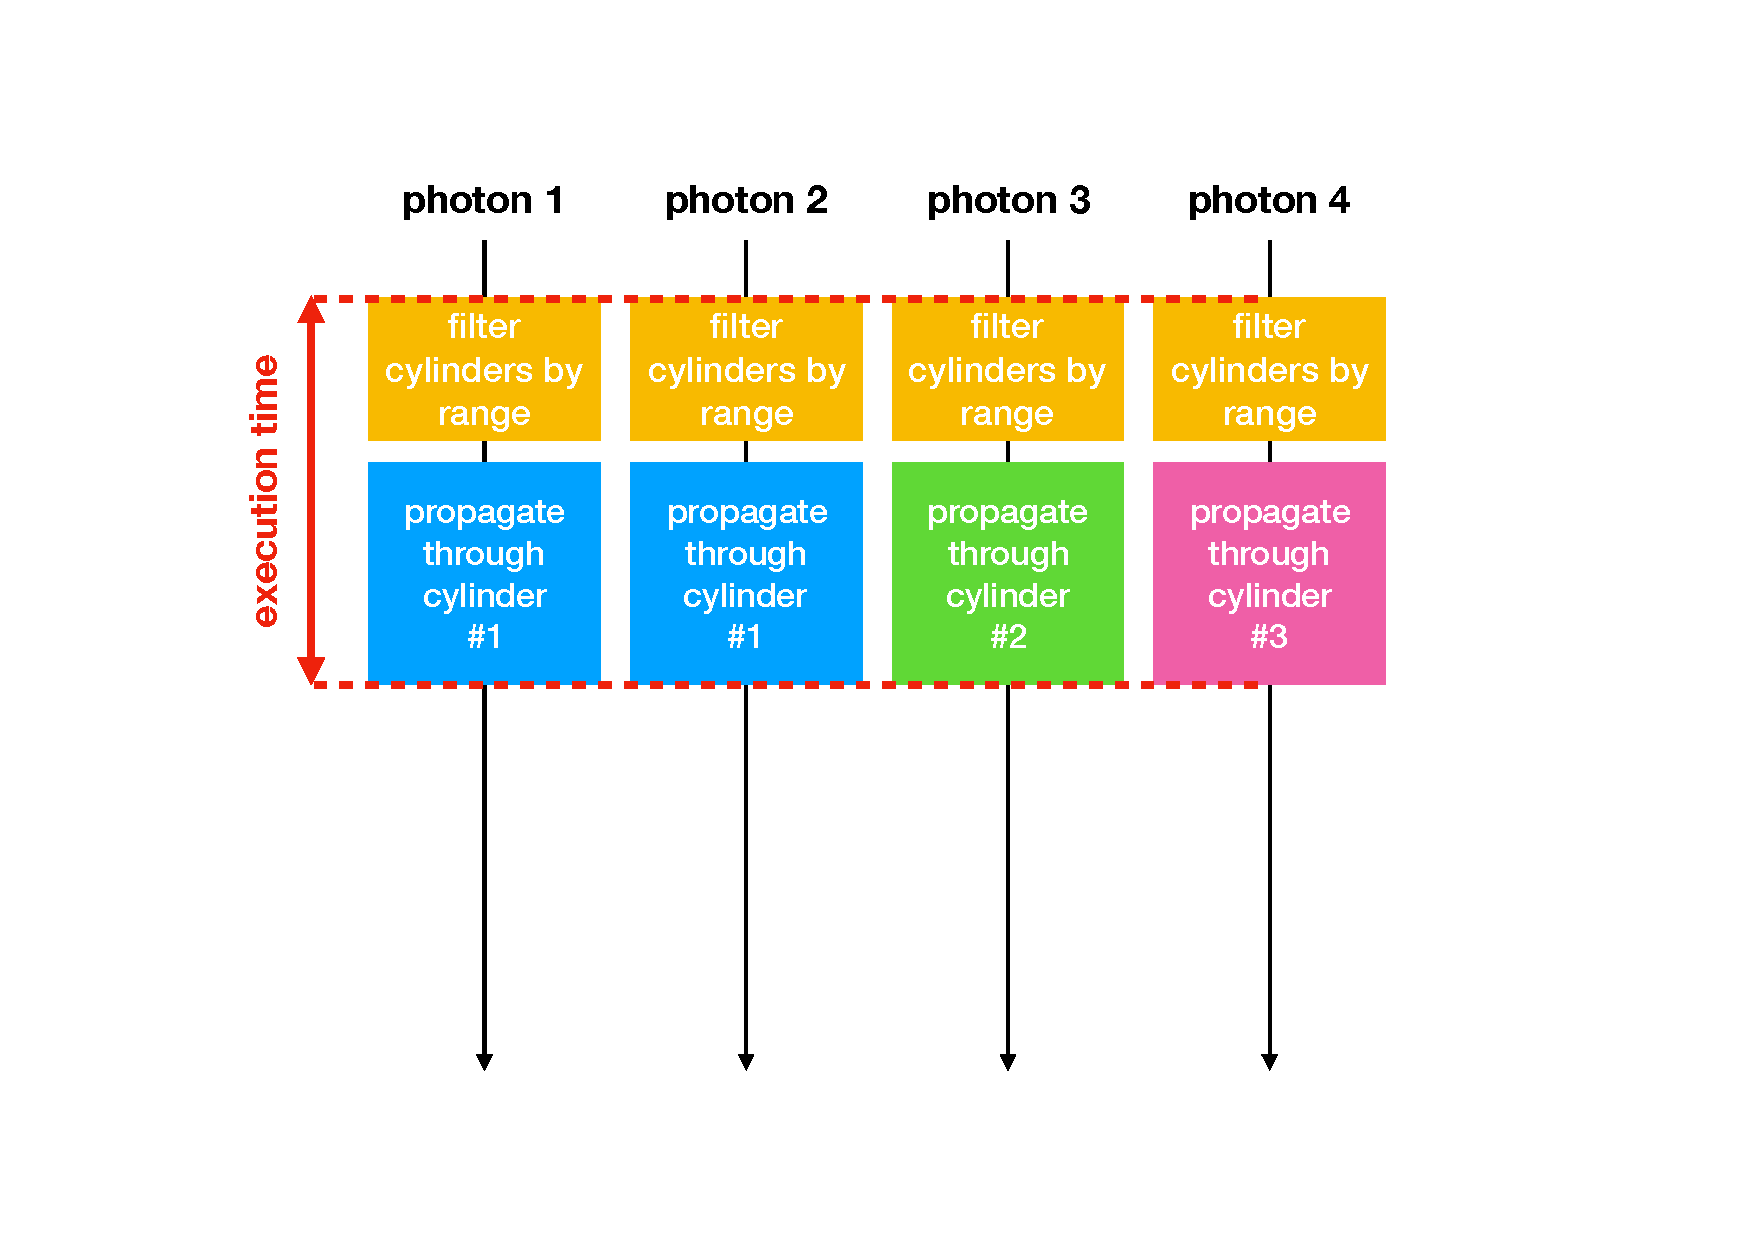
\includegraphics[width=0.48\textwidth, clip, trim = {4cm 2cm 6cm 2cm}]{img/cylinder-sort-compact-ceiV8Yai}}
  \caption{Processing the propagation of photons through hole-ice cylinders in parallel. While filtering cylinders by range separately adds additional executional time, it improves parallelization and thereby saves execution time overall.}
  \label{fig:ceiV8Yai}
\end{figure}

Another optimization used in the hole-ice algorithm is to
\textbf{order mathematical cases by their frequency of application}. In
a case-by-case analysis, each executional thread skips the additional
case checks when its case is determined. If the checks for common cases
are handled first, there is a good chance that all of the parallel
threads fall into common cases such that the checks for the rare cases
can be skipped for the whole thread block. This technique is used in the
implementation of the geometric cases for both the hole-ice-correction
algorithm (\ref{sec:algorithm_a}) and the new media-propagation
algorithm (\ref{sec:algorithm_b}).

\paragraph{GPU-Specific Optimizations}

In addition to the general principles of parallel programming (section
\ref{sec:parallel_computing}), \authorname{House} and \authorname{Wyman}
\cite{raytracingtips} list practical tips for optimizing GPU-ray-tracing
code. Most notably, passing data structures by reference rather than by
value proved to have significant performance impact because
\textbf{allocating memory on a GPU is expensive}. This also includes
simple structures like arrays of numbers, and even re-using the same
array for several calculations rather than re-defining it. This
technique has caused a performance improvement on GPUs by a factor of
six in this study.

\docpar{This optimization of re-using arrays is documented in \issue{70}.}

\textbf{Optimizing mathematical operations} on paper is an important
technique as each calculation operation that can be cut down on in a
procedure that saves time when executing the procedure many times. In
addition to simplifying equations mathematically, avoiding numerically
expensive operations such as square roots improves performance.

GPUs support 4-dimensional vectors as native data types as well as
native vector operations such as the dot product. Expressing equations
in terms of vectors rather than simplifying equations on the coordinate
level, resulted in improved performance and numerical accuracy.

\docpar{This optimization of using vector types rather than scalar types is documented in \issue{28}.}

\paragraph{Performance Profiling}

\authorname{Owens} recommends profiling tools like \noun{gprof},
\noun{VTune}, or \noun{VerySleepy} \cite{cudacourse}. But also basic
techniques like printing time differences between executional blocks can
help to isolate performance problems. Figure
\ref{fig:profiling-paz4Eig6} shows the execution time profile of the
simulation step of the new medium-propagation algorithm.

Note that printing a profiling result may be more expensive as the
computation that is to be profiled itself. In this study, printing the
time difference of the beginning and the end of a simulation step takes
five times as long as the simulation step itself.

\docpar{Profiling the simulation step is documented in \issue{69}.}

\begin{figure}[htbp]
  \image{profiling-paz4Eig6}
  \caption{Performance profile of the average simulation step in arbitrary units (GPU clock cycles). Each row of the chart represents a different algorithm. In the first row, which shows an early stage of the new medium-propagation algorithm, the initial memory allocation within each simulation step takes a lot of time, especially when comparing to standard \clsim (row 3). The second row shows the profile of the new medium-propagation algorithm after a memory issue has been fixed. Notable operations in each simulation step are the initial memory allocation for local variables, adding ice layers, adding hole-ice cylinders, sorting medium boundaries by distance to the photon and looping over the media to convert the interaction budget into geometrical distances.}
  \label{fig:profiling-paz4Eig6}
\end{figure}

\paragraph{Performance Optimizations for Production Use}

After implementing and debugging a new algorithm, a lot of debug outputs
and other development tools are no longer required when running
simulations. For those production simulations, the debug features can be
turned off by
\textbf{compiling the \icecube simulation framework for production} use
rather than for debugging. Thereby, simulations run significantly faster
as debug outputs often cost more time than the actual simulation itself.

Also, activating \textbf{kernel caching} on the production machines may
improve simulation performance. However, this should only be used when
always using the same propagation kernel, and should be avoided when
switching between kernel versions or turning kernel features on and off,
because the kernel cache will not be reliably reset automatically when
changing kernels.

\label{sec:thinning} Another way to save computational time when
performing simulations, especially large cluster scans, is to scale down
the number of photons using a \textbf{thinning factor}. A representative
fraction of the photons is propagated in the simulation, and then the
simulation results, for example the numbers of hits in each detector
module, are scaled up accordingly.

\docframe{
  \docparwithoutframe{How to switch between a debug build and a production build is documented in \issue{73}.}\medskip

  \docparwithoutframe{How to enable or disable kernel caching is documented in \issue{15}.}\medskip

  \docparwithoutframe{Using a thinning technique in flasher parameter scans is documented in \issue{59}.}
}

  \subsection{Unit Tests and Cross Checks}
\label{sec:unit_tests_and_cross_checks}

There are several techniques to ensure that the propagation algorithm
produces results that meet the expectations. First, \clsim itself
implements a number of tests that run in each simulation and check
computational quantities for consistency. \cite{clsimsource}

Secondly, one can define scenarios with known quantities for single
photons and check externally whether the algorithm produces the expected
results for those single photons. This is done with \textit{unit tests}
and is presented in section \ref{sec:unit_tests}.

Thirdly, checks for a sample of photons can be devised where all photons
should behave the same way, for example all photons should be absorbed
by a medium that is configured for instant absorption. This check is
presented in section \ref{sec:instant_absorption_tests}.

Finally, a sample of propagated photons can be examined regarding their
statistical properties, for example the sample's distributions of
quantities like arrival time and path length. These tests are presented
in sections \ref{sec:arrival_time} to \ref{sec:cross_check_71}.

\subsubsection{Unit Tests With Single
Photons}\label{unit-tests-with-single-photons}

\label{sec:unit_tests}

In order to verify that individual components (``units'') of the
implementation produce results as expected, unit tests were implemented
for the algorithm that calculates intersections as well as for the
hole-ice-correction algorithm.

\docframe{
  \sourceparwithoutframe{The unit tests for the intersection algorithm can be found in the folder \texttt{unit\_tests} on the CD-ROM and at \url{https://github.com/fiedl/clsim/blob/sf/hole-ice-2017/resources/kernels/lib/intersection/intersection_test.c}.}\medskip

  \sourceparwithoutframe{The unit tests for the hole-ice-correction algorithm can be found in the folder \texttt{unit\_tests} on the CD-ROM and at \url{https://github.com/fiedl/clsim/blob/sf/hole-ice-2017/resources/kernels/lib/hole_ice/hole_ice_test.c}.}
}

\paragraph{Task}

The task of unit tests is to test individual components of a software.
In this case, the tests execute separate functions of the new algorithms
with fixed input parameters and check whether the functions return the
expected results, which, in preparation of the test, have been obtained
by other means, either by a separate program, using a separate
programming language, a separate algorithm, or via calculations by hand.

In this study, unit tests define single photons that cross hole-ice
cylinders in a pre-defined way and check whether the intersection
algorithm determines the correct intersection points, whether the 2d-3d
projections are handled correctly, and whether the hole-ice-correction
algorithm determines the expected corrections for the geometric
distances according to the hole-ice parameters provided by the test
scenario. Extreme examples can be designed to produce simple results
that can be calculated by hand and verified by intuition. For example,
for hole-ice cylinders configured for instant absorption, the absorption
point is identical to the intersection point of the photon trajectory
and the cylinder. More complex examples require more involved
calculations by hand or using other software like \noun{Python} scripts
or computer algebra tools for calculating intersections.

\paragraph{Testing Framework}

This study uses the
\noun{gtest}\footnote{Google Test Framework, gtest, \url{https://github.com/google/googletest}}
testing framework. This framework has been chosen due to its good
documentation, wide adoption and slim architecture that made it possible
to use the framework to test individual components of the new source
code without interfering with the rest of the \icesim framework.

\docpar{The introductory documentation of \noun{gtest} can be found at \url{https://github.com/google/googletest/blob/master/googletest/docs/primer.md}.}

\paragraph{Limitations of Unit Tests}

Unit tests are most useful to ensure stability when adjusting,
refactoring or rewriting software components. Even after replacing a
large part of the source code, unit tests can make sure that the
software still produces the same results as before. Tests also allow for
so-called test-driven development where the expected results are
specified first, and then the software is built or changed iteratively
until it produces the expected results. This technique works best when
the components to be tested have small interfaces because the technique
requires the tests to provide all input parameters for the components to
be tested.

Unexpected issues may arise when unit tests are run on another
architecture as the production code. For example, the unit tests used in
this study were insensitive to certain driver issues and numerical
issues\footnote{See section \ref{sec:gpu_technical_issues}.} that did
only occur when running the software on the GPUs of the computing
cluster and did not occur when running the unit tests on the local CPU
of the development machine.

Unit tests are, by design, also insensitive to high-level problems. Each
individual component may produce the results expected from this
component while still issues may arise when components are not tied
together correctly, or because the expectations for an individual
component may be wrong, which becomes apparent only when adopting a
larger perspective rather than the focused perspective on individual
components.

To increase confidence in the new software, therefore, in addition to
unit testing, high-level cross checks need to be performed as described
in the following subsections.

\subsubsection{Instant-Absorption Tests}\label{instant-absorption-tests}

\label{sec:instant_absorption_tests}

A simple high-level test can be performed by starting several photons
towards a cylinder, which is configured for instant absorption. After
propagating the photons using the new media-propagation algorithm and
recording the path of each individual photon, one can verify the results
making sure than no photon position is recorded inside the
instant-absorption cylinder (figure \ref{fig:chiep7Is}). Additionally,
one can visualize the simulation using the \steamshovel event viewer to
verify that no photon enters the instant-absorption cylinder as shown in
figure \ref{fig:moo9Eiqu}.

\sourcepar{The implementation of this cross check can be found in \issue{67}, \issue{47}, and \issue{22}.}

\begin{figure}[htbp]
  \subcaptionbox{Distribution of the distance to the hole-ice center, evaluated for each scattering step.}{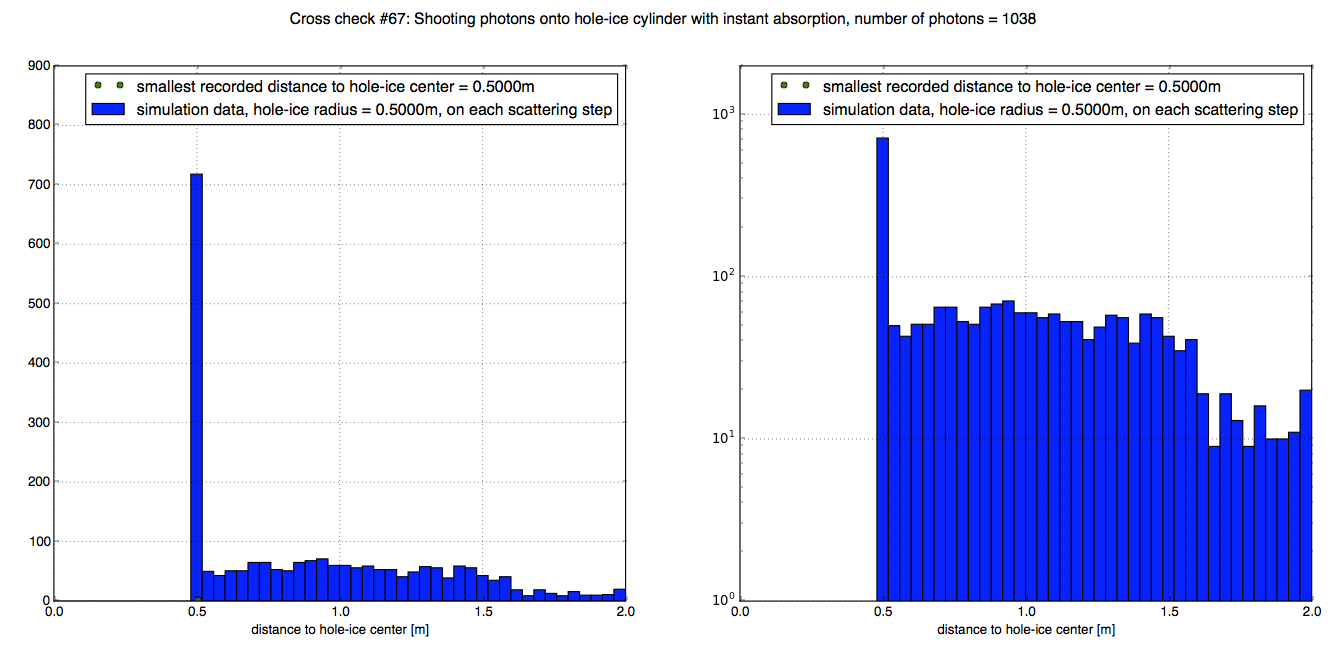
\includegraphics[width=0.32\textwidth, trim={1cm 0 25cm 2cm}, clip]{img/cross-check-67-histogram}}\hfill
  \subcaptionbox{Distance to the next scattering point and distance to hole-ice center for each scattering step.}{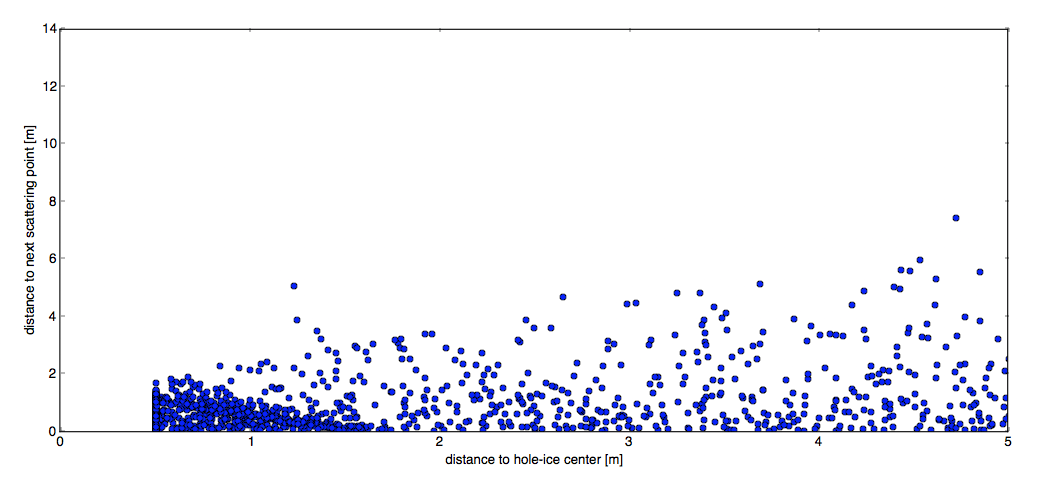
\includegraphics[width=0.65\textwidth, trim={0 0 1cm 0}, clip]{img/cross-check-67-scatter}}
  \caption{Analyzing the simulation of photons propagating towards a hole-ice cylinder configured for instant absorption. No photon can be recorded within the hole-ice cylinder's radius.}
  \label{fig:chiep7Is}
\end{figure}

\begin{figure}[htbp]
  \subcaptionbox{Starting from different positions into the same direction. View from above.}{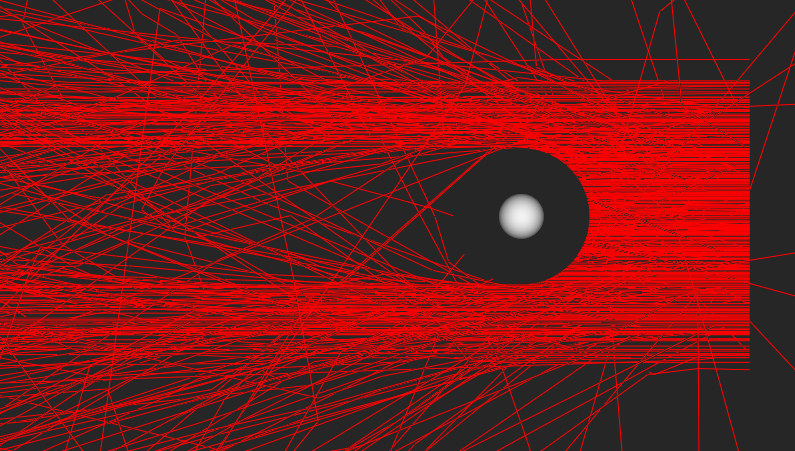
\includegraphics[width=0.49\textwidth]{img/instant-absorption-steamshovel-moo9Eiqu}}\hfill
  \subcaptionbox{Starting from the same position into different directions.}{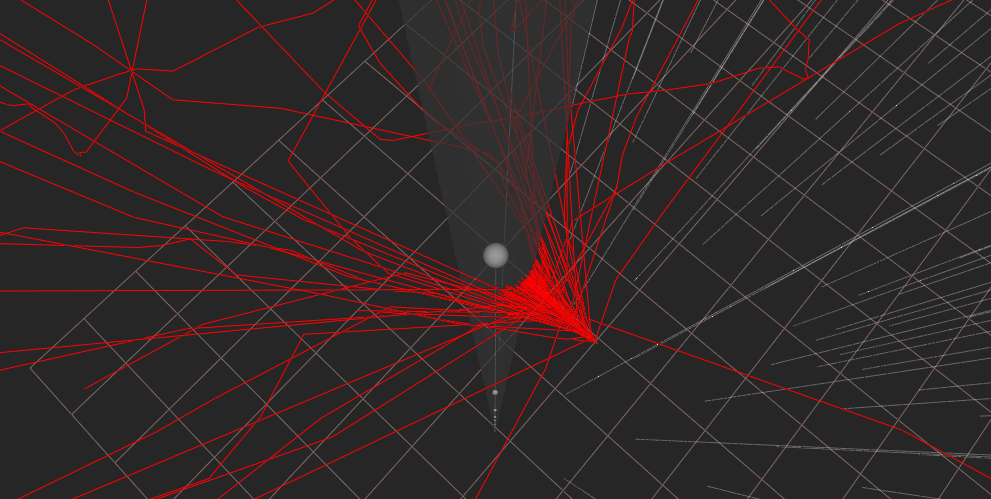
\includegraphics[width=.49\textwidth, trim={0 0 40mm 0}, clip]{img/instant-absorption-steamshovel-Zae4phei}}
  \caption{Visualizing an instant-absorption test using the \steamshovel event viewer. In the simulation, photons are started towards a cylinder configured for instant absorption. If the medium-propagation algorithm works as expected, no photon can get inside the cylinder.}
  \label{fig:moo9Eiqu}
\end{figure}

A related, but more complex scenario is starting photons within two
nested cylinders where the inner cylinder is configured for a short
scattering length and the outer cylinder is configured for instant
absorption (figure \ref{fig:sahmoo8O}).

\begin{figure}[htbp]
  \subcaptionbox{View from above.}{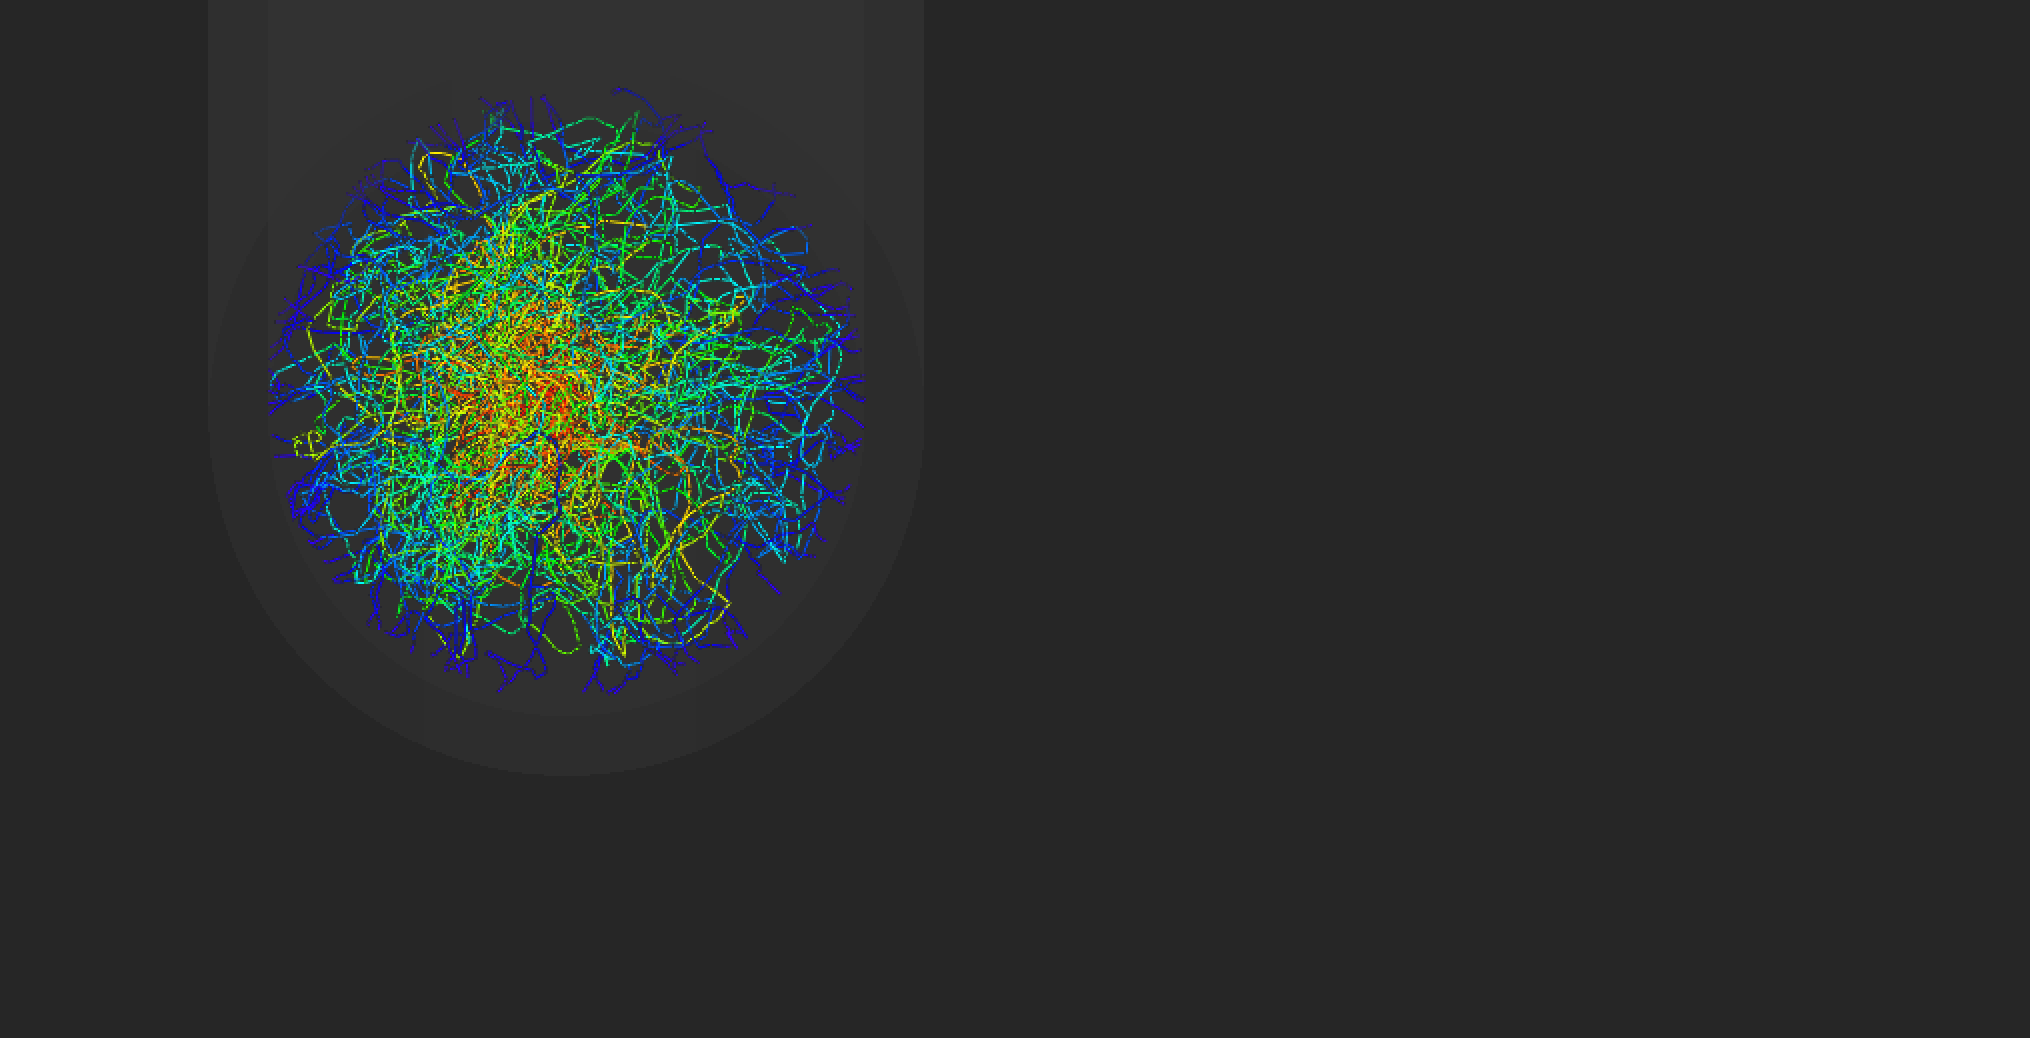
\includegraphics[width=.32\textwidth, trim={0 3cm 16cm 0}, clip]{img/instant-absorption-steamshovel-sahmoo8O-above}}\hfill
  \subcaptionbox{View from the side.}{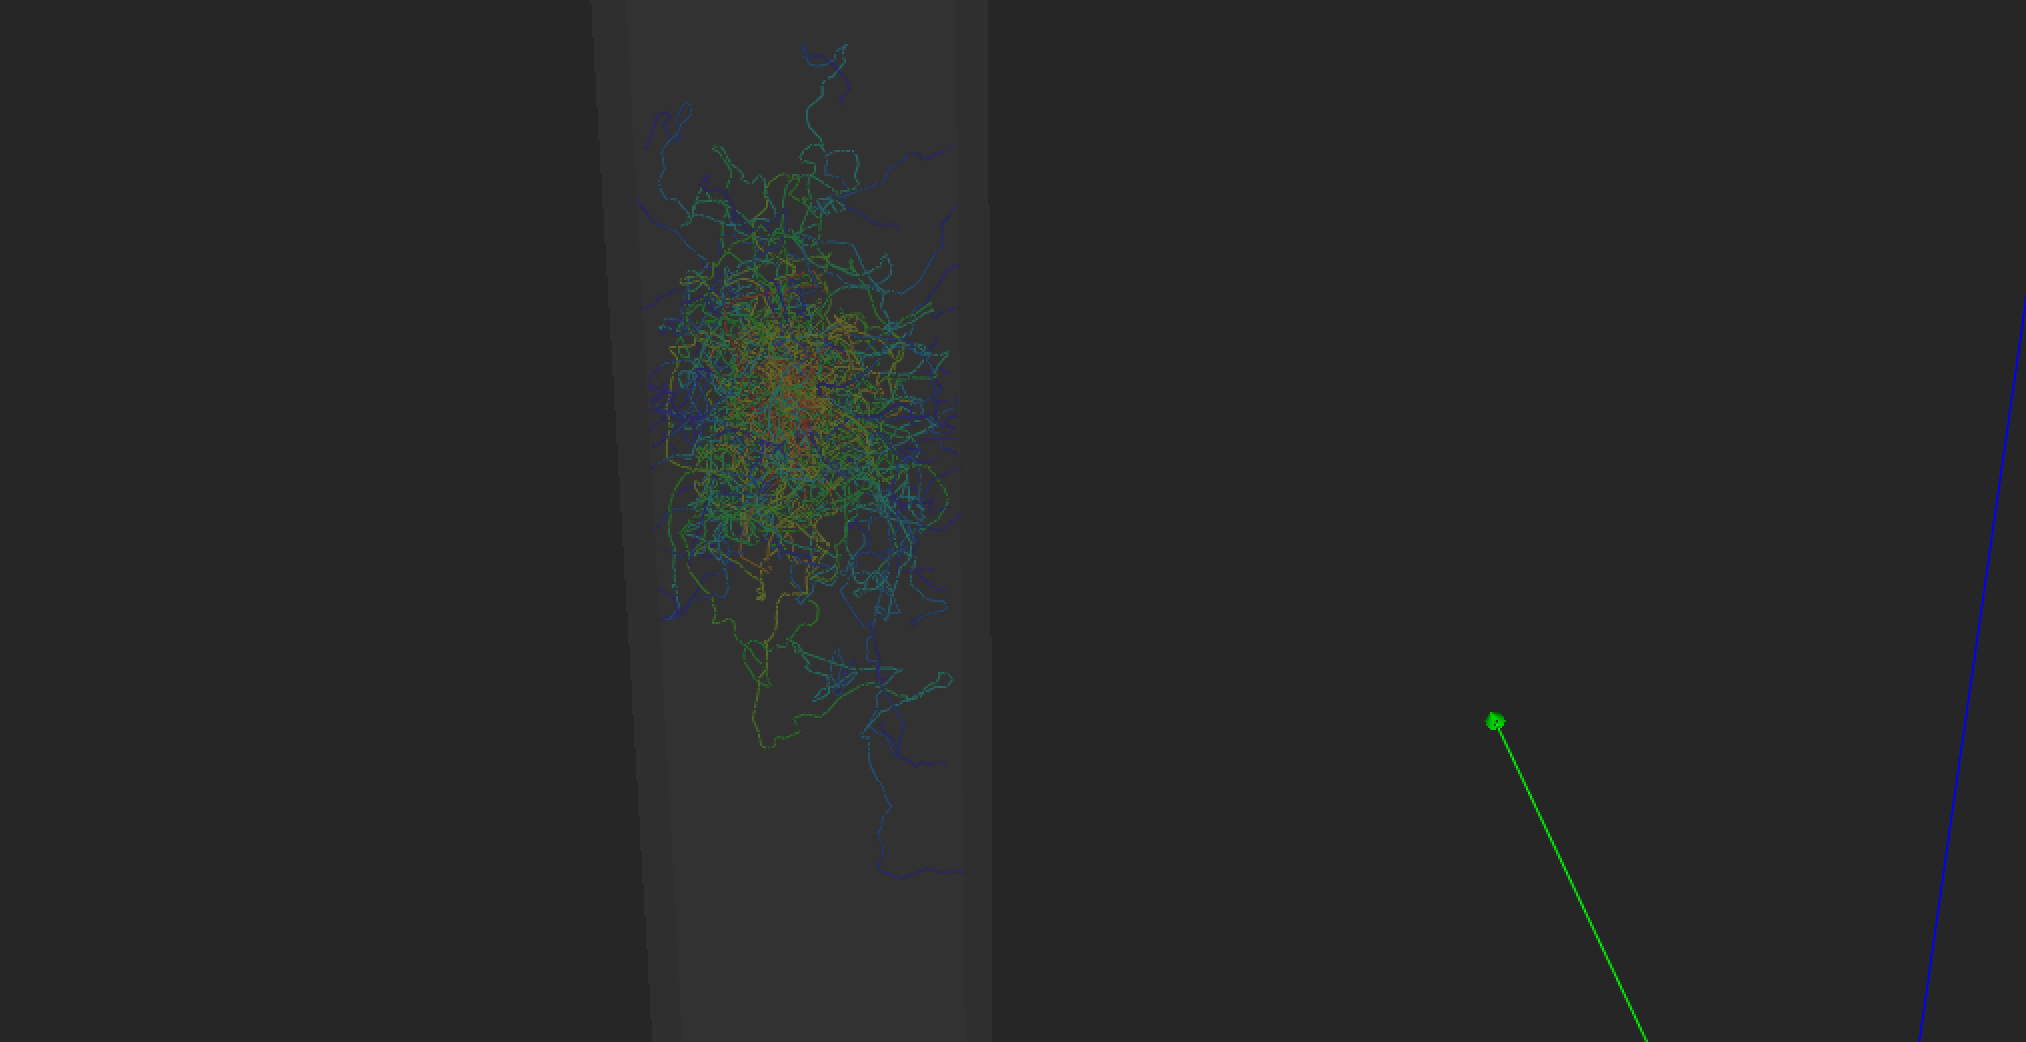
\includegraphics[width=.32\textwidth, trim={6cm 4cm 13cm 1.5cm}, clip]{img/instant-absorption-steamshovel-sahmoo8O-3d}}\hfill
  \subcaptionbox{Instant absorption of the outer cylinder turned off.}{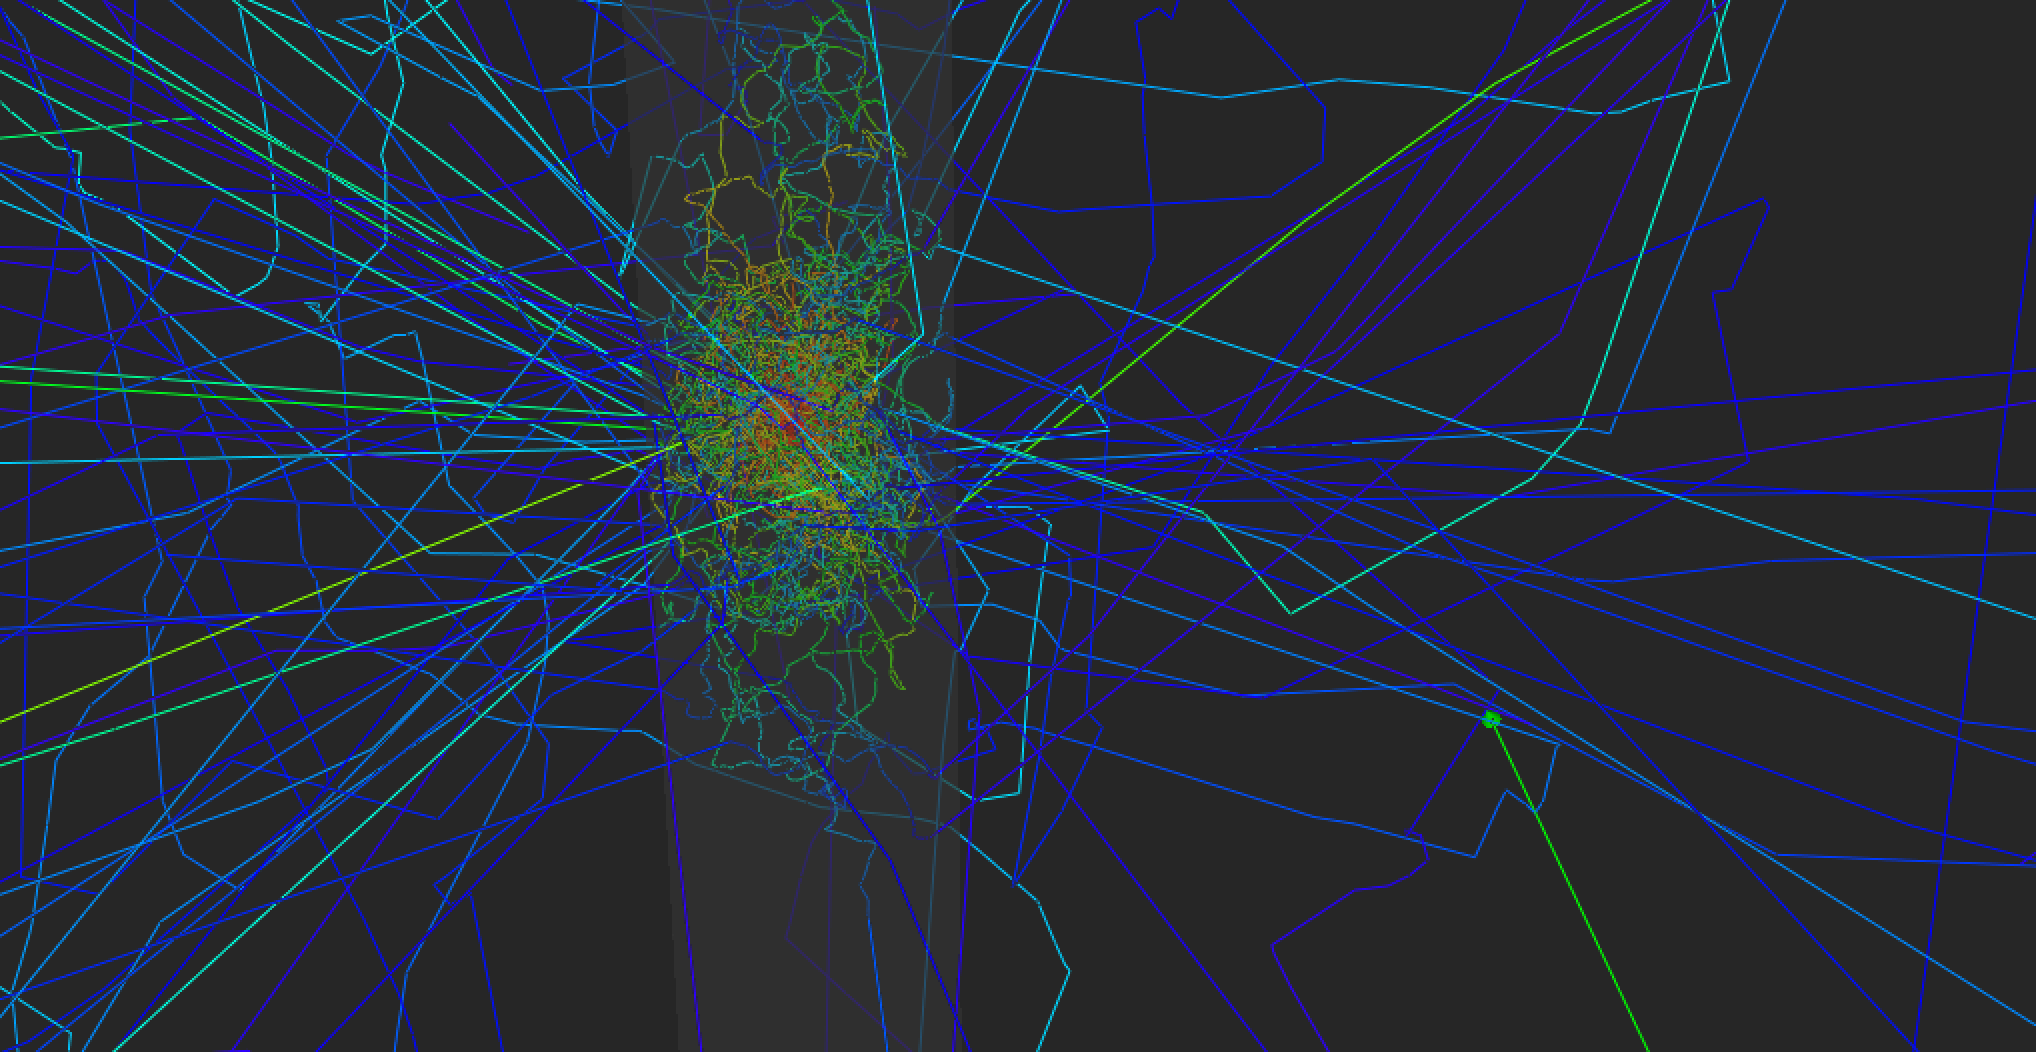
\includegraphics[width=.32\textwidth, trim={6cm 4cm 13cm 1.5cm}, clip]{img/instant-absorption-steamshovel-sahmoo8O-turned-off}}
  \caption{Visualizing an instant-absorption test where photons are started within two nested cylinders. The outer cylinder is configured for instant absorption. No photon can pass through the area between both cylinders unless the instant absorption is turned off.}
  \label{fig:sahmoo8O}
\end{figure}

\FloatBarrier\newpage
\subsubsection{Arrival-Time Distributions}
\label{sec:arrival_time}

One way to test the behavior of statistical properties of a sample of
photons is to plot the arrival-time distribution of photons traveling
from a central position to receiving optical modules around the starting
position. Figure \ref{fig:eipau6Ag} shows arrival-time distributions for
this scenario being carried out with a flasher experiment compared to
two simulations with different hole-ice configurations each.

\sourcepar{The source for the simulations and for creating these histograms can be found in \issue{91}.}

\begin{figure}[htbp]
  \subcaptionbox{Top view of the detector strings in this simulation. The photons are started at the middle optical module of string 63, and are received by the optical modules of the surrounding strings 70, 71, 64, 55, 54, and 62.}{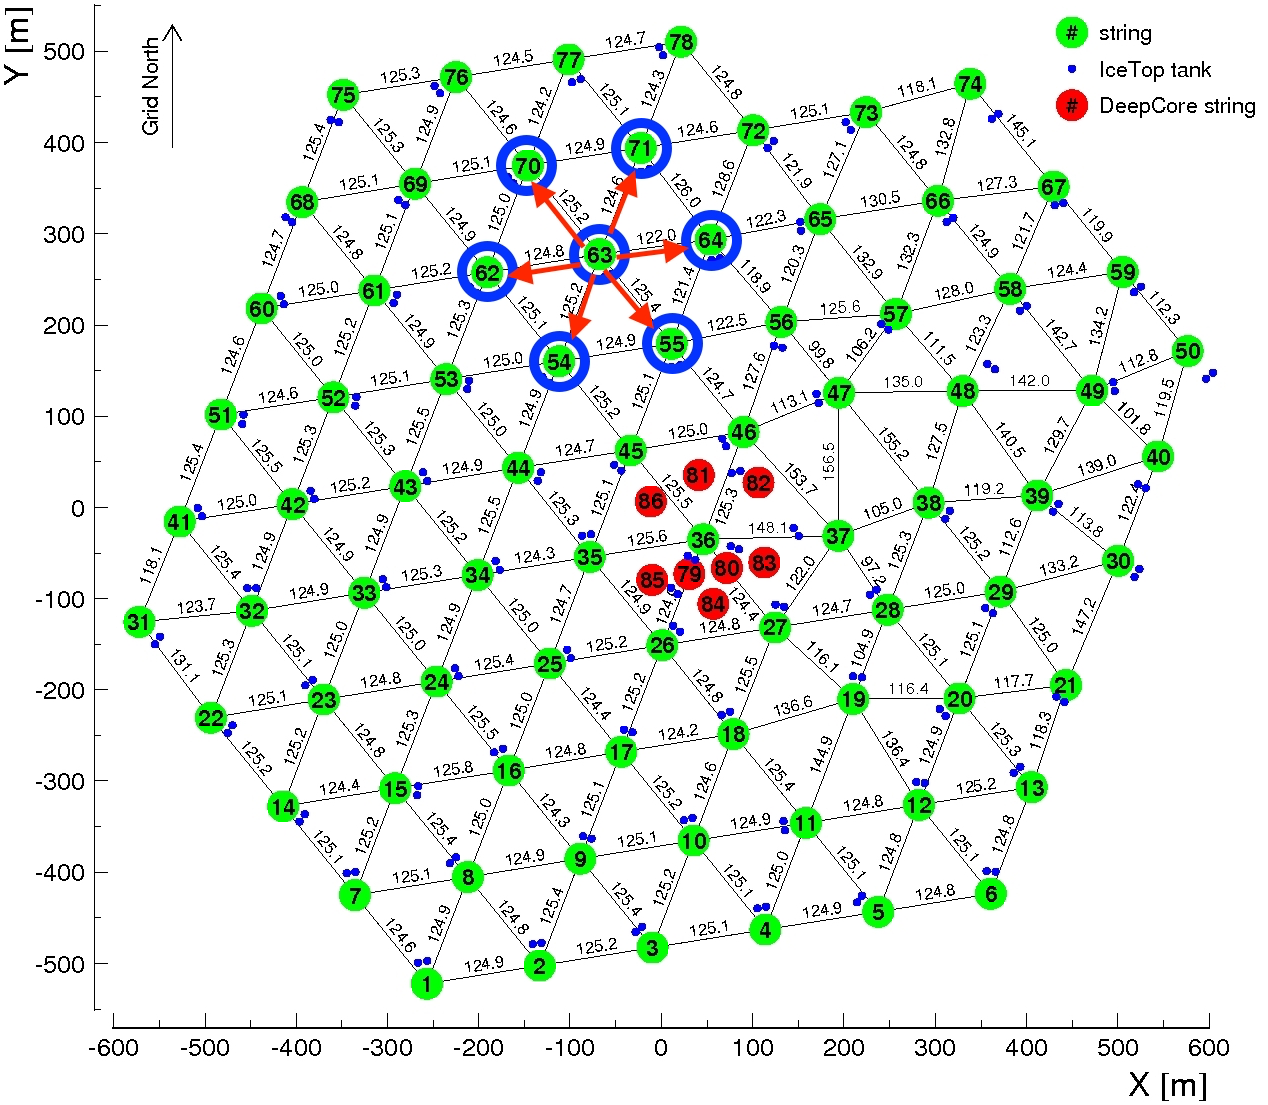
\includegraphics[width=.48\linewidth]{img/flasher-scenario}}
  \hfill
  \subcaptionbox{Photon-arrival-time distributions for different hole-ice configurations. The dashed lines indicate the mean arrival times.}{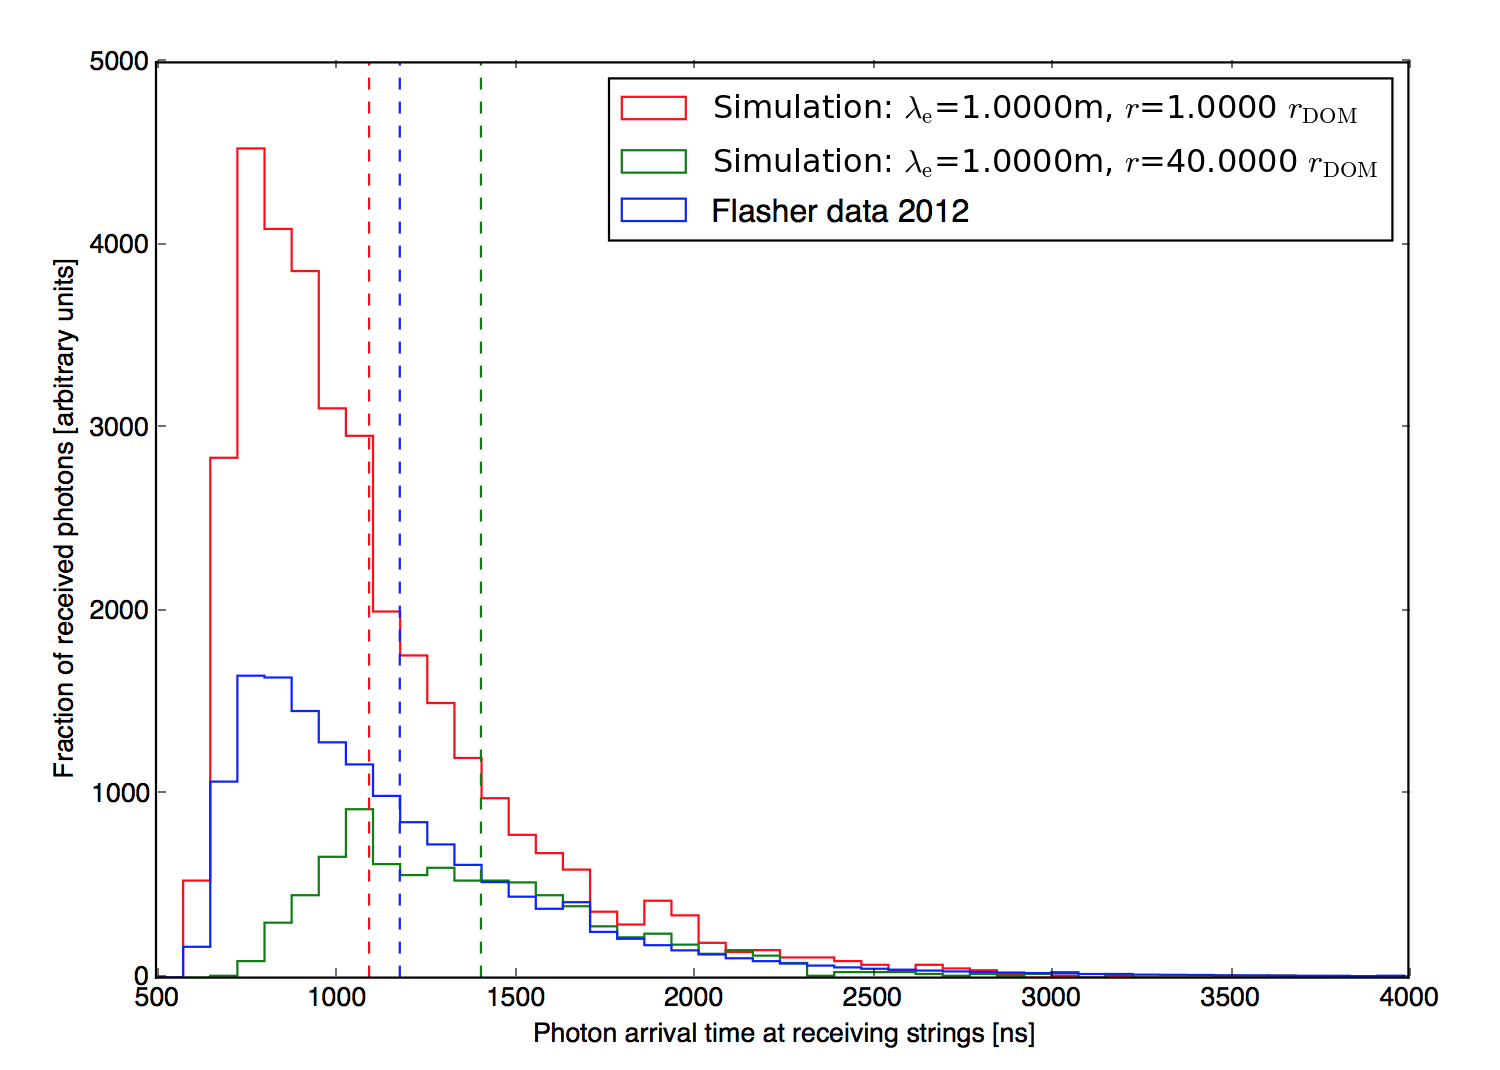
\includegraphics[width=.48\linewidth]{img/arrival-time-distribution-eipau6Ag}}
  \caption{Creating arrival-time distributions for photons propagating through hole ice. The photons are started at a central position and detected by optical modules around the starting position.}
  \label{fig:eipau6Ag}
\end{figure}

An estimation based on the mean scattering angle and the radius of the
hole-ice cylinder suggests that one would need a difference of the
hole-ice cylinder's radius of several meters to cause a difference in
the mean arrival time on the order of \(100\ns\). While this is no
realistic scenario as the drill hole's radius is only about \(50\cm\),
the simulation allows to use extreme scenarios to observe the effects
more noticeable.

From the comparison of the arrival-time distributions, note that the
distribution that is based on real data is comparable to the ones based
on simulations, which suggests that the new algorithm does not introduce
unexpected, unphysical effects to the photon propagation.

In the simulation where the hole-ice cylinders have a much larger
radius, the effects of the hole ice should be stronger. Indeed, the
comparison of the distributions shows three effects to expect from this
assumption: First, in the simulation with stronger hole-ice effect, less
photons arrive at the receiving optical modules in total as more photons
are scattered away by the hole ice. Secondly, for stronger hole ice, the
photons arrive later at the receiving optical modules, because they
spend more time scattering randomly within the hole-ice cylinder before
reaching the receiving optical module. Thirdly, for stronger hole ice,
the left-hand side of the distribution histogram is less steep, because
with more scattering points on the photon's path, there is a larger
number of possible paths, which leads to the arrival time being more
distributed.

While these effects confirm the expectations qualitatively, examining
other high-level observables allows to compare expectations to the
simulations' results even quantitatively. This is the subject of the
following sections, beginning with observing the photons' path-length
distributions.

\FloatBarrier\newpage
\subsubsection{Exponential Distribution of the Total Path Length}
\label{sec:total_path_length_distribution}

Let the \textbf{Total path length} of a photon be the summed distance
from the position where the photon is created, along the photon's path,
to the position where the photon is absorbed. The total path length
\(X\) of photons that propagate in a medium with an absorption
probability that is the same everywhere in the medium, for example
within a confined volume within the bulk ice, is expected to follow an
exponential distribution with a rate parameter corresponding to the
absorption probability, or equivalently the absorption length
\(\lambda\) within the
medium.\footnote{If the photons do not depend on each other, the number of photons that are absorbed at a certain path length does only depend on the absorption probability, or equivalently on the absorption length $\lambda$, and the number of photons remaining at this path length. When a photon is absorbed, the number of remaining photons decreases. Thus, the change in the number of photons is proportional to the number of photons, causing the number of photons absorbed at a certain path length following an exponential distribution. See also appendix \ref{sec:exponential_distribution}.}

\begin{equation}
  X: \ \ P(X \in [x; x + \dx[) \propto e^{\sfrac{-x}{\lambda}}, \ \ x \in \reals^+_0
\end{equation}

When propagating photons within a hole-ice cylinder, their path length
should also follow an exponential distribution, but with different
absorption length \(\lambda\hi\), as long as the absorption length is
sufficiently small such that most photons do not leave the cylinder
before being absorbed.

This behavior can be verified using a simulation. In the simulation, a
pencil beam of \(10^4\) photons is started within a hole-ice cylinder
with a radius of \(1.0\m\). The photons are started with a distance of
\(0.9\m\) to the cylinder center towards the cylinder center. Let the
effective scattering length within the cylinder be \(100.0\m\) and the
absorption length be \(0.1\m\). For each simulated photon, the total
path length is recorded.

\begin{figure}[htbp]
  %\smallerimage{cross-check-64-steamshovel}
  \caption{\steamshovel event display of the simulation of photons propagating and being absorbed within the hole-ice cylinder without medium transition. The photons are started within the hole-ice cylinder, which is represented by the grey cylinder, inwards. The detector module, which is represented by the white sphere in the center of the figure, is shown only to illustrate the size of the scenery and is configured not to interact with the simulated photons.}
\end{figure}

\sourcepar{The implementation of this cross check can be found in \issue{64}.}

The distribution of the total path length should follow an exponential
decay curve. From the rate of the decay, one should be able to read the
absorption length \(\lambda\) (see appendix
\ref{sec:exponential_distribution}).

\begin{figure}[htbp]
  \image{cross-check-64-exponential-distribution.png}
  \caption{Distribution of the total path length of simulated photons both started and absorbed within a hole-ice cylinder using the new medium-propagation algorithm. The distribution follows an exponential curve. The fitted absorption length is $\lambda_\text{abs}=0.1003\m \pm 0.0011\m$. The true absorption length used in the simulation is $0.1000\m$.}
  \label{fig:gieNa2Th}
\end{figure}

Indeed, the simulation yields the expected distribution of the total
path length (figure \ref{fig:gieNa2Th}). Via a curve fit, the absorption
length \(\lambdaabs\) can be determined for this simulation to be
\(\lambdaabs = 0.1003\m \pm 0.0011\m\), which is in accordance with the
true absorption length of \(0.1000\m\) used in the simulation.

\FloatBarrier\newpage
\subsubsection{Piecewise Exponential Distribution of the Total Path Length for One Medium Boundary}

This cross check aims to verify that the medium-boundary transition is
handled correctly when photons enter a hole-ice cylinder from outside.

In a simulation, a pencil beam of \(10^5\) photons is started in a
distance of \(2.0\m\) to cylinder center towards the hole-ice cylinder
with a radius of \(1.0\m\). The effective scattering length outside is
set to \(10^6\m\), inside to \(100\m\). The absorption length outside is
set to \(1.0\m\), inside to \(0.10\m\). As before, for each simulated
photon, the total path length, from the starting point of the photon
along the photon's trajectory to the point where the photon is absorbed,
is recorded.

\sourcepar{The implementation of this cross check can be found in \issue{65}.}

\begin{figure}[htbp]
  \smallerimage{cross-check-65-steamshovel}
  \caption{\steamshovel event display of the simulation of photons propagating through the hole-ice medium boundary. The photons are started outside and towards the hole-ice cylinder on the left hand side. As the scattering length within the cylinder is smaller, the photons scatter a lot more within the cylinder. The detector module is shown as a white sphere only to illustrate the size of the scenery and is configured not to interact with the simulated photons.}
\end{figure}

As the absorption lengths are different outside and inside the cylinder,
the histogram should now follow two separate exponential curves: The
left hand side of the histogram, which corresponds to the area outside
the cylinder, should follow an exponential curve governed by the
absorption length outside the cylinder. The right hand side, which
corresponds to the area within the cylinder, should follow an
exponential curve governed by the absorption length within the hole-ice
cylinder.

Note that the histogram's bins are proportional to the number
\(m(x):=\sfrac{-\d n(x)}{\dx}\) of photons that are absorbed within the
path length interval \([x; x+\dx[\), not the number \(n(x)\) of
remaining photons. Thus, the histogram is expected to show a jumping
discontinuity at the position of the medium
border.\footnote{See also appendix \ref{sec:exponential_distribution}.}

\begin{figure}[htbp]
  \image{cross-check-65-histogram}
  \caption{Distribution of the total path length of simulated photons started outside and absorbed within a hole-ice cylinder using the new medium-propagation algorithm. The distribution follows two exponential curves. The fitted absorption lengths are $\lambda_\text{abs,1} = 1.016\m \pm 0.310\m$ and $\lambda_\text{abs,2} = 0.101\m \pm 0.014\m$. The true absorption length in the simulation is set to $1.000\m$ outside, and to $0.100\m$ within the hole-ice cylinder.}
  \label{fig:iquo3Ou3}
\end{figure}

The simulation yields the expected distribution of the total path length
(figure \ref{fig:iquo3Ou3}). Via a curve fit, the absorption lengths
\(\lambda_\text{abs,1} = 1.016\m \pm 0.310\m\) and
\(\lambda_\text{abs,2} = 0.101\m \pm 0.014\m\) are in determined in
accordance with the true absorption length outside of \(1.000\m\) and
within the hole-ice cylinder of \(0.100\m\) set in the simulation.

\FloatBarrier\newpage
\subsubsection{Piecewise Exponential Distribution of the Total Path Length for Two Medium Boundaries}

This cross check aims to verify that the medium-boundary transition is
handled correctly when photons enter and leave a hole-ice cylinder.

In a simulation, a pencil beam of \(10^5\) photons is started in a
distance of \(1.5\m\) to the cylinder center towards the hole-ice
cylinder with a radius of \(0.5\m\). The effective scattering length
outside and inside is set to \(10^6\m\). The absorption length outside
is set to \(1.0\m\), inside to \(0.75\m\). As before, for each simulated
photon, the total path length is recorded.

\sourcepar{The implementation of this cross check can be found in \issue{66}.}

\begin{figure}[htbp]
  \smallerimage{cross-check-66-steamshovel}
  \caption{\steamshovel event display of the simulation of photons propagating through a hole-ice cylinder. As the scattering length is chosen to be very large, the photon path appears as a single line.  The photons are started outside the hole-ice cylinder on the left hand side. Some of them are absorbed before entering the cylinder, some within the cylinder and some after leaving the cylinder on the right hand side. The detector module is shown as a white sphere only to illustrate the size of the scenery and is configured not to interact with the simulated photons.}
\end{figure}

As the simulated photons may now cross two different medium boundaries,
the distribution of the path lengths should follow three exponential
curves: On the left hand side of the histogram, which corresponds to the
photons that are absorbed before entering the hole ice, the histogram
should follow an exponential curve governed by the absorption length
outside. In the middle, which corresponds to the photons that are
absorbed inside the cylinder, the histogram should follow an exponential
curve governed by the absorption length within the hole ice. On the
right hand side, which corresponds to the photons that are absorbed
after leaving the hole-ice cylinder, the histogram should follow an
exponential curve, again, governed by the absorption length outside the
cylinder.

\begin{figure}[htbp]
  \image{cross-check-66-histogram}
  \caption{Distribution of the total path length of simulated photons, which start outside the cylinder, and may be absorbed before, within or after passing the cylinder, using the new medium-propagation algorithm. The distribution follows three exponential curves. The fitted absorption lengths are $\lambda_\text{abs,1} = 1.02\m \pm 0.22\m$, $\lambda_\text{abs,2} = 0.68\m \pm 0.19\m$, and $\lambda_\text{abs,3} = 1.07\m \pm 0.23\m$. The true absorption length in the simulation is set to $1.00\m$ outside, and to $0.75\m$ within the hole-ice cylinder.}
  \label{fig:io9eiDee}
\end{figure}

The simulation yields the expected distribution of the total path length
(figure \ref{fig:io9eiDee}). The absorption lengths
\(\lambda_\text{abs,1} = 1.02\m \pm 0.22\m\),
\(\lambda_\text{abs,2} = 0.68\m \pm 0.19\m\) and
\(\lambda_\text{abs,3} = 1.07\m \pm 0.23\m\) determined via a curve fit
are in accordance with the true absorption length outside of \(1.00\m\)
and within the hole-ice cylinder of \(0.75\m\) set in the simulation.

\FloatBarrier
\subsubsection{Distance to Next Scattering Point in Relation to the Distance From the Hole-Ice Center}
\label{sec:cross_check_71}

The cross checks of the previous sections refer to the absorption
length. To examine the scattering-length behavior of the photons
simulated using the new media-propagation algorithm, this cross check
observes the distance to the next scattering point in relation to the
distance from the hole-ice center at each scattering point.

In a simulation, a plane wave of 100 photons is started towards a
hole-ice cylinder. Let the hole-ice radius be \(0.50\m\). The scattering
length within the hole-ice cylinder is \(0.06\m\), the scattering length
in the surrounding bulk ice is \(1.48\m\). For each scattering step, the
distance to the next scattering point and the current distance to the
center of the hole-ice cylinder are recorded.

\sourcepar{The implementation of this cross check can be found in \issue{71}.}

\begin{figure}[htbp]
  \smallerimage{cross-check-71-steamshovel}
  \caption{\steamshovel event display of a simulation of a plane wave of photons propagating towards a hole-ice cylinder. The scattering length within the hole-ice cylinder is different from the scattering length within the surrounding bulk ice.}
  \label{fig:An7ik8pu}
\end{figure}

As the distance to the next scattering point should be exponentially
distributed, governed by the scattering lengths within and without the
hole-ice cylinder, the distance to the next scattering point should
differ in the following three regions:

\begin{enumerate}
  \item Well within the hole-ice radius, the distance to the next scattering point should be in the range of the scattering length of the hole ice.
  \item Well outside the hole-ice radius, the distance to the next scattering point should be in the range of the scattering length of the surrounding bulk ice.
  \item In the vicinity of the hole-ice-cylinder radius, there should be some kind of transition due to the complex geometrical simulation.
\end{enumerate}

\begin{figure}[htbp]
  \centering
  \subcaptionbox{All data points}{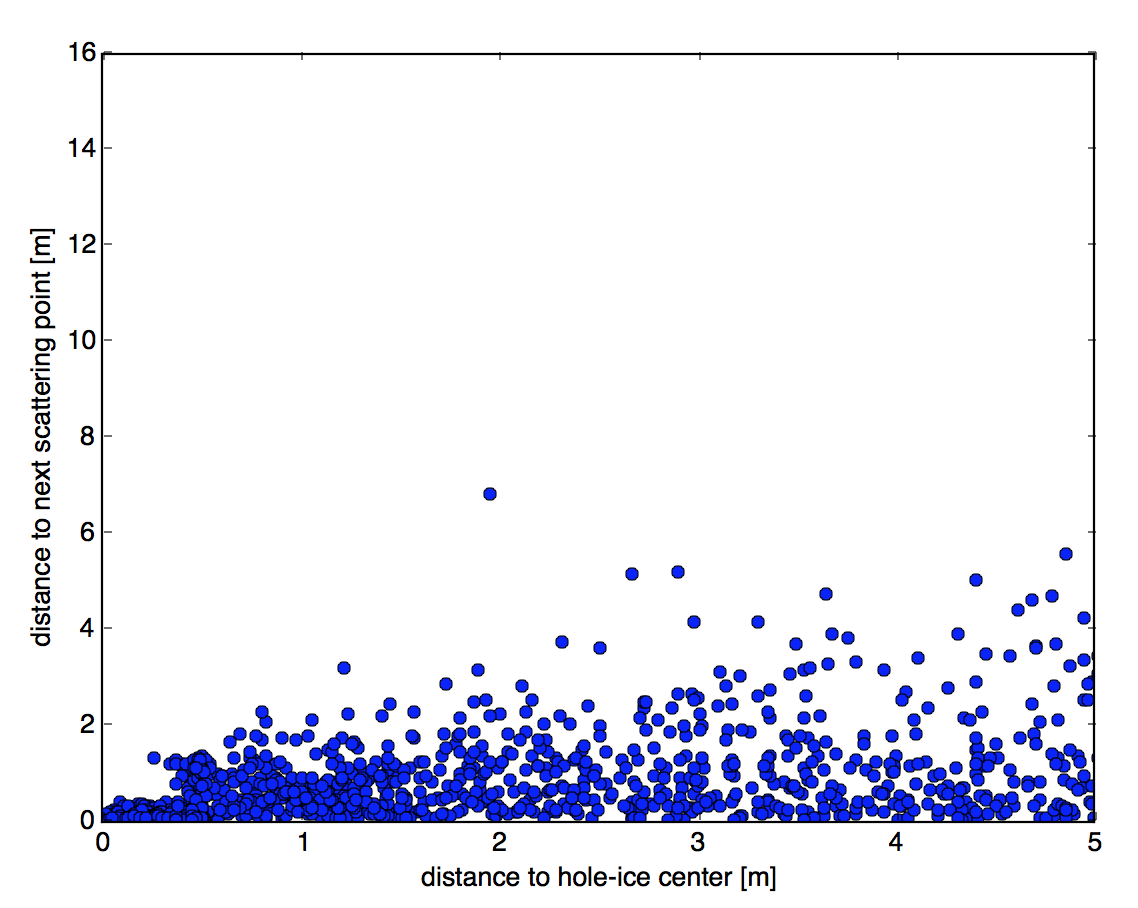
\includegraphics[width=0.48\linewidth]{img/cross-check-71-scatter}}\hfill
  \subcaptionbox{Averaged for bins of a width of  $10\cm$}{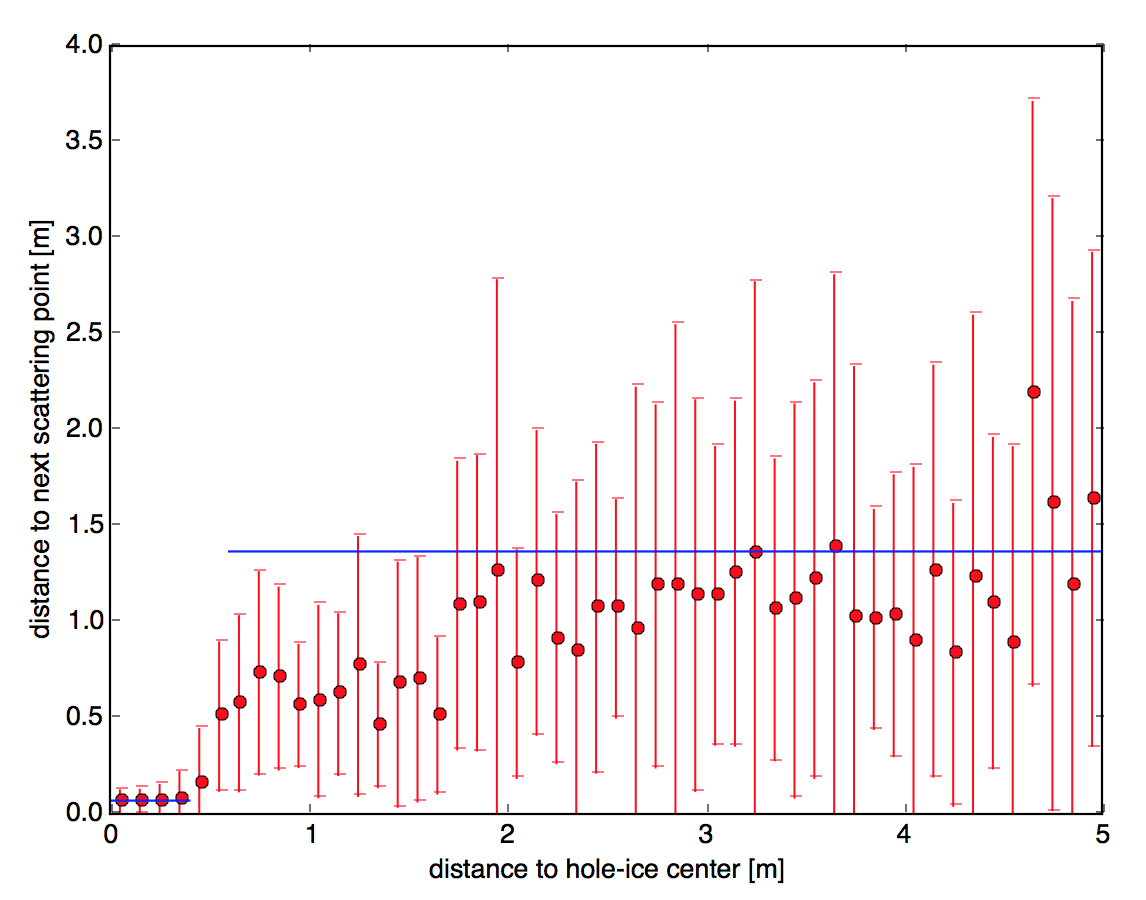
\includegraphics[width=0.48\linewidth]{img/cross-check-71-bins}}\hfill
  \subcaptionbox{Magnification of the vicinity of the hole-ice border}{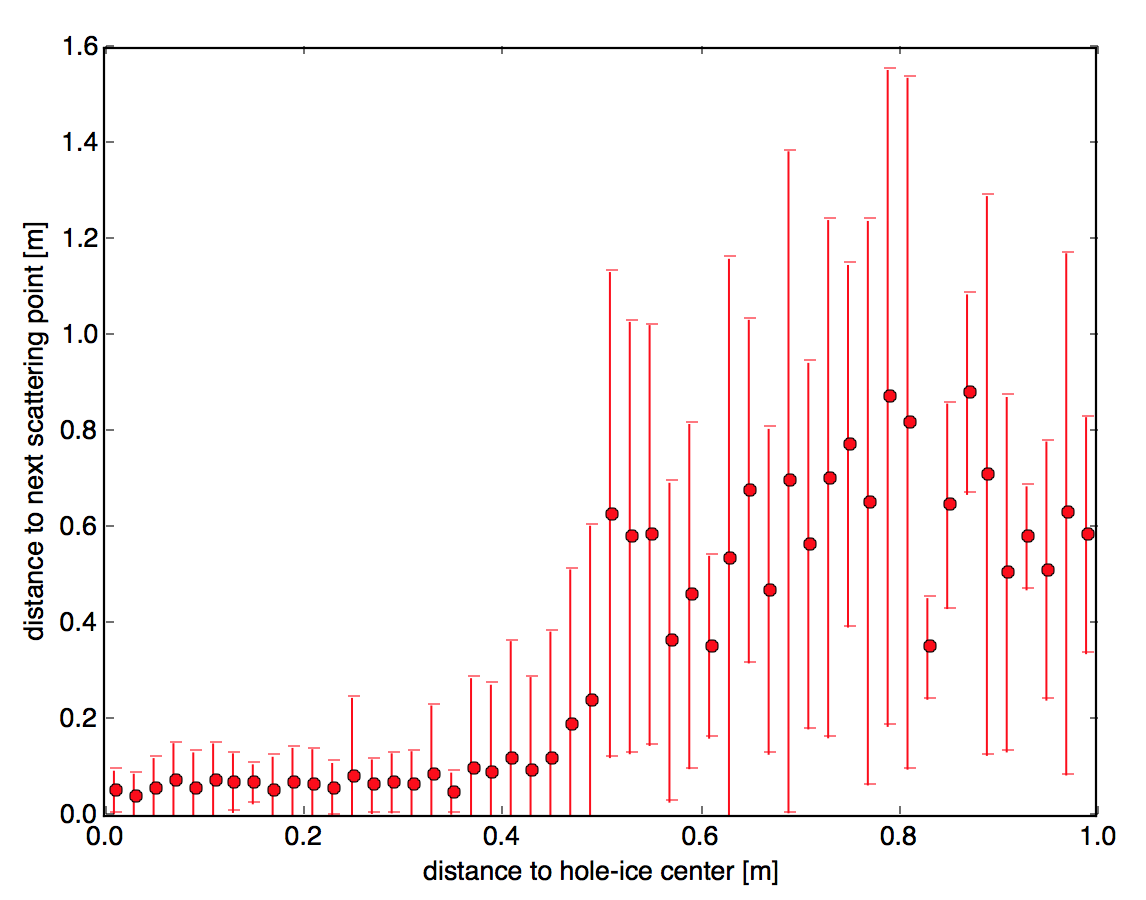
\includegraphics[width=0.48\linewidth]{img/cross-check-71-bins-vicinity}}
  \caption{For each scattering step of a simulation of photons entering a hole-ice cylinder, plot the distance to the next scattering step in relation to the current distance to the cylinder center. The mean distance to the next scattering point within $80\,\%$ of the hole-ice radius is fitted to $0.07\m \pm 0.07\m$. The mean distance to the next scattering point outside of $120\,\%$ of the hole-ice radius is fitted to $1.37\m\pm 1.37\m$. The true scattering length in the simulation is set to $0.06\m$ inside, and to $1.48\m$ outside the hole-ice cylinder.}
  \label{fig:eeYoid2p}
\end{figure}

Assuming an exponential distribution of the distance to the next
scattering point, the mean distance to the next scattering point within
\(80\,\%\) of the hole-ice radius is fitted to \(0.07\m \pm 0.07\m\),
the mean distance to the next scattering point outside of \(120\,\%\) of
the hole-ice radius is fitted to \(1.37\m\pm 1.37\m\) (figure
\ref{fig:eeYoid2p} b), which is in the range of the true scattering
lengths of \(0.06\m\) and \(1.48\m\) inside and outside the hole ice
respectively.

When plotting the local average of the distance to the next scattering
point for the vicinity of the hole-ice border (figure \ref{fig:eeYoid2p}
c), the curve shows no abrupt jump but a transition between both domains
as expected.


  \include{text/gliederung}


  %\include{text/cross_checks}
  %\include{text/likelihood}
  %\subsection{Hole Ice Trajectory
Corrections}\label{hole-ice-trajectory-corrections}

Consider a random photon trajectory through the ice. The photon is
created by a particle interaction at the starting point of the
trajectory. On its way, the photon is scattered several times within the
ice before it is absorbed and thereby detected in one of IceCube's DOMs.

\image{photon-trajectory-oheeL3ai.pdf}

\begin{itemize}
\item
  Consider path of photon through ice.
\item
  Interaction propability determined by ice properties and photon
  wavelength.
\item
  Interaction points determined by these properties and random process.
\item
  Look at part of this trajectory, A B between two interactions.
\item
  Change scenario by adding hole ice cylinder.
\item
  Determine how the trajectory is affected by this.
\item
  Consider a photon trajectory through the ice that partially goes
  through hole ice.
\item
  Within hole ice, the ice properties are different from outside.
\item
  Most notably, the impurities (dirt) cause the photons to scatter or be
  absorbed more often there.
\item
  I.e. Scattering and absorption coefficients are larger within hole
  ice.
\item
  Correspondingly, the scattering and absorption lengths, which are the
  mean free distances until scattering or absorption, are shorter.
\end{itemize}

\image{photon-trajectory-aiph6ahD.pdf}

\begin{itemize}
\tightlist
\item
  Consider simulation of a photon.
\item
  \(A\) is the last point of interaction, i.e.~fixed.
\item
  \(B\) is determined by random process.
\item
  Consider a scenario where a photon trajectory starts at point \(A\)
  and ends at point \(B\), where it is scattered or absorbed. The photon
  does not interact inbetween \(A\) and \(B\).
\end{itemize}

\image{photon-trajectory-Edahi9sh.pdf}

\begin{itemize}
\tightlist
\item
  Now, change scenario: add hole ice cylinder.
\item
  Due to locally increased interaction coefficients, the free path is
  shorter, i.e.~modified \(B\).
\item
  Why is the path shorter?
\item
  B is determined by random variable.
\item
  If the mean free path is shorter (because the likelyhood if
  interaction is larger), then the random variable is smaller.
\item
  The change is \(\Delta b:= \overline{AB'} - \overline{AB}\).
\end{itemize}

  %\section{Problems}\label{problems}

\begin{itemize}
\tightlist
\item
  numerical issues where dependent information are calculated using
  different formulae. Methematically, both ways must lead to the same
  result; but numerically, both can differ, which leads to conflicts in
  the simulation. See 2018-01-16.
\item
  \textbf{Sonderfall: Teilchen fliegt in z-Richtung}: Diesen Fall habe
  ich die ganze Zeit über nicht berücksichtigt und lasse das auch
  einstweilen bleiben. (2018-01-16)
\end{itemize}

  %
  \printbibliography
  %
  \appendix
  \section{Appendix}
  %!TEX root = ../diplomarbeit.tex

\subsection{How to Install the Modified \clsim}
\label{sec:howtoclsim}

This study needs a modified version of \clsim that does support hole-ice simulations. Until this modified version has been merged into the main \icecube Simulation Framework source code, these patched version needs to be installed manually.

\begin{bash}
# Get clsim fork
git clone git@github.com:fiedl/clsim.git $SCRATCH/clsim
cd $SCRATCH/clsim

# Symlink it into the icesim source
cd $ICESIM_ROOT/src
rm -rf clsim
ln -s $SCRATCH/clsim clsim

# Compile it
cd $ICESIM_ROOT/build
make -j 6
\end{bash}

\docframe{
\docparwithoutframe{Detailed instructions on how to install the software on the Zeuthen computing center can be found at \url{https://github.com/fiedl/hole-ice-study/blob/master/notes/2018-01-23_Installing_IceSim_in_Zeuthen.md\#install-patched-clsim}.}\medskip

\docparwithoutframe{Instructions on how to install the software locally on macOS can be found at \url{https://github.com/fiedl/hole-ice-study/blob/master/notes/2016-11-15_Installing_IceSim_on_macOS_Sierra.md}.}
}
  %!TEX root = ../diplomarbeit.tex

\subsection{Source Code of Algorithm A}
\label{sec:algorithm_a_source}

This is the source code of the first propagation algorithm through different media, described in section \ref{sec:algorithm_a}.

\sourcepar{The source code can also be found online at \url{https://github.com/fiedl/clsim/tree/sf/hole-ice-2017/resources/kernels/lib}.}

\begin{ccode}
// https://github.com/fiedl/clsim/blob/sf/hole-ice-2017/resources/kernels/lib/hole_ice/hole_ice.c

#ifndef HOLE_ICE_C
#define HOLE_ICE_C

#include "hole_ice.h"
#include "../intersection/intersection.c"

inline bool is_between_zero_and_one(floating_t a) {
  return ((!my_is_nan(a)) && (a > 0.0) && (a < 1.0));
}

inline bool not_between_zero_and_one(floating_t a) {
  return (! is_between_zero_and_one(a));
}

inline unsigned int number_of_medium_changes(HoleIceProblemParameters_t p)
{
  // These are ordered by their frequency of occurrance in order
  // to optimize for performance.
  if (not_between_zero_and_one(p.entry_point_ratio) && not_between_zero_and_one(p.termination_point_ratio)) return 0;
  if (not_between_zero_and_one(p.entry_point_ratio) || not_between_zero_and_one(p.termination_point_ratio)) return 1;
  if (p.entry_point_ratio == p.termination_point_ratio) return 0; // tangent
  return 2;
}

inline floating_t hole_ice_distance_correction(HoleIceProblemParameters_t p)
{
  // Depending on the fraction of the distance the photon is traveling
  // within the hole ice, there are six cases to consider.
  //
  // N  denotes the number of intersections.
  // H  means that the trajectory starts within hole ice.
  // !H means that the trajectory starts outside of the hole ice.
  //
  // Case 1: The trajectory is completely outside of the hole ice (!H, N=0).
  // Case 2: The trajectory is completely within the hole ice (H, N=0).
  // Case 3: The trajectory begins outside, but ends inside the hole ice (!H, N=1).
  // Case 4: The trajectory begins inside, but ends outside the hole ice (H, N=1).
  // Case 5: The trajectory starts and ends outside, but passes through the hole ice (!H, N=2).
  // Case 6: The trajectory begins within one hole-ice cylinder, passes through
  //           normal ice and ends in another hole-ice cylinder (H, N=2).
  //
  // For further information, please have look at:
  // https://github.com/fiedl/clsim/tree/sf/master/resources/kernels/lib/hole_ice

  const unsigned int num_of_medium_changes = number_of_medium_changes(p);

  // Case 1: The trajectory is completely outside of the hole ice.
  // Thus, needs no correction.
  if ((num_of_medium_changes == 0) && !p.starts_within_hole_ice) {
    return 0;
  }

  const floating_t ac = p.distance * p.termination_point_ratio;

  if (p.starts_within_hole_ice) {

    // Case 4: The trajectory begins inside, but ends outside the hole ice.
    if (p.interaction_length_factor * p.distance > ac) {
      return (1.0 - 1.0 / p.interaction_length_factor) * ac;

    // Case 2: The trajectory is completely within the hole ice.
    } else {
      return (p.interaction_length_factor - 1.0) * p.distance;
    }

  } else {

    const floating_t yb = p.distance * (1.0 - p.entry_point_ratio);
    floating_t yc = p.distance * (p.termination_point_ratio - p.entry_point_ratio);

    if (yc < 0) {
      printf("WARNING: YC SHOULD NOT BE NEGATIVE, BUT YC=%f\n", yc);
      yc = 0;
    }

    // Case 5: The trajectory starts and ends outside, but passes through the hole ice.
    if (p.interaction_length_factor * yb > yc) {
      return (1.0 - 1.0 / p.interaction_length_factor) * yc;

    // Case 3
    } else {
      return (p.interaction_length_factor - 1.0) * p.distance * (1.0 - p.entry_point_ratio);
    }
  }

#ifdef PRINTF_ENABLED
  printf("WARNING: UNHANDLED INTERSECTION CASE. This point should not be reached.");
#endif

  return my_nan();
}

inline floating_t hole_ice_distance_correction_for_intersection_problem(floating_t distance, floating_t interaction_length_factor, IntersectionProblemParameters_t p)
{
  calculate_intersections(&p);
  HoleIceProblemParameters_t hip = {
    distance,
    interaction_length_factor,
    intersection_s1(p), // entry_point_ratio
    intersection_s2(p), // termination_point_ratio
    intersecting_trajectory_starts_inside(p) // starts_within_hole_ice
  };
  return hole_ice_distance_correction(hip);
}

#ifdef HOLE_ICE_TEST_H
inline floating_t apply_hole_ice_correction(floating4_t photonPosAndTime, floating4_t photonDirAndWlen, unsigned int numberOfCylinders, floating4_t *cylinderPositionsAndRadii, floating_t holeIceScatteringLengthFactor, floating_t holeIceAbsorptionLengthFactor, floating_t *distancePropagated, floating_t *distanceToAbsorption)
#endif
#ifndef HOLE_ICE_TEST_H
inline floating_t apply_hole_ice_correction(floating4_t photonPosAndTime, floating4_t photonDirAndWlen, unsigned int numberOfCylinders, __constant floating4_t *cylinderPositionsAndRadii, floating_t holeIceScatteringLengthFactor, floating_t holeIceAbsorptionLengthFactor, floating_t *distancePropagated, floating_t *distanceToAbsorption)
#endif
{

  if (!(my_is_nan(photonPosAndTime.x) || my_is_nan(*distancePropagated))) {

    // Find out which cylinders are in range in a separate loop
    // in order to improve parallelism and thereby performance.
    //
    // See: https://github.com/fiedl/hole-ice-study/issues/30
    //
    #ifdef NUMBER_OF_CYLINDERS
      // When running this on OpenCL, defining arrays using a constant
      // as array size is not possible. Therefore, we need to use a
      // pre-processor makro here.
      //
      // See: https://github.com/fiedl/hole-ice-study/issues/38
      //
      int indices_of_cylinders_in_range[NUMBER_OF_CYLINDERS];
    #else
      int indices_of_cylinders_in_range[numberOfCylinders];
    #endif
    {
      unsigned int j = 0;
      for (unsigned int i = 0; i < numberOfCylinders; i++) {
        indices_of_cylinders_in_range[i] = -1;
      }
      for (unsigned int i = 0; i < numberOfCylinders; i++) {
        if (sqr(photonPosAndTime.x - cylinderPositionsAndRadii[i].x) +
            sqr(photonPosAndTime.y - cylinderPositionsAndRadii[i].y) <=
            sqr(*distancePropagated + cylinderPositionsAndRadii[i].w /* radius */))
        {

          // If the cylinder has a z-range check if we consider that cylinder
          // to be in range. https://github.com/fiedl/hole-ice-study/issues/34
          //
          if ((cylinderPositionsAndRadii[i].z == 0) || ((cylinderPositionsAndRadii[i].z != 0) && !(((photonPosAndTime.z < cylinderPositionsAndRadii[i].z - 0.5) && (photonPosAndTime.z + *distancePropagated * photonDirAndWlen.z < cylinderPositionsAndRadii[i].z - 0.5)) || ((photonPosAndTime.z > cylinderPositionsAndRadii[i].z + 0.5) && (photonPosAndTime.z + *distancePropagated * photonDirAndWlen.z > cylinderPositionsAndRadii[i].z + 0.5)))))
          {
            indices_of_cylinders_in_range[j] = i;
            j += 1;
          }
        }
      }
    }

    // Now loop over all cylinders in range and calculate corrections
    // for `distancePropagated` and `distanceToAbsorption`.
    //
    for (unsigned int j = 0; j < numberOfCylinders; j++) {
      const int i = indices_of_cylinders_in_range[j];
      if (i == -1) {
        break;
      } else {

        IntersectionProblemParameters_t p = {

          // Input values
          photonPosAndTime.x,
          photonPosAndTime.y,
          cylinderPositionsAndRadii[i].x,
          cylinderPositionsAndRadii[i].y,
          cylinderPositionsAndRadii[i].w, // radius
          photonDirAndWlen,
          *distancePropagated,

          // Output values (will be calculated)
          0, // discriminant
          0, // s1
          0  // s2

        };

        calculate_intersections(&p);

        // Are intersection points possible?
        if (intersection_discriminant(p) > 0) {

          const floating_t scatteringEntryPointRatio = intersection_s1(p);
          const floating_t scatterintTerminationPointRatio = intersection_s2(p);

          HoleIceProblemParameters_t scatteringCorrectionParameters = {
            *distancePropagated,
            holeIceScatteringLengthFactor,
            scatteringEntryPointRatio,
            scatterintTerminationPointRatio,
            intersecting_trajectory_starts_inside(p)
          };

          const floating_t scaCorrection = hole_ice_distance_correction(scatteringCorrectionParameters);
          *distancePropagated += scaCorrection;

          // For the absorption, there are special cases where the photon is scattered before
          // reaching either the first or the second absorption intersection point.
          floating_t absorptionEntryPointRatio;
          floating_t absorptionTerminationPointRatio;
          floating_t absCorrection = 0.0;
          if (!(not_between_zero_and_one(scatteringCorrectionParameters.entry_point_ratio) && !scatteringCorrectionParameters.starts_within_hole_ice)) {
            // The photon reaches the hole ice, i.e. the absorption correction
            // needs to be calculated.
            p.distance = *distanceToAbsorption;
            calculate_intersections(&p);

            // If the photon is scattered away before reaching the far and of
            // the hole ice, the affected trajectory is limited by the
            // point where the photon is scattered away.
            absorptionEntryPointRatio = intersection_s1(p);
            absorptionTerminationPointRatio = min(
              *distancePropagated / *distanceToAbsorption,
              intersection_s2(p)
            );

            HoleIceProblemParameters_t absorptionCorrectionParameters = {
              *distanceToAbsorption,
              holeIceAbsorptionLengthFactor,
              absorptionEntryPointRatio,
              absorptionTerminationPointRatio,
              intersecting_trajectory_starts_inside(p),
            };

            absCorrection = hole_ice_distance_correction(absorptionCorrectionParameters);

          }
          *distanceToAbsorption += absCorrection;

        }

      }
    }
  }

}

#endif
\end{ccode}

\begin{ccode}
// https://github.com/fiedl/clsim/blob/sf/hole-ice-2017/resources/kernels/lib/hole_ice/hole_ice.h

#ifndef HOLE_ICE_H
#define HOLE_ICE_H

typedef struct HoleIceProblemParameters {
  floating_t distance;
  floating_t interaction_length_factor;
  floating_t entry_point_ratio;
  floating_t termination_point_ratio;
  bool starts_within_hole_ice;
} HoleIceProblemParameters_t;

#endif
\end{ccode}

\begin{ccode}
// https://github.com/fiedl/clsim/blob/sf/hole-ice-2017/resources/kernels/lib/intersection/intersection.c

#include "intersection.h"

inline void calculate_intersections(IntersectionProblemParameters_t *p)
{
  // Step 1
  const floating4_t vector_AM = {p->mx - p->ax, p->my - p->ay, 0.0, 0.0};
  const floating_t xy_projection_factor = my_sqrt(1 - sqr(p->direction.z));
  const floating_t length_AMprime = dot(vector_AM, p->direction) / xy_projection_factor;

  // Step 2
  p->discriminant = sqr(p->r) - dot(vector_AM, vector_AM) + sqr(length_AMprime);

  // Step 3
  const floating_t length_XMprime = my_sqrt(p->discriminant);

  // Step 4
  const floating_t length_AX1 = length_AMprime - length_XMprime;
  const floating_t length_AX2 = length_AMprime + length_XMprime;
  p->s1 = length_AX1 / p->distance / xy_projection_factor;
  p->s2 = length_AX2 / p->distance / xy_projection_factor;
}

inline floating_t intersection_s1(IntersectionProblemParameters_t p)
{
  return p.s1;
}

inline floating_t intersection_s2(IntersectionProblemParameters_t p)
{
  return p.s2;
}

inline floating_t intersection_discriminant(IntersectionProblemParameters_t p)
{
  return p.discriminant;
}

inline floating_t intersection_x1(IntersectionProblemParameters_t p)
{
  if ((p.s1 > 0) && (p.s1 < 1))
    return p.ax + p.direction.x * p.distance * p.s1;
  else
    return my_nan();
}

inline floating_t intersection_x2(IntersectionProblemParameters_t p)
{
  if ((p.s2 > 0) && (p.s2 < 1))
    return p.ax + p.direction.x * p.distance * p.s2;
  else
    return my_nan();
}

inline floating_t intersection_y1(IntersectionProblemParameters_t p)
{
  if ((p.s1 > 0) && (p.s1 < 1))
    return p.ay + p.direction.y * p.distance * p.s1;
  else
    return my_nan();
}

inline floating_t intersection_y2(IntersectionProblemParameters_t p)
{
  if ((p.s2 > 0) && (p.s2 < 1))
    return p.ay + p.direction.y * p.distance * p.s2;
  else
    return my_nan();
}

inline bool intersecting_trajectory_starts_inside(IntersectionProblemParameters_t p)
{
  return (intersection_s1(p) <= 0) &&
      (intersection_s2(p) > 0) &&
      (intersection_discriminant(p) > 0);
}

inline bool intersecting_trajectory_starts_outside(IntersectionProblemParameters_t p)
{
  return ( ! intersecting_trajectory_starts_inside(p));
}

inline bool intersecting_trajectory_ends_inside(IntersectionProblemParameters_t p)
{
  return (intersection_s1(p) < 1) &&
      (intersection_s2(p) >= 1) &&
      (intersection_discriminant(p) > 0);
}
\end{ccode}

\begin{ccode}
// https://github.com/fiedl/clsim/blob/sf/hole-ice-2017/resources/kernels/lib/intersection/intersection.h

#ifndef INTERSECTION_H
#define INTERSECTION_H

typedef struct IntersectionProblemParameters {

  // Input values
  //
  floating_t ax;
  floating_t ay;
  floating_t mx;
  floating_t my;
  floating_t r;
  floating4_t direction;
  floating_t distance;

  // Output values, which will be calculated in
  // `calculate_intersections()`.
  //
  floating_t discriminant;
  floating_t s1;
  floating_t s2;

} IntersectionProblemParameters_t;

#endif
\end{ccode}


  %!TEX root = ../diplomarbeit.tex

\subsection{Source code of Algorithm B}
\label{sec:algorithm_b_source}

This is the source code of the second propagation algorithm through different media, described in section \ref{sec:algorithm_b}.

\sourcepar{The source code can also be found online at \url{https://github.com/fiedl/clsim/tree/sf/hole-ice-2018/resources/kernels/lib}.}

\begin{ccode}
// https://github.com/fiedl/clsim/blob/sf/hole-ice-2018/resources/kernels/lib/propagation_through_media/propagation_through_media.c

#ifndef PROPAGATION_THROUGH_MEDIA_C
#define PROPAGATION_THROUGH_MEDIA_C

#include "propagation_through_media.h"
#include "../ice_layers/ice_layers.c"
#ifdef HOLE_ICE
  #include "../hole_ice/hole_ice.c"
#endif


// PROPAGATION THROUGH DIFFERENT MEDIA 2018: Layers, Cylinders
// -----------------------------------------------------------------------------

// We know how many scattering lengths (`sca_step_left`) and
// absorption lengths (`abs_lens_left`) the photon will
// travel in this step.
//
// Because the mean scattering and absorption lengths are local
// properties, i.e. depend on the ice layer or whether the photon
// is within a hole-ice cylinder, we need to convert `sca_step_left`
// and `abs_lens_left` to geometrical distances in order to determine
// where the next interaction point is, i.e. how far to propagate
// the photon in this step.

inline void apply_propagation_through_different_media(
  floating4_t photonPosAndTime, floating4_t photonDirAndWlen,
  #ifdef HOLE_ICE
    unsigned int numberOfCylinders, __constant floating4_t *cylinderPositionsAndRadii,
    __constant floating_t *cylinderScatteringLengths, __constant floating_t *cylinderAbsorptionLengths,
  #endif
  floating_t *distances_to_medium_changes, floating_t *local_scattering_lengths, floating_t *local_absorption_lengths,
  floating_t *sca_step_left, floating_t *abs_lens_left,
  floating_t *distancePropagated, floating_t *distanceToAbsorption)
{

  int number_of_medium_changes = 0;
  distances_to_medium_changes[0] = 0.0;
  int currentPhotonLayer = min(max(findLayerForGivenZPos(photonPosAndTime.z), 0), MEDIUM_LAYERS-1);
  local_scattering_lengths[0] = getScatteringLength(currentPhotonLayer, photonDirAndWlen.w);
  local_absorption_lengths[0] = getAbsorptionLength(currentPhotonLayer, photonDirAndWlen.w);

  // To check which medium boundaries are in range, we need to estimate
  // how far the photon can travel in this step.
  //
  const floating_t photonRange = *sca_step_left * local_scattering_lengths[0];

  add_ice_layers_on_photon_path_to_medium_changes(
    photonPosAndTime,
    photonDirAndWlen,
    photonRange,

    // These values will be updates within this function:
    &number_of_medium_changes,
    distances_to_medium_changes,
    local_scattering_lengths,
    local_absorption_lengths
  );

  #ifdef HOLE_ICE
    add_hole_ice_cylinders_on_photon_path_to_medium_changes(
      photonPosAndTime,
      photonDirAndWlen,
      photonRange,
      numberOfCylinders,
      cylinderPositionsAndRadii,

      // These values will be updates within this function:
      &number_of_medium_changes,
      distances_to_medium_changes,
      local_scattering_lengths,
      local_absorption_lengths
    );
  #endif

  sort_medium_changes_by_ascending_distance(
    number_of_medium_changes,

    // These values will be updates within this function:
    distances_to_medium_changes,
    local_scattering_lengths,
    local_absorption_lengths
  );

  loop_over_media_and_calculate_geometrical_distances_up_to_the_next_scattering_point(
    number_of_medium_changes,
    distances_to_medium_changes,
    local_scattering_lengths,
    local_absorption_lengths,

    // These values will be updates within this function:
    sca_step_left,
    abs_lens_left,
    distancePropagated,
    distanceToAbsorption
  );
}

inline void sort_medium_changes_by_ascending_distance(int number_of_medium_changes, floating_t *distances_to_medium_changes, floating_t *local_scattering_lengths, floating_t *local_absorption_lengths)
{
  // Sort the arrays `distances_to_medium_changes`, `local_scattering_lengths` and
  // `local_absorption_lengths` by ascending distance to have the medium changes
  // in the right order.
  //
  // https://en.wikiversity.org/wiki/C_Source_Code/Sorting_array_in_ascending_and_descending_order
  //
  for (int k = 0; k <= number_of_medium_changes; k++) {
    for (int l = 0; l <= number_of_medium_changes; l++) {
      if (distances_to_medium_changes[l] > distances_to_medium_changes[k]) {
        floating_t tmp_distance = distances_to_medium_changes[k];
        floating_t tmp_scattering = local_scattering_lengths[k];
        floating_t tmp_absorption = local_absorption_lengths[k];

        distances_to_medium_changes[k] = distances_to_medium_changes[l];
        local_scattering_lengths[k] = local_scattering_lengths[l];
        local_absorption_lengths[k] = local_absorption_lengths[l];

        distances_to_medium_changes[l] = tmp_distance;
        local_scattering_lengths[l] = tmp_scattering;
        local_absorption_lengths[l] = tmp_absorption;
      }
    }
  }
}

inline void loop_over_media_and_calculate_geometrical_distances_up_to_the_next_scattering_point(int number_of_medium_changes, floating_t *distances_to_medium_changes, floating_t *local_scattering_lengths, floating_t *local_absorption_lengths, floating_t *sca_step_left, floating_t *abs_lens_left, floating_t *distancePropagated, floating_t *distanceToAbsorption)
{
  // We know how many scattering lengths (`sca_step_left`) and how many
  // absorption lengths (`abs_lens_left`) we may spend when propagating
  // through the different media.
  //
  // Convert these into the geometrical distances `distancePropagated` (scattering)
  // and `distanceToAbsorption` (absorption) and decrease `sca_step_left` and
  // `abs_lens_left` accordingly.
  //
  // Abort when the next scattering point is reached, i.e. `sca_step_left == 0`.
  // At this point, `abs_lens_left` may still be greater than zero, because
  // the photon may be scattered several times until it is absorbed.
  //
  for (int j = 0; (j < number_of_medium_changes) && (*sca_step_left > 0); j++) {
    floating_t max_distance_in_current_medium = distances_to_medium_changes[j+1] - distances_to_medium_changes[j];

    if (*sca_step_left * local_scattering_lengths[j] > max_distance_in_current_medium) {
      // The photon scatters after leaving this medium.
      *sca_step_left -= my_divide(max_distance_in_current_medium, local_scattering_lengths[j]);
      *distancePropagated += max_distance_in_current_medium;
    } else {
      // The photon scatters within this medium.
      max_distance_in_current_medium = *sca_step_left * local_scattering_lengths[j];
      *distancePropagated += max_distance_in_current_medium;
      *sca_step_left = 0;
    }

    if (*abs_lens_left * local_absorption_lengths[j] > max_distance_in_current_medium) {
      // The photon is absorbed after leaving this medium.
      *abs_lens_left -= my_divide(max_distance_in_current_medium, local_absorption_lengths[j]);
      *distanceToAbsorption += max_distance_in_current_medium;
    } else {
      // The photon is absorbed within this medium.
      *distanceToAbsorption += *abs_lens_left * local_absorption_lengths[j];
      *abs_lens_left = 0;
    }
  }

  // Spend the rest of the budget with the last medium properties.
  if (*sca_step_left > 0) {
    *distancePropagated += *sca_step_left * local_scattering_lengths[number_of_medium_changes];
    *distanceToAbsorption += *abs_lens_left * local_absorption_lengths[number_of_medium_changes];
    *abs_lens_left -= my_divide(*distancePropagated, local_absorption_lengths[number_of_medium_changes]);
  }

  // If the photon is absorbed, only propagate up to the absorption point.
  if (*distanceToAbsorption < *distancePropagated) {
    *distancePropagated = *distanceToAbsorption;
    *distanceToAbsorption = ZERO;
    *abs_lens_left = ZERO;
  }
}

#endif
\end{ccode}

\begin{ccode}
// https://github.com/fiedl/clsim/blob/sf/hole-ice-2018/resources/kernels/lib/propagation_through_media/propagation_through_media.h

#ifndef PROPAGATION_THROUGH_MEDIA_H
#define PROPAGATION_THROUGH_MEDIA_H

inline void apply_propagation_through_different_media(
  floating4_t photonPosAndTime, floating4_t photonDirAndWlen,
  #ifdef HOLE_ICE
    unsigned int numberOfCylinders, __constant floating4_t *cylinderPositionsAndRadii,
    __constant floating_t *cylinderScatteringLengths, __constant floating_t *cylinderAbsorptionLengths,
  #endif
  floating_t *distances_to_medium_changes, floating_t *local_scattering_lengths, floating_t *local_absorption_lengths,
  floating_t *sca_step_left, floating_t *abs_lens_left,
  floating_t *distancePropagated, floating_t *distanceToAbsorption);

inline void sort_medium_changes_by_ascending_distance(int number_of_medium_changes, floating_t *distances_to_medium_changes, floating_t *local_scattering_lengths, floating_t *local_absorption_lengths);

inline void loop_over_media_and_calculate_geometrical_distances_up_to_the_next_scattering_point(int number_of_medium_changes, floating_t *distances_to_medium_changes, floating_t *local_scattering_lengths, floating_t *local_absorption_lengths, floating_t *sca_step_left, floating_t *abs_lens_left, floating_t *distancePropagated, floating_t *distanceToAbsorption);

#endif
\end{ccode}

\begin{ccode}
// https://github.com/fiedl/clsim/blob/sf/hole-ice-2018/resources/kernels/lib/ice_layers/ice_layers.c

#ifndef ICE_LAYERS_C
#define ICE_LAYERS_C

#include "ice_layers.h"

inline void add_ice_layers_on_photon_path_to_medium_changes(floating4_t photonPosAndTime, floating4_t photonDirAndWlen, floating_t photonRange, int *number_of_medium_changes, floating_t *distances_to_medium_changes, floating_t *local_scattering_lengths, floating_t *local_absorption_lengths)
{

  // The closest ice layer is special, because we need to check how far
  // it is away from the photon. After that, all photon layers are equidistant.
  //
  floating_t z_of_closest_ice_layer_boundary =
      mediumLayerBoundary(photon_layer(photonPosAndTime.z));
  if (photonDirAndWlen.z > ZERO) z_of_closest_ice_layer_boundary +=
      (floating_t)MEDIUM_LAYER_THICKNESS;

  *number_of_medium_changes += 1;
  distances_to_medium_changes[*number_of_medium_changes] =
      my_divide(z_of_closest_ice_layer_boundary - photonPosAndTime.z, photonDirAndWlen.z);
  int next_photon_layer =
      photon_layer(z_of_closest_ice_layer_boundary + photonDirAndWlen.z);
  local_scattering_lengths[*number_of_medium_changes] =
      getScatteringLength(next_photon_layer, photonDirAndWlen.w);
  local_absorption_lengths[*number_of_medium_changes] =
      getAbsorptionLength(next_photon_layer, photonDirAndWlen.w);

  // Now loop through the equidistant layers in range.
  //
  const floating_t max_trajectory_length_between_two_layers =
      my_divide((floating_t)MEDIUM_LAYER_THICKNESS, my_fabs(photonDirAndWlen.z));
  while (distances_to_medium_changes[*number_of_medium_changes] + max_trajectory_length_between_two_layers < photonRange)
  {
    *number_of_medium_changes += 1;
    distances_to_medium_changes[*number_of_medium_changes] =
        distances_to_medium_changes[*number_of_medium_changes - 1]
        + max_trajectory_length_between_two_layers;
    next_photon_layer = photon_layer(photonPosAndTime.z
        + (distances_to_medium_changes[*number_of_medium_changes] + 0.01) * photonDirAndWlen.z);
    local_scattering_lengths[*number_of_medium_changes] =
        getScatteringLength(next_photon_layer, photonDirAndWlen.w);
    local_absorption_lengths[*number_of_medium_changes] =
        getAbsorptionLength(next_photon_layer, photonDirAndWlen.w);
  }

}

inline int photon_layer(floating_t z)
{
  return min(max(findLayerForGivenZPos(z), 0), MEDIUM_LAYERS-1);
}

#endif
\end{ccode}

\begin{ccode}
// https://github.com/fiedl/clsim/blob/sf/hole-ice-2018/resources/kernels/lib/ice_layers/ice_layers.h

#ifndef ICE_LAYERS_H
#define ICE_LAYERS_H

inline void add_ice_layers_on_photon_path_to_medium_changes(floating4_t photonPosAndTime, floating4_t photonDirAndWlen, floating_t photonRange, int *number_of_medium_changes, floating_t *distances_to_medium_changes, floating_t *local_scattering_lengths, floating_t *local_absorption_lengths);

inline int photon_layer(floating_t z);

#endif
\end{ccode}

\begin{ccode}
// https://github.com/fiedl/clsim/blob/sf/hole-ice-2018/resources/kernels/lib/hole_ice/hole_ice.c

#ifndef HOLE_ICE_C
#define HOLE_ICE_C

#include "hole_ice.h"
#include "../intersection/intersection.c"

inline void add_hole_ice_cylinders_on_photon_path_to_medium_changes(floating4_t photonPosAndTime, floating4_t photonDirAndWlen, floating_t photonRange, unsigned int numberOfCylinders, __constant floating4_t *cylinderPositionsAndRadii, int *number_of_medium_changes, floating_t *distances_to_medium_changes, floating_t *local_scattering_lengths, floating_t *local_absorption_lengths)
{
  // Find out which cylinders are in range in a separate loop
  // in order to improve parallelism and thereby performance.
  //
  // See: https://github.com/fiedl/hole-ice-study/issues/30
  //
  #ifdef NUMBER_OF_CYLINDERS
    // When running this on OpenCL, defining arrays using a constant
    // as array size is not possible. Therefore, we need to use a
    // pre-processor makro here.
    //
    // See: https://github.com/fiedl/hole-ice-study/issues/38
    //
    int indices_of_cylinders_in_range[NUMBER_OF_CYLINDERS];
  #else
    int indices_of_cylinders_in_range[numberOfCylinders];
  #endif
  {
    unsigned int j = 0;
    for (unsigned int i = 0; i < numberOfCylinders; i++) {
      indices_of_cylinders_in_range[i] = -1;
    }
    for (unsigned int i = 0; i < numberOfCylinders; i++) {
      if (sqr(photonPosAndTime.x - cylinderPositionsAndRadii[i].x) +
          sqr(photonPosAndTime.y - cylinderPositionsAndRadii[i].y) <=
          sqr(photonRange + cylinderPositionsAndRadii[i].w /* radius */))
      {

        // If the cylinder has a z-range check if we consider that cylinder
        // to be in range. https://github.com/fiedl/hole-ice-study/issues/34
        //
        if ((cylinderPositionsAndRadii[i].z == 0) || ((cylinderPositionsAndRadii[i].z != 0) && !(((photonPosAndTime.z < cylinderPositionsAndRadii[i].z - 0.5) && (photonPosAndTime.z + photonRange * photonDirAndWlen.z < cylinderPositionsAndRadii[i].z - 0.5)) || ((photonPosAndTime.z > cylinderPositionsAndRadii[i].z + 0.5) && (photonPosAndTime.z + photonRange * photonDirAndWlen.z > cylinderPositionsAndRadii[i].z + 0.5)))))
        {
          indices_of_cylinders_in_range[j] = i;
          j += 1;
        }
      }
    }
  }

  // Now loop over all cylinders in range and calculate corrections
  // for `*distancePropagated` and `*distanceToAbsorption`.
  //
  for (unsigned int j = 0; j < numberOfCylinders; j++) {
    const int i = indices_of_cylinders_in_range[j];
    if (i == -1) {
      break;
    } else {

      IntersectionProblemParameters_t p = {

        // Input values
        photonPosAndTime.x,
        photonPosAndTime.y,
        cylinderPositionsAndRadii[i].x,
        cylinderPositionsAndRadii[i].y,
        cylinderPositionsAndRadii[i].w, // radius
        photonDirAndWlen,
        1.0, // distance used to calculate s1 and s2 relative to

        // Output values (will be calculated)
        0, // discriminant
        0, // s1
        0  // s2

      };

      calculate_intersections(&p);

      if (intersection_discriminant(p) > 0) {
        if ((intersection_s1(p) <= 0) && (intersection_s2(p) >= 0)) {
          // The photon is already within the hole ice.
          local_scattering_lengths[0] = cylinderScatteringLengths[i];
          local_absorption_lengths[0] = cylinderAbsorptionLengths[i];
        } else if (intersection_s1(p) > 0) {
          // The photon enters the hole ice on its way.
          *number_of_medium_changes += 1;
          distances_to_medium_changes[*number_of_medium_changes] = intersection_s1(p);
          local_scattering_lengths[*number_of_medium_changes] = cylinderScatteringLengths[i];
          local_absorption_lengths[*number_of_medium_changes] = cylinderAbsorptionLengths[i];
        }
        if (intersection_s2(p) > 0) {
          // The photon leaves the hole ice on its way.
          *number_of_medium_changes += 1;
          distances_to_medium_changes[*number_of_medium_changes] = intersection_s2(p);
          if (i == 0) // there is no larger cylinder
          {
            const int photonLayerAtTheCylinderBorder =
                photon_layer(photonPosAndTime.z + photonDirAndWlen.z * intersection_s2(p));
            local_scattering_lengths[*number_of_medium_changes] =
                getScatteringLength(photonLayerAtTheCylinderBorder, photonDirAndWlen.w);
            local_absorption_lengths[*number_of_medium_changes] =
                getAbsorptionLength(photonLayerAtTheCylinderBorder, photonDirAndWlen.w);
          } else {
            // There is a larger cylinder outside this one, which is the one before in the array.
            // See: https://github.com/fiedl/hole-ice-study/issues/47
            //
            local_scattering_lengths[*number_of_medium_changes] = cylinderScatteringLengths[i - 1];
            local_absorption_lengths[*number_of_medium_changes] = cylinderAbsorptionLengths[i - 1];
          }
        }
      }

    }
  }

}

#endif
\end{ccode}

\begin{ccode}
// https://github.com/fiedl/clsim/blob/sf/hole-ice-2018/resources/kernels/lib/hole_ice/hole_ice.h

#ifndef HOLE_ICE_H
#define HOLE_ICE_H

inline void add_hole_ice_cylinders_on_photon_path_to_medium_changes(floating4_t photonPosAndTime, floating4_t photonDirAndWlen, floating_t photonRange, unsigned int numberOfCylinders, __constant floating4_t *cylinderPositionsAndRadii, int *number_of_medium_changes, floating_t *distances_to_medium_changes, floating_t *local_scattering_lengths, floating_t *local_absorption_lengths);

#endif
\end{ccode}

\begin{ccode}
// https://github.com/fiedl/clsim/blob/sf/hole-ice-2018/resources/kernels/lib/intersection/intersection.c

#include "intersection.h"

inline void calculate_intersections(IntersectionProblemParameters_t *p)
{
  // Step 1
  const floating4_t vector_AM = {p->mx - p->ax, p->my - p->ay, 0.0, 0.0};
  const floating_t xy_projection_factor = my_sqrt(1 - sqr(p->direction.z));
  const floating_t length_AMprime = dot(vector_AM, p->direction) / xy_projection_factor;

  // Step 2
  p->discriminant = sqr(p->r) - dot(vector_AM, vector_AM) + sqr(length_AMprime);

  // Step 3
  const floating_t length_XMprime = my_sqrt(p->discriminant);

  // Step 4
  const floating_t length_AX1 = length_AMprime - length_XMprime;
  const floating_t length_AX2 = length_AMprime + length_XMprime;
  p->s1 = length_AX1 / p->distance / xy_projection_factor;
  p->s2 = length_AX2 / p->distance / xy_projection_factor;
}

inline floating_t intersection_s1(IntersectionProblemParameters_t p)
{
  return p.s1;
}

inline floating_t intersection_s2(IntersectionProblemParameters_t p)
{
  return p.s2;
}

inline floating_t intersection_discriminant(IntersectionProblemParameters_t p)
{
  return p.discriminant;
}

inline floating_t intersection_x1(IntersectionProblemParameters_t p)
{
  if ((p.s1 > 0) && (p.s1 < 1))
    return p.ax + p.direction.x * p.distance * p.s1;
  else
    return my_nan();
}

inline floating_t intersection_x2(IntersectionProblemParameters_t p)
{
  if ((p.s2 > 0) && (p.s2 < 1))
    return p.ax + p.direction.x * p.distance * p.s2;
  else
    return my_nan();
}

inline floating_t intersection_y1(IntersectionProblemParameters_t p)
{
  if ((p.s1 > 0) && (p.s1 < 1))
    return p.ay + p.direction.y * p.distance * p.s1;
  else
    return my_nan();
}

inline floating_t intersection_y2(IntersectionProblemParameters_t p)
{
  if ((p.s2 > 0) && (p.s2 < 1))
    return p.ay + p.direction.y * p.distance * p.s2;
  else
    return my_nan();
}

inline bool intersecting_trajectory_starts_inside(IntersectionProblemParameters_t p)
{
  return (intersection_s1(p) <= 0) &&
      (intersection_s2(p) > 0) &&
      (intersection_discriminant(p) > 0);
}

inline bool intersecting_trajectory_starts_outside(IntersectionProblemParameters_t p)
{
  return ( ! intersecting_trajectory_starts_inside(p));
}

inline bool intersecting_trajectory_ends_inside(IntersectionProblemParameters_t p)
{
  return (intersection_s1(p) < 1) &&
      (intersection_s2(p) >= 1) &&
      (intersection_discriminant(p) > 0);
}
\end{ccode}

\begin{ccode}
// https://github.com/fiedl/clsim/blob/sf/hole-ice-2018/resources/kernels/lib/intersection/intersection.h

#ifndef INTERSECTION_H
#define INTERSECTION_H

typedef struct IntersectionProblemParameters {

  // Input values
  //
  floating_t ax;
  floating_t ay;
  floating_t mx;
  floating_t my;
  floating_t r;
  floating4_t direction;
  floating_t distance;

  // Output values, which will be calculated in
  // `calculate_intersections()`.
  //
  floating_t discriminant;
  floating_t s1;
  floating_t s2;

} IntersectionProblemParameters_t;

#endif
\end{ccode}
  %!TEX root = ../diplomarbeit.tex

\section{Calculating intersections of photon trajectories with hole-ice cylinders}

In order to make the hole-ice simulation more efficient, one needs to calculate the intersection points of the photon trajectories with the hole-ice cylinders.

\image{intersection-Kahm4UeY.pdf}

\lipsum

  \subsection{How to Switch Back to Standard-\clsim's Media-Propagation Algorithm}
\label{sec:how_to_switch_media_propagation}

In order to switch back to the standard \clsim algorithm, even after the
new code has been merged into the \icecube simulation framework, the
standard \clsim code is provided as drop-in replacement.

\sourcepar{The standard \clsim code as drop-in replacement can be found at \url{https://github.com/fiedl/clsim/blob/sf/hole-ice-2018/resources/kernels/lib/propagation_through_media/standard_clsim.c}}.

To apply this code, switch in \texttt{propagation\_kernel.c.cl} \newline
from calling \texttt{apply\_propagation\_through\_different\_media()}
\newline
to
\texttt{apply\_propagation\_through\_different\_media\_with\_standard\_clsim()}.

Also check \url{https://github.com/fiedl/hole-ice-study/issues/115}
whether an \texttt{IceTray} switch has already been implemented.


  % \subsection{List of Symbols}
  % property symbol :  A: B  A has the property B
  % identity symbol \equiv  to define new symbols based on known terms
  % reals, reals+, reals+0, naturals


\end{document}